%
% Conference paper (IEEEtran, two-column) -- full-paper companion to
% the ACMD 2026 abstract ``ShaZhouSerban_abstract.pdf''.
%
\documentclass[conference,letterpaper,10pt]{IEEEtran}

\usepackage[utf8]{inputenc}
\usepackage[T1]{fontenc}
\usepackage{graphicx}
\usepackage{booktabs}
\usepackage{tabularx}
\newcolumntype{L}{>{\raggedright\arraybackslash}X}
\usepackage{multirow}
\usepackage{amsmath,amssymb}
\usepackage{xurl}
\usepackage{caption}
\usepackage{subcaption}
\usepackage[hidelinks]{hyperref}
\setlength{\emergencystretch}{2em}

\graphicspath{{images/}{paper_figures/}}

\title{Terrain-Aware, Latency-Robust Control for\\
       Off-Road Autonomy and Teleoperation on Deformable Terrain}

\author{%
  \IEEEauthorblockN{Kyle Sha, Zhenhao Zhou, Radu Serban, Dan Negrut}
  \IEEEauthorblockA{Department of Mechanical Engineering,
    University of Wisconsin--Madison\\
    1513 University Ave., Madison, WI 53706, USA\\
    Email: \{kasha2, zzhou292, serban, negrut\}@wisc.edu}}

\begin{document}
\maketitle
% IEEEtran's two-column branch issues \flushbottom at class load; this
% stretches an underfull column by inflating the glue after a float
% into a large mid-column gap. Re-set the output-routine primitives
% directly so the override survives any later class-internal call.
\makeatletter
\def\@textbottom{\vskip\z@\@plus.0001fil}%
\let\@texttop\relax
\makeatother
\raggedbottom
% Tighten the inter-float-to-text separation. IEEEtran's default
% (~19 pt natural + stretch to ~25 pt under column balancing) produces
% a visible gap below the top float on shorter columns; 8 pt is the
% smallest IEEE-acceptable value that still separates float from text.
\setlength{\textfloatsep}{6pt plus 2pt minus 1pt}
\setlength{\floatsep}{6pt plus 2pt minus 1pt}
\setlength{\dbltextfloatsep}{6pt plus 2pt minus 1pt}
\setlength{\dblfloatsep}{6pt plus 2pt minus 1pt}

\begin{abstract}
We present a modular, latency-aware framework for safe shared and
autonomous control of ground vehicles on deformable Soil Contact
Model (SCM) terrain. The runtime is organised around six explicit
swap points --- command source, safety filter, collision warning, tire
model, terrain estimator, and latency profile --- each declared as a
Python \texttt{Protocol} and resolved through a per-role registry, so
new variants register without touching consumers. A differentiable
neural tire surrogate is embedded in an \emph{acados} nonlinear MPC
(NMPC), a sliding-window estimator re-conditions the surrogate online
from inertial and wheel-speed signals, and an asymmetric throttle
disturbance observer closes the residual soft-soil speed gap. A
two-layer obstacle-avoidance stack pairs in-horizon NMPC softplus
barriers with a swappable downstream safety filter (DOB-CBF, MPPI, or
gradient NMPC); a parallel terrain- and latency-aware forward
collision warning re-uses the same tire surrogate to derive a
soil-conditioned braking budget and advise the operator without
overriding commands. Chrono::Vehicle inside Chrono::HIL provides the
plant; a learned 5G profile drives the configurable command and
camera delays. A multi-seed evaluation shows the terrain-aware neural
stack cuts median RMS crosstrack error by $37$--$38\,\%$ over
SCM-calibrated Pacejka and TMeasy baselines in the live-estimator regime
(recovering near-oracle tracking with no prior terrain knowledge), the disturbance observer
recovers part of the soft-soil speed gap at a small tracking cost, both
safety filters cut collisions by more than 90\,\% under the learned 5G
profile, and the warning predicts stopping distance to within
$0.17\,\mathrm{m}$ mean absolute error against actual Chrono brake
stops.
\end{abstract}

\begin{IEEEkeywords}
Off-road teleoperation, soil contact model, neural surrogate, model
predictive control, safety filter, MPPI, 5G latency, Chrono.
\end{IEEEkeywords}

%======================================================================
\section{Introduction}
\label{sec:intro}
%======================================================================

\IEEEPARstart{O}{ff-road} teleoperation must contend with two
compounding sources of uncertainty: time-varying soil mechanics that
rigid-terrain tire models cannot capture without per-deployment
recalibration~\cite{Dallas21,Bekker69}, and time-varying network
latency that destabilises naive shared-control
arbitration~\cite{Choi23,Zhang25}. Existing approaches address these
in isolation: terrain-adaptive trajectory planning typically assumes
nominal communication, while delay-compensated safety filters
typically assume rigid-terrain dynamics. This paper integrates the two
into a single closed-loop framework and reports a multi-seed empirical
evaluation of every architectural choice.

The framework spans four coupled layers around a single deformable-terrain
plant: (i) a terrain-aware NMPC built on a differentiable neural tire
surrogate; (ii) an online terrain estimator that re-conditions that
surrogate from onboard sensors; (iii) a two-layer obstacle-avoidance
stack (in-horizon barriers $+$ swappable downstream safety filter) for
both autonomous and teleoperated commands; and (iv) a terrain- and
latency-aware forward collision warning that re-uses the same tire
surrogate to provide an advisory channel when an override-style filter
is undesirable. All four layers share the same Chrono::Vehicle plant
inside Chrono::HIL, the same ZeroMQ messaging substrate, and the same
benchmarking harness, so the architectural choices are comparable on
the same matrix.

Concretely, this work contributes:
\begin{enumerate}
  \item A modular framework (Section~\ref{sec:arch}) in which six
        runtime roles are declared as Python \texttt{Protocol}s and
        resolved through per-role registries; a runtime conformance
        test rejects any variant that drifts from its declared API,
        making the swap-ability claim structural rather than
        rhetorical.
  \item A differentiable neural SCM tire surrogate
        (Section~\ref{sec:tires}) that augments the static MLP of
        Dallas et al.~\cite{Dallas21} with rate-aware and
        axle-rate-aware variants, exported as a CasADi expression
        through which the acados NMPC auto-differentiates at every
        horizon stage.
  \item A sliding-window online terrain estimator
        (Section~\ref{sec:estimator}) that recovers Bekker $n$ from
        inertial and wheel-speed signals alone and re-conditions the
        surrogate over the controller-to-sim socket. The deployed
        estimator fuses a learned lateral-force channel with a
        proprioceptive window-MLP inside a state-augmented
        UKF~\cite{Dallas21}; on a 100-soil sweep along the
        clay--dirt--sand Bekker--Mohr manifold (Chrono SCM, live
        closed-loop NMPC), it tracks $n$ across the full deployable
        range with a $4.5\,\%$ median $|\Delta n|/n_{\mathrm{true}}$
        ($94\,\%$ of soils within $\pm 20\,\%$) --- the best of four
        backends, and well ahead of the force-only UKFs, which
        saturate on firm soils once closed-loop slip is small.
  \item A terrain-aware speed planner (Section~\ref{sec:speedplan})
        that turns the surrogate's grip limits at the live $\hat n$ into
        a friction-circle (g--g) speed profile, cutting closed-loop
        tracking error by $49\,\%$ over a curvature-only reference by
        slowing only where the soil cannot support the corner.
  \item An asymmetric throttle disturbance observer
        (Section~\ref{sec:throttledob}) that closes the residual
        soft-soil speed gap left by the open-loop longitudinal
        integrator.
  \item A two-layer obstacle-avoidance stack
        (Section~\ref{sec:safety}) pairing in-horizon NMPC softplus
        barriers with a swappable downstream safety filter: an
        intent-preserving DOB-CBF-QP inspired by~\cite{Zhang25}, an
        MPPI predictive safety filter with seeded recovery trajectories, and
        a gradient-based NMPC variant on the same rollout.
  \item A learned 5G latency model (Section~\ref{sec:latency}) that
        drives a queue-load delay on both the operator-command and
        camera paths and exercises closed-loop robustness.
  \item A terrain- and latency-aware forward collision warning
        (Section~\ref{sec:collision_warning}) that re-uses the rig
        tire surrogate for a soil-conditioned braking budget, advises
        without override, and matches actual Chrono brake stops to
        $0.17\,\mathrm{m}$ mean absolute error.
  \item An open-source benchmarking suite
        (Section~\ref{sec:suite}) that reproduces every non-HIL
        figure and CSV from a single command.
\end{enumerate}

Several of these components individually extend prior work
incrementally. The contribution of this paper is their \emph{integration}
and head-to-head evaluation on one deformable-terrain plant, one
messaging substrate, and one benchmarking harness --- which is what
exposes the cross-layer interactions that isolated studies cannot, such
as the safety filter re-using the controller's tire surrogate for its
traction-budget rollouts and the collision warning re-using the same
soil-conditioned braking budget. Terrain adaptation and
delay-compensated safety have previously been studied separately; here
they are measured together on the same matrix.

%======================================================================
\section{System Architecture}
\label{sec:arch}
%======================================================================

The runtime is organised around six explicit swap points
(Fig.~\ref{fig:sysarch}, Table~\ref{tab:swap_points}). Each swap point
is a single Python protocol with a corresponding registry; adding a
new variant is a one-line registration with no edits to the consumers.
Chrono::Vehicle simulates
an HMMWV on a Soil Contact Model (SCM)~\cite{Krenn09} patch within
Chrono::HIL~\cite{Zhou23}. The simulation and controller
nodes run as separate operating-system processes and exchange
messages over ZeroMQ pub/sub sockets: a vehicle-state message
at the physics state rate ($100\,\mathrm{Hz}$),
a control command at the controller rate ($10\,\mathrm{Hz}$),
and a lifecycle status message. The control command carries the
most recent live terrain estimate as optional fields so the sim-side
safety filter re-conditions itself without a separate high-priority
channel; the deployed estimator is $n$-only, and the remaining
Bekker--Mohr fields are mapped from $\hat n$ along the
terrain manifold before attachment. Piggy-backing is required because
the controller-to-simulation socket is latest-only (conflating),
which would drop a separate terrain-update message
arriving between estimator ticks.

\begin{figure*}[t]
  \centering
  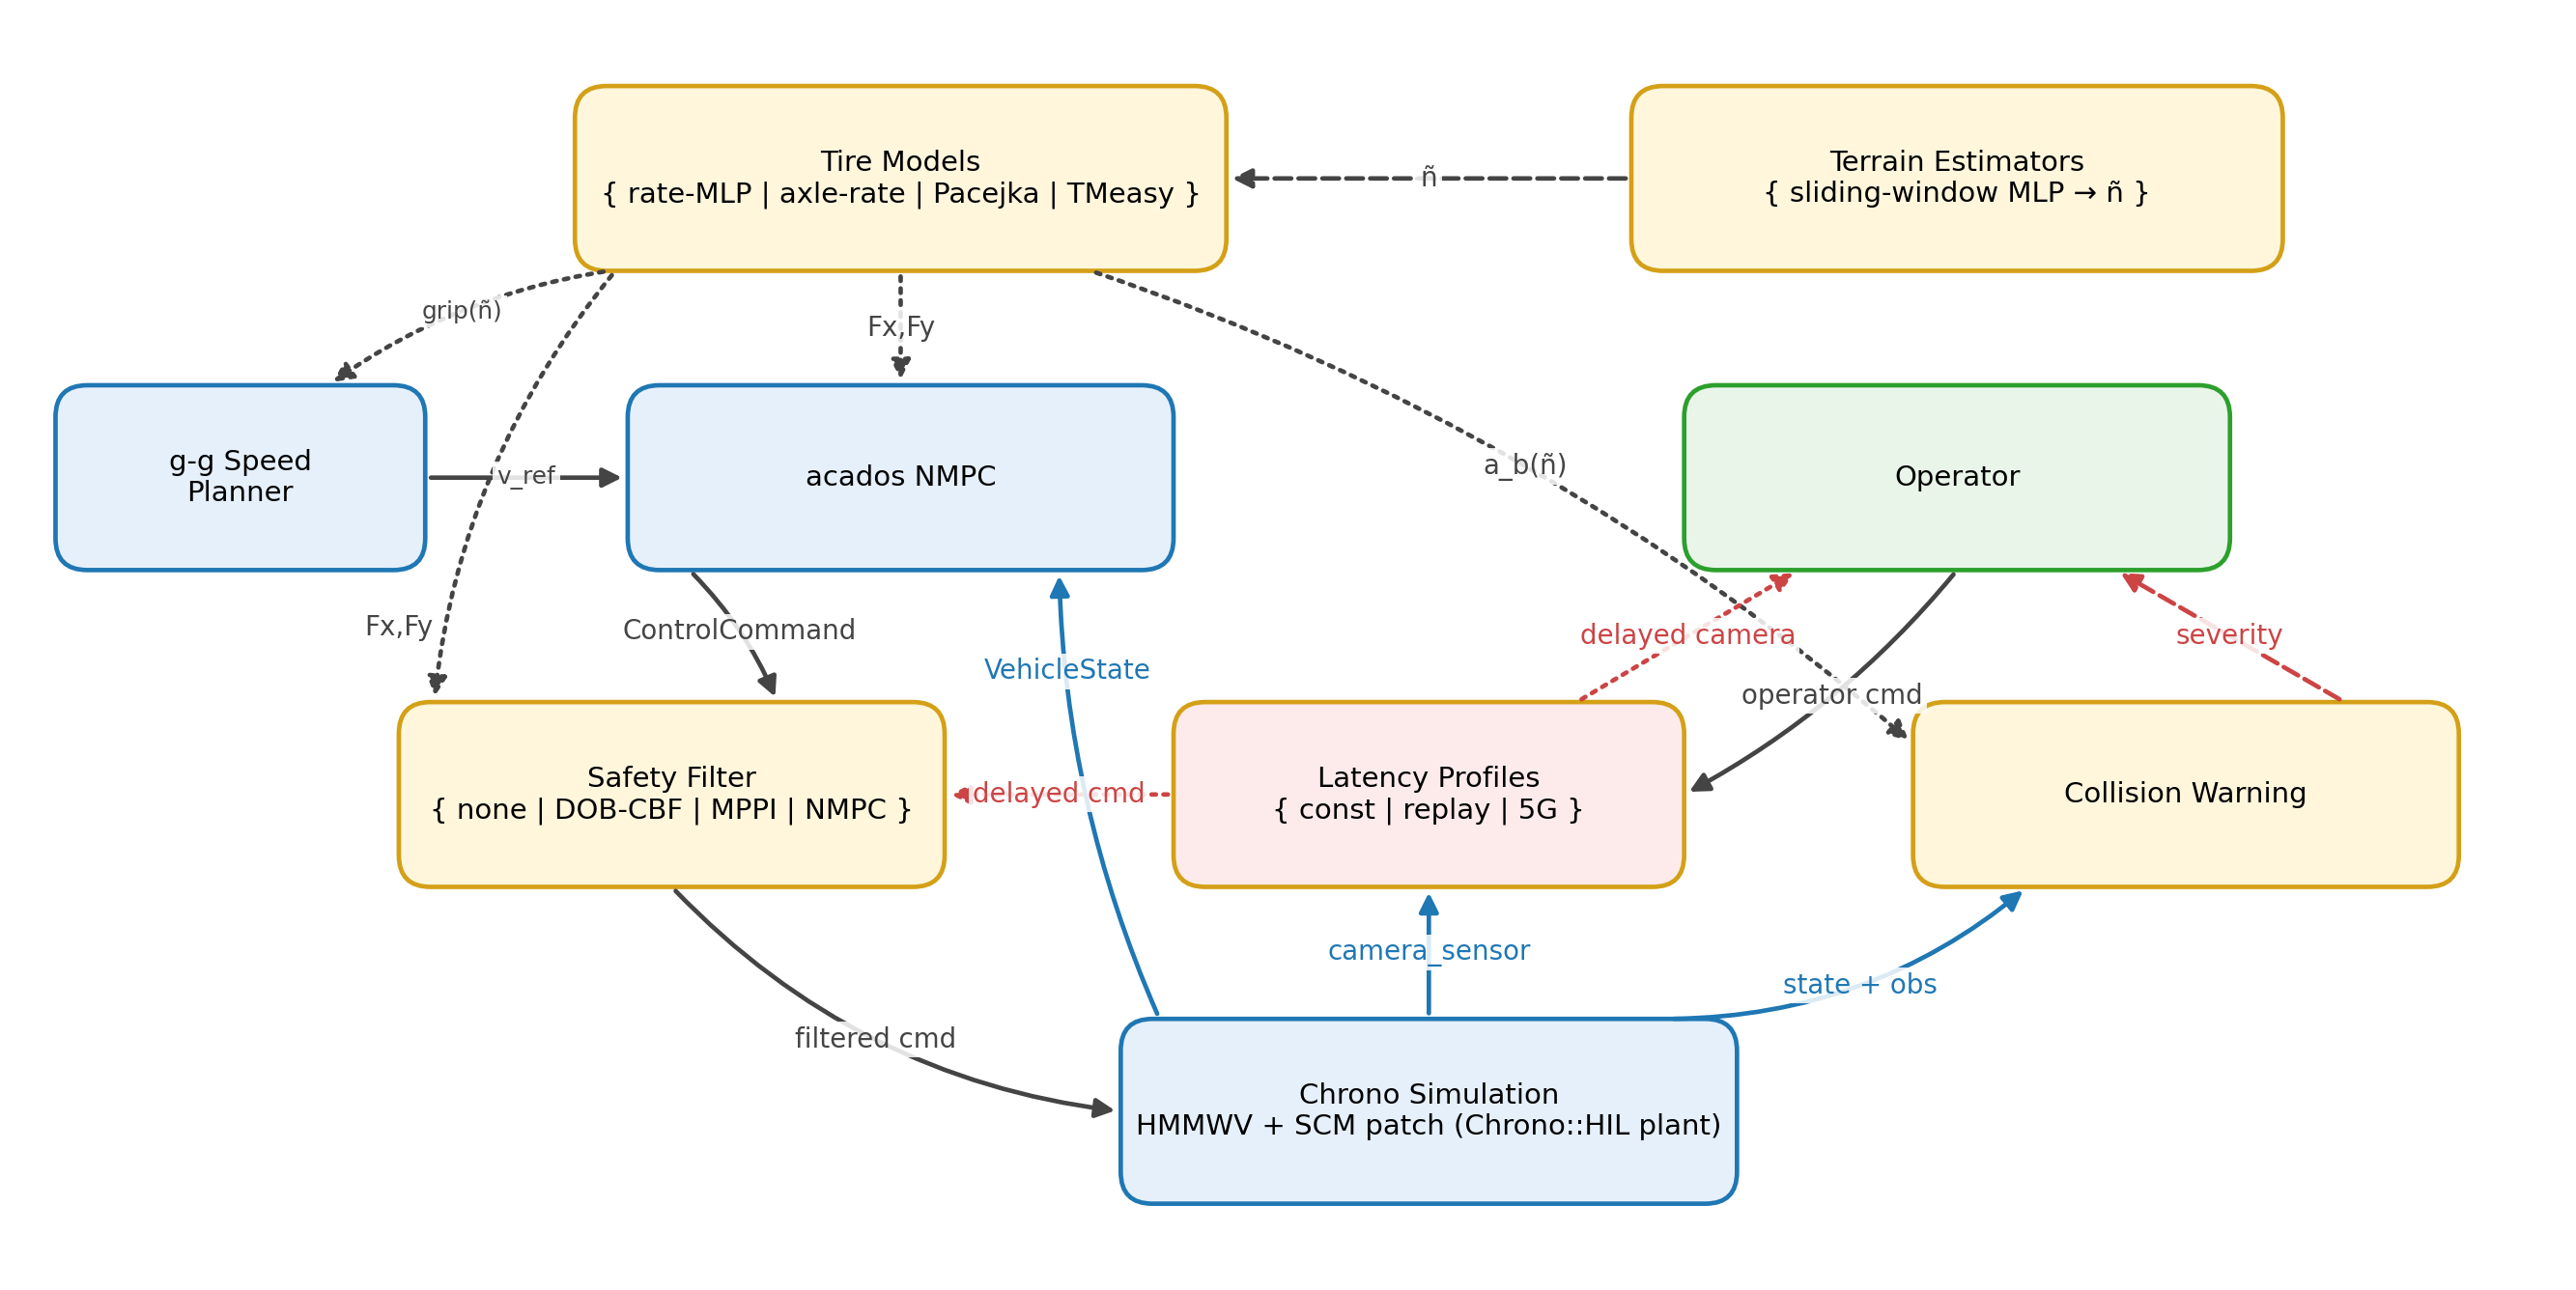
\includegraphics[width=0.92\textwidth]{sys_arch.png}
  \caption{Shared-control framework. Yellow nodes are in-process swap
    points resolved by the corresponding registry; blue/green nodes
    are process-boundary or operator endpoints. Solid arrows are
    runtime data flow over ZeroMQ; dashed arrows are the
    latency-affected operator paths; dotted arrows are tire-surrogate
    queries (build-time CasADi export plus per-tick safety-filter
    rollouts).}
  \label{fig:sysarch}
\end{figure*}

\begin{table}[!t]
  \renewcommand{\arraystretch}{1.15}
  \caption{The six swap points of the framework. Each role is defined
    by one Protocol and resolved through one registry. A conformance
    test instantiates one of each shipped variant and checks it against
    the declared Protocol, so the swap-ability is structural rather
    than rhetorical.}
  \label{tab:swap_points}
  \centering
  \scriptsize
  \setlength{\tabcolsep}{3pt}
  \begin{tabular}{@{}lll@{}}
    \toprule
    \textbf{Role} & \textbf{Protocol method} & \textbf{Shipped variants}\\
    \midrule
    Command source     & \texttt{next\_command}  & NMPC, G29, WASD\\
    Safety filter      & \texttt{filter}         & DOB-CBF, MPPI, NMPC, none\\
    Collision warning  & \texttt{evaluate}       & TTC\\
    Tire model         & \texttt{predict}        & rate-MLP, axle-rate-MLP,\\
                       &                         & Pacejka, TMeasy\\
    Terrain estimator  & \texttt{observe/estimate} & force+proprioceptive UKF,\\
                       &                         & window-MLP, Bekker/NN-UKF\\
    Latency profile    & \texttt{delay}          & constant, replay, learned 5G\\
    \bottomrule
  \end{tabular}
\end{table}

Both processes pace to wall clock, and the benchmark harness
parallelises across runs, so a single workstation completes the
static-terrain tire benchmark of Section~\ref{sec:tires_static} in
well under an hour.

The split between process-boundary contracts (ZMQ messages) and
in-process Protocol contracts is deliberate. Any controller that
subscribes to the vehicle-state message and publishes the
control command can replace the acados NMPC without
modifying the simulator; this is how the tire-model variants of
\S\ref{sec:tires} are evaluated. Human teleoperation is reduced to
the same normalised steering, throttle, and brake command channels
before actuation, so the safety layer screens either autonomous or
human commands behind one contract. Safety filters and the forward
collision warning live behind their own Protocols, are resolved by
name through their registries, and never share state — the warning
attaches to the same vehicle-state stream but never writes to the
command path, so it composes with any selected filter (including the
no-filter case) without re-plumbing. This is what makes the suite a
framework rather than a single monolithic controller demonstration.

%======================================================================
\section{Differentiable SCM Tire Surrogate}
\label{sec:tires}
%======================================================================

A multilayer perceptron (MLP) maps the tire operating point
$(\kappa,\alpha,F_z,u)$, steering rate, and soil parameters
$\boldsymbol{\theta}_{\mathrm{soil}}\!=\!(K_\phi,K_c,n,c,\phi,k)$
(Bekker--Wong-style rig inputs~\cite{Shibly05}) to longitudinal and
lateral tire forces $(F_x, F_y)$. Where Dallas et
al.~\cite{Dallas21} use a static MLP only, we train three variants:
the static baseline, a \emph{rate-augmented} MLP that takes the
steering rate $\dot\delta$ as an explicit input, and an
\emph{axle-rate} MLP with per-axle rate inputs
$(\dot\delta_f,\dot\delta_r)$. All three export as CasADi
expressions through which the acados solver auto-differentiates at
every horizon stage. Two surrogate generations are kept distinct: a
\emph{tire-rig surrogate} trained from controlled single-tire SCM
sweeps (a reproducible baseline against~\cite{Dallas21}) and a
\emph{whole-vehicle surrogate} trained from closed-loop
Chrono::Vehicle HMMWV runs (the model used for the main NMPC and
safety-filter results). The first generation tests whether the
single-tire learning problem is solved; the second tests whether the
controller sees accurate forces in the regimes it actually visits.

\subsection{Training data: from rig sweeps to closed-loop rollouts}
\label{sec:tires_rig_to_cl}
\label{sec:training_data}

The training-data pipeline followed two generations. The first
generation, mirroring the rig protocol of \cite{Dallas21}, drove a
single SCM tire over a Cartesian grid of $(\kappa, \alpha, F_z,
\boldsymbol{\theta}_{\mathrm{soil}})$ and recorded the SCM
ground-truth force at every queried operating point. Rig training is
appealing because every label is exact, no closed-loop feedback
confounds the supervision, and the data collection parallelises
trivially. It produced surrogates with rig-grid coefficient of
determination R$^2 \gtrsim 0.95$ on a held-out rig split, and it is
therefore retained as the controlled baseline. The second generation
targets the controller's deployed operating distribution: rather than
sampling an open-loop tire grid, it collects training tuples from the
closed-loop stack itself so the labels include the high-yaw-rate,
lateral-acceleration, and body-frame force conventions that arise
during aggressive references on deformable soil.

For the closed-loop generation, a parallel pool
of randomised $(\text{terrain}, \text{path}, \text{speed},
\text{bumpiness}, \text{seed})$ scenarios runs the NMPC against
Chrono::Vehicle and logs the live operating point alongside the SCM
ground-truth force. The deployed whole-vehicle surrogate
\texttt{vehicle\_rate\_64\_32\_lhs} is trained on
\textbf{800 such scenarios}, LHS-sampled jointly over the soil
parameters in \texttt{TRAINING\_RANGES\_V6} (Bekker--Mohr box around
clay/dirt/sand) and the maneuver axes — 264 sand, 270 dirt, 266 clay;
214 sinusoidal, 201 right-left, 200 lane-change, 185
double-lane-change; commanded speeds randomised in
$[3,7]\,\mathrm{m/s}$; bumpiness and rock-count randomised; each
scenario simulated for $\sim$10\,s at the controller rate. The
aggregated training table contains approximately $1.85\,\mathrm{M}$ rows of
$(\kappa,\alpha,F_z,u,\dot\delta)\!\to\!(F_x,F_y)$ tuples (front +
rear axle per tick) — fewer samples than the rig's $\sim$100k
single-tire grid but drawn from the operating-point distribution the
deployed MPC actually visits.
The resulting distribution is matched to the
regime the planner actually visits, and the body-frame convention is
enforced at the collection step rather than at the import step. The
three checkpoints used throughout this
paper's pilot sweeps are all closed-loop trained; two rig-trained
checkpoints from the first generation are retained as a baseline so
the rig-versus-closed-loop comparison remains reproducible
(Sec.~\ref{sec:tires_static} selects them as the \texttt{rig\_static}
and \texttt{rig\_rate} model identifiers).

The NMPC queries the surrogate at each stage. The longitudinal
traction budget $F_x^{\mathrm{trac}}$ is evaluated at reference slip
$\kappa_{\mathrm{ref}}$, $\alpha = 0$, with axle loads $F_z$, speed
$u$, and $\boldsymbol{\theta}_{\mathrm{soil}}$ taken from terrain
presets or the online estimator. Cornering forces $F_y$ use the live
operating point $(\kappa, \alpha, F_z, u)$ at each stage.

The two \emph{learned terrain estimators} are trained on deliberately
different data, and the distinction matters for reading their results.
The deployed sliding-window MLP (\texttt{terrain\_window\_mlp},
Sec.~\ref{sec:estimator}) regresses the Bekker exponent $n$ from a
4\,s window of proprioceptive statistics; it is trained on 180 LHS soil
cells $\times$ 20 scenarios, split between closed-loop NMPC tracking
(sinusoidal / lane-change / right-left at $\{4,6,8\}\,\mathrm{m/s}$) and
scripted open-loop cruise-bias runs, at bumpiness $\in\{0,4\}$ only ---
the envelope that bounds its in-distribution claims
(Table~\ref{tab:training_data}). The NN-UKF tire surrogate
(\texttt{vehicle\_fy}, Sec.~\ref{sec:ukf}) is instead trained on 300
\emph{scripted} sinusoidal-steer runs with no controller in the loop,
half at constant open-loop throttle and half under a PI cruise loop,
over a widened soil box so the canonical presets are interior points.
The throttle convention thus differs across models --- the deployed
surrogates see NMPC cruise throttle, the rig surrogate sees none
(fixed rig), and the UKF surrogate sees a mix of constant-open-loop and
PI-cruise throttle --- so each model's accuracy is reported only within
its own excitation envelope.

\begin{table*}[!t]
  \renewcommand{\arraystretch}{1.15}
  \caption{Training-data provenance for the learned models. ``Loop''
    distinguishes scripted open-loop excitation from closed-loop NMPC
    tracking; bumpiness is the terrain-roughness level present during
    training (and hence the envelope within which each model is
    evaluated).}
  \label{tab:training_data}
  \centering
  \small
  \begin{tabularx}{\textwidth}{@{}L L L c L@{}}
    \toprule
    \textbf{Model (role)} & \textbf{Loop / excitation} & \textbf{Throttle} & \textbf{Bumpiness} & \textbf{Soil / $n$ coverage}\\
    \midrule
    \texttt{rig\_rate} (rig tire baseline) & open-loop single-tire rig, scripted $\kappa/\alpha$ & --- (fixed rig) & --- & LHS around clay/dirt/sand\\
    \texttt{vehicle\_rate} (deployed NMPC tire) & closed-loop NMPC, 4 paths & NMPC cruise, $[3,7]\,\mathrm{m/s}$ & $\{0,2,4\}$ & full Bekker--Mohr LHS box\\
    \texttt{terrain\_window\_mlp} (deployed estimator) & closed-loop NMPC $+$ scripted open-loop & NMPC $+$ cruise-bias & $\{0,4\}$ & $n\in[0.40,1.30]$, 180 LHS cells\\
    \texttt{vehicle\_fy} (NN-UKF tire, Sec.~\ref{sec:ukf}) & scripted sinusoidal steer, no controller & half const.\ OL / half PI-cruise & $0$ & widened $n\in[0.35,1.35]$\\
    \bottomrule
  \end{tabularx}
\end{table*}

\subsection{Static-terrain benchmark}
\label{sec:tires_static}

The standard MPC is swept over the three deployable tire models
(Pacejka, TMeasy, and the deployed vehicle NN rate-MLP) across all
three terrains (clay, dirt, sand), three reference paths (sinusoidal,
lane-change, right-left), three reference speeds
$v_{\mathrm{ref}}\in\{5,7,9\}\,\mathrm{m/s}$, three bumpiness levels,
and five random seeds, for a total of 1215 closed-loop trials. Sensor
noise is enabled in every trial. To keep the comparison fair, the
analytical baselines are \emph{not} run at rigid-road defaults: their
peak lateral friction is calibrated to a single global $\mu=0.42$ by
least-squares fit to the pooled SCM tire-rig forces across the soil box
(the SCM peak $|F_y|/F_z$ ranges from $\approx 0.18$ clay-like to
$\approx 0.47$ sand-like, far below a rigid road), with the
magic-formula and TMeasy shape factors kept at their standard values;
one global set is used for every terrain because the controller has no
per-terrain knowledge. This removes the rigid-road over-grip that
otherwise inflates the baseline error, so the reported gap reflects what
a fixed analytical parameterisation structurally cannot capture, not a
tuning deficit.
Table~\ref{tab:tires_static} reports the mean and standard deviation
of root-mean-square crosstrack error (RMS CTE), speed retention
ratio, and solver wall time across the matrix. The neural row is the
deployed whole-vehicle surrogate; the rig-trained checkpoints are
retained in the benchmark suite as explicit \texttt{rig\_static} and
\texttt{rig\_rate} baselines for reproducing the rig-to-vehicle
comparison. Fig.~\ref{fig:tires_static_heatmap} breaks the same matrix
out per (terrain, path), which makes the analytical-baseline failure
mode at dirt/sinusoidal and dirt/right-left visible at a glance.

\begin{table}[!t]
  \renewcommand{\arraystretch}{1.15}
  \caption{Tire-model benchmark over the full 1215-run matrix (405 runs
    per model), against \emph{SCM-calibrated} analytical baselines
    (single global $\mu\!=\!0.42$, Sec.~\ref{sec:tires_static}). The
    deployed vehicle NN rate-MLP attains the lowest mean RMS CTE,
    $46$--$48\,\%$ below the analytical baselines; the per-model
    \emph{medians} are close ($0.12$--$0.15\,\mathrm{m}$), so the NN's
    gain is in the tail --- the Pacejka and TMeasy rows carry large
    right-skewed standard deviations ($0.44$--$0.45$ vs.\ $0.17$) from
    off-nominal dirt scenarios (Fig.~\ref{fig:tires_static_heatmap})
    that the NN suppresses. All models retain similar speed because
    this controlled comparison fixes the speed reference to the
    geometric curvature profile across every tire model (the deployed
    terrain-aware speed planner of Sec.~\ref{sec:speedplan} is held out
    so the comparison isolates the tracking tire model), so the
    reference, not the tire force model, binds speed here. The NN's higher solve time
    reflects the embedded surrogate evaluation.}
  \label{tab:tires_static}
  \centering
  \begin{tabular}{lccc}
    \toprule
    \textbf{Tire model} & \textbf{RMS CTE (m)} & \textbf{Speed} & \textbf{Solve}\\
                         &                       & \textbf{ratio} & \textbf{(ms)}\\
    \midrule
    Pacejka                       & $0.35 \pm 0.45$ & $0.66$ & $4.2$\\
    TMeasy                        & $0.34 \pm 0.44$ & $0.65$ & $4.6$\\
    \textbf{Vehicle NN rate-MLP}  & $\mathbf{0.18 \pm 0.17}$ & $0.67$ & $14.0$\\
    \bottomrule
  \end{tabular}
\end{table}

\begin{figure}[!t]
  \centering
  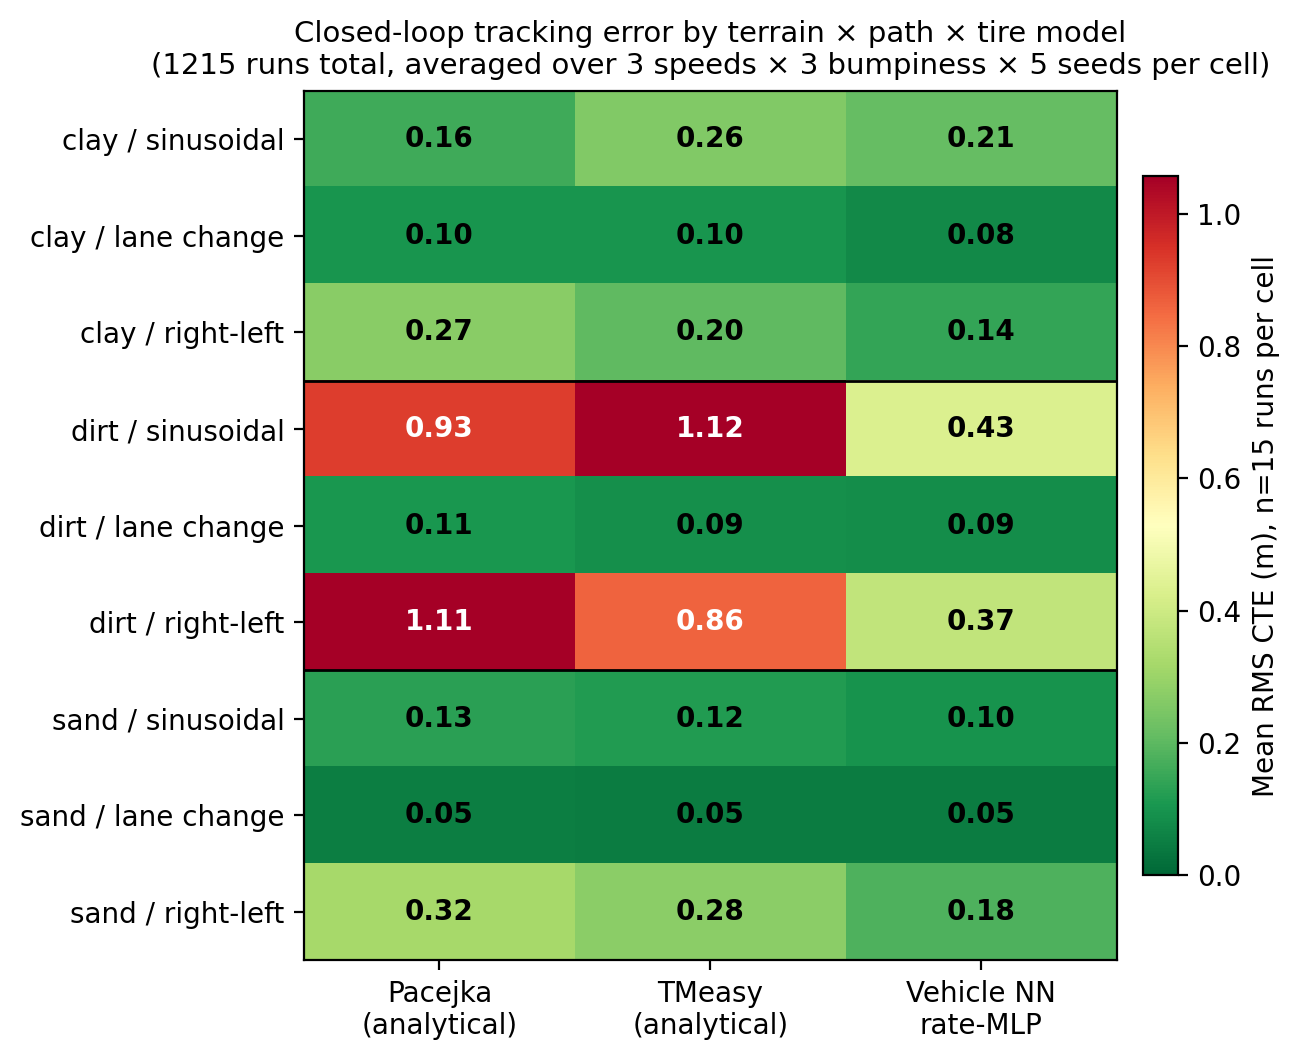
\includegraphics[width=\columnwidth]{cte_master_heatmap.png}
  \caption{Closed-loop RMS CTE per (terrain, path) cell across the
    broader 1215-run sweep (3~speeds $\times$ 3~bumpiness $\times$
    5~seeds per cell). The analytical baselines (Pacejka, TMeasy)
    track well on clay and sand but diverge on dirt/sinusoidal
    ($\sim\!1.0\,\mathrm{m}$) and dirt/right-left
    ($0.9$--$1.2\,\mathrm{m}$), where the curvature-limited reference
    combines with off-nominal sinkage to produce a regime the analytical
    force laws do not cover even after SCM calibration. The Vehicle NN
    rate-MLP suppresses those tails to $0.4$--$0.6\,\mathrm{m}$ while
    matching the calibrated baselines on the benign cells. This per-scenario
    view is what motivates the live-estimator benchmark in
    Sec.~\ref{sec:tires_estimator}.}
  \label{fig:tires_static_heatmap}
\end{figure}

\subsection{Live-estimator-conditioned benchmark}
\label{sec:tires_estimator}

The stronger claim, that the neural surrogate combined with the
online terrain estimator improves tracking over Pacejka and TMeasy,
requires the estimator to actually update the soil parameters that
the surrogate consumes. The same model set is therefore re-evaluated
with the online estimator enabled, using a 20-second simulation
window with key performance indicators (KPIs) computed after an
8-second post-convergence cutoff.
Table~\ref{tab:tires_estimator} reports the result;
Fig.~\ref{fig:tires_estimator_heatmap} shows the per-scenario
heatmap. Because this regime conditions on the live estimator (not the
static terrain prior of Table~\ref{tab:tires_static}) and reports
\emph{medians} over the larger 1620-run matrix, its analytical-baseline
numbers are not directly comparable to Table~\ref{tab:tires_static}'s
mean$\pm$std over the 1215-run static matrix; the two report the
static-prior and live-estimator regimes respectively.

Two points are needed to read Table~\ref{tab:tires_estimator}
honestly. First, the \texttt{static} neural row is conditioned on the
matched terrain preset and therefore behaves as a near-oracle
reference, whereas the \texttt{+estimator} row must recover the soil
parameters online from inertial and wheel-speed signals alone. The
estimator variant nearly matches that near-oracle row
(median $0.177$ vs.\ $0.174\,\mathrm{m}$, a $3\,\mathrm{mm}$ gap whose
$95\,\%$ bootstrap confidence intervals, $[0.150,0.191]$ and
$[0.142,0.191]\,\mathrm{m}$, overlap --- statistically indistinguishable)
while requiring no prior terrain knowledge, and both NN rows reduce
median RMS CTE by $37$--$38\,\%$ relative to the SCM-calibrated Pacejka
and TMeasy baselines. The deployable claim is therefore that the
estimator recovers most of the oracle-prior benefit without that prior,
not that it improves on a correct prior. Second, the per-row distributions are
strongly right-skewed by a few high-error scenarios (mostly
Pacejka and TMeasy on dirt at $v_{\mathrm{ref}}\!=\!7\,\mathrm{m/s}$,
where the analytical baselines collide with the curvature limit);
Fig.~\ref{fig:tires_estimator_heatmap} shows the full distribution per
variant so the median and tail behaviour are both visible.

\begin{table}[!t]
  \renewcommand{\arraystretch}{1.15}
  \caption{Live-estimator-conditioned tire-model benchmark, full
    1620-run matrix (405 per variant), KPI window from $t=8\,\mathrm{s}$.
    Values are \emph{median} RMS CTE: the per-variant distributions are
    strongly right-skewed by a few high-error dirt scenarios
    (Fig.~\ref{fig:tires_estimator_heatmap}), so the median is the
    representative statistic. The \texttt{static} neural row is
    conditioned on the matched terrain preset (near-oracle); the
    \texttt{+estimator} row runs the deployed force+proprioceptive
    Fused-UKF (Sec.~\ref{sec:ukf}) online and nearly matches the oracle
    (median $0.177$ vs.\ $0.174\,\mathrm{m}$, a $3\,\mathrm{mm}$ gap with
    overlapping $95\,\%$ bootstrap CIs). Both NN rows reduce median RMS
    CTE by $37$--$38\,\%$ relative to the \emph{SCM-calibrated}
    analytical baselines (single global $\mu\!=\!0.42$).}
  \label{tab:tires_estimator}
  \centering
  \setlength{\tabcolsep}{4pt}
  \begin{tabular}{lccc}
    \toprule
    \textbf{Variant} & \textbf{CTE (m)} & \textbf{vs.\ Pacejka} & \textbf{vs.\ TMeasy}\\
    \midrule
    Pacejka (static)            & $0.28$ & ---       & ---\\
    TMeasy (static)             & $0.28$ & ---       & ---\\
    NN rate-MLP (static)        & $0.17$ & $-38\,\%$ & $-38\,\%$\\
    \textbf{NN rate-MLP $+$ estimator} & $\mathbf{0.18}$ & $\mathbf{-37\,\%}$ & $\mathbf{-37\,\%}$\\
    \bottomrule
  \end{tabular}
\end{table}

A separate ablation isolates the deployable value of the estimator
explicitly. Holding the controller's static terrain prior at dirt
regardless of the plant terrain gives the
wrong-prior baseline, comparable directly against the matched-prior
oracle and the estimator-on variant on the same matrix
(clay$+$sand $\times$ sinusoidal $\times$ $v\in\{5,7\}\,\mathrm{m/s}$
$\times$ $2$ seeds, $8$ runs per variant).
Table~\ref{tab:wrong_prior} reports the result. On clay the wrong
dirt prior gives RMS CTE $1.54\,\mathrm{m}$, the estimator-on variant
(the deployed Fused-UKF, Sec.~\ref{sec:ukf}) adapts from the same dirt
initialisation and recovers to $0.72\,\mathrm{m}$, on par with the
matched-prior oracle ($0.75\,\mathrm{m}$) -- the estimator closes
essentially the entire prior-mismatch gap on the harder terrain.

\begin{table}[!t]
  \renewcommand{\arraystretch}{1.10}
  \caption{Wrong-prior ablation: RMS CTE (m) when the controller's
    static terrain prior is fixed to dirt regardless of plant terrain,
    compared against the matched-prior near-oracle and the estimator-on
    variant. $24$ runs total ($8$ per variant). The matrix excludes
    dirt (where the dirt-prior is by construction matched) and the
    other paths/bumpiness levels of Table~\ref{tab:tires_estimator};
    absolute numbers are therefore not comparable across the two
    tables. The estimator nearly recovers the matched-prior
    performance from a wrong initialisation on clay; matched and
    wrong priors both yield low error on sand because dirt is closer to sand
    than to clay on the soil-parameter manifold.}
  \label{tab:wrong_prior}
  \centering
  \begin{tabular}{lccc}
    \toprule
    \textbf{Variant} & \textbf{Clay} & \textbf{Sand} & \textbf{Mean}\\
    \midrule
    Matched static prior (oracle) & $0.751$ & $0.059$ & $0.405$\\
    Wrong (dirt) static prior     & $1.538$ & $0.064$ & $0.801$\\
    \textbf{Estimator-on (dirt $\to$ adapt)} & $\mathbf{0.723}$ & $\mathbf{0.058}$ & $\mathbf{0.391}$\\
    \bottomrule
  \end{tabular}
\end{table}

\begin{figure}[!t]
  \centering
  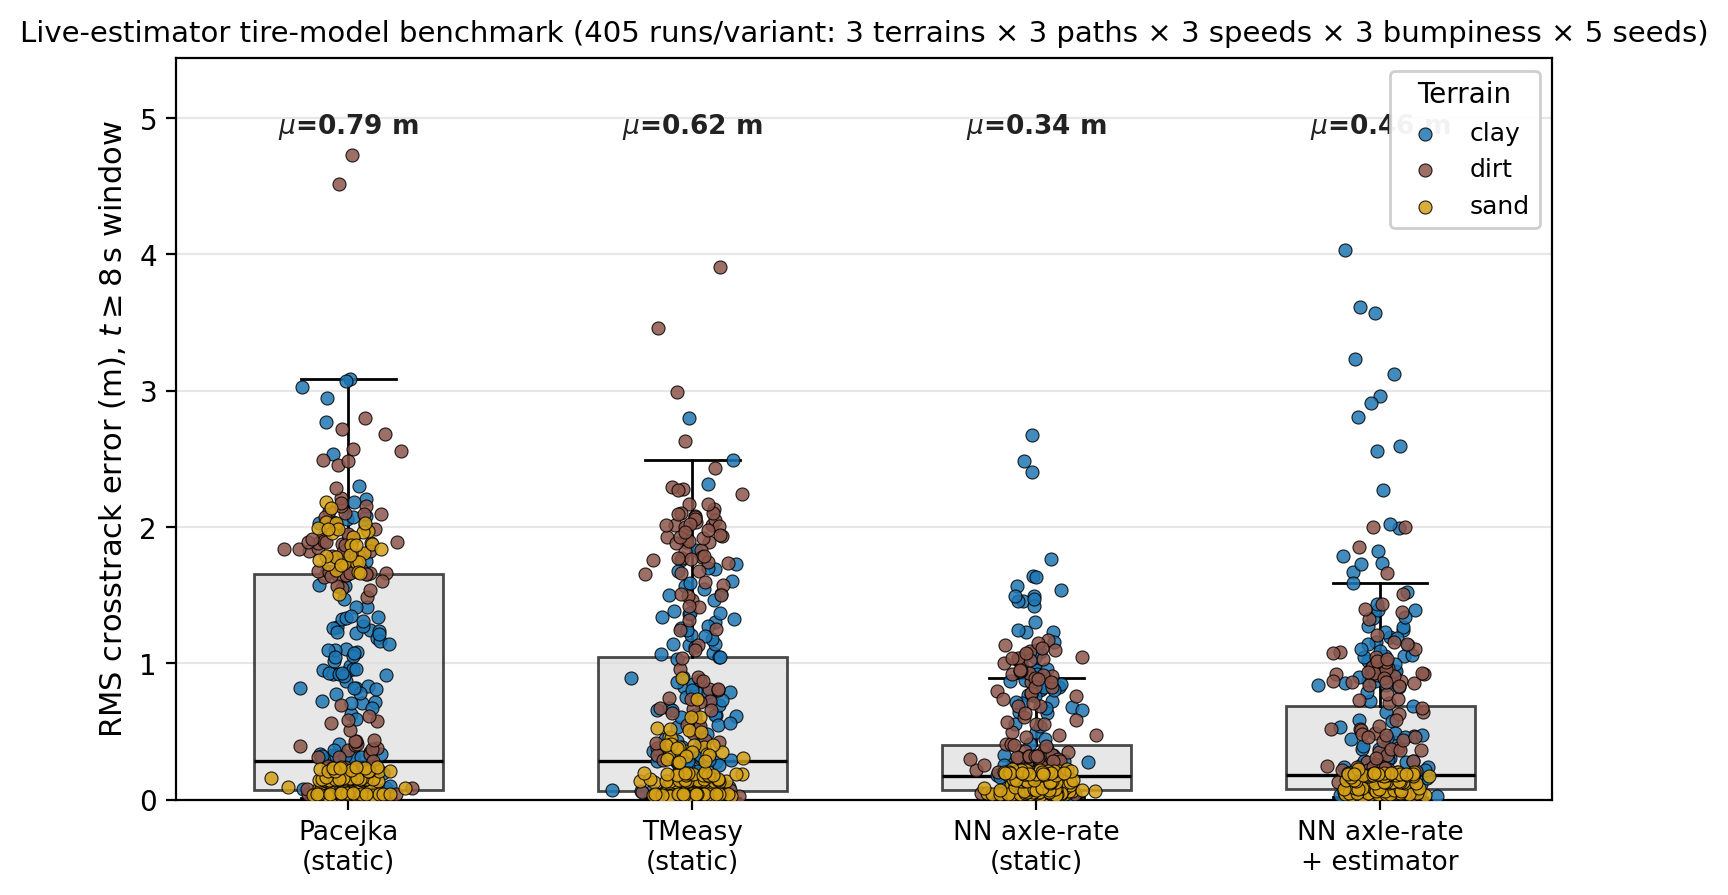
\includegraphics[width=\columnwidth]{tire_model_with_estimator_rms_cte_heatmap.png}
  \caption{Same benchmark, RMS CTE distribution per variant.
    Box plots show interquartile range and median across all 405 runs
    per variant; jittered scatter points are coloured by terrain
    (clay, dirt, sand). The two analytical baselines (Pacejka, TMeasy)
    carry long right tails driven by a few dirt cases at higher
    $v_{\mathrm{ref}}$; both neural variants compress the distribution
    sharply. The estimator-on variant nearly matches the matched-prior
    static row, the deployable claim of Sec.~\ref{sec:tires_estimator}.}
  \label{fig:tires_estimator_heatmap}
\end{figure}

\subsection{Controlled rig-versus-whole-vehicle comparison}
\label{sec:tires_rig_vs_vehicle}

The rig-vs-whole-vehicle question motivating
Sec.~\ref{sec:tires_rig_to_cl} is settled by a controlled retrain
that removes two confounds present in the earlier comparison: rig
checkpoints used smaller MLPs (16-4, 16-8) than vehicle checkpoints
(32-16), and the vehicle training set jittered scenarios around the
three canonical deployment terrains rather than sampling broadly. We
retrain:

\begin{itemize}
\item three rig checkpoints (32-16 static, 32-16 rate, 64-32 rate) on
  the existing 100k single-tire SCM CSVs;
\item three whole-vehicle checkpoints (matched architectures) on a
  fresh 800-scenario closed-loop dataset that LHS-samples
  $\boldsymbol\theta_{\mathrm{soil}}$ across the same Bekker--Mohr box
  the rig uses (\texttt{TRAINING\_RANGES\_V6}; no canonical-preset
  jitter).
\end{itemize}

Offline force prediction on a held-out LHS test slice exposes the
generalisation gap that the canonical-jitter eval set previously
hid: the legacy whole-vehicle checkpoints' $R^2(F_y)$ drops from
$+0.58$ on canonical-jitter data to $-0.30$ on LHS-terrain data,
while the LHS-trained replacements hold $R^2 \approx 0.71$ on both
eval sets. The retrained vehicle MLPs were not better at predicting
in-distribution data; the legacy MLPs had been over-fitting the
deployment-terrain neighbourhood.

The controlled closed-loop tire-model sweep (432 runs, 6 surrogates
$\times$ 3 terrains $\times$ 3 paths $\times$ 2 speeds $\times$ 2
bumpiness $\times$ 2 seeds; planner-only, sensor noise on) is
summarised in Table~\ref{tab:tires_rig_vs_vehicle}. The pre-retrain
rig-trained advantage narrows substantially:

\begin{itemize}
\item Static MLPs: the rig surrogate remains decisively better
  ($0.085\,\mathrm{m}$ vs $0.112\,\mathrm{m}$, 24\,\%).
\item Rate MLPs (32-16): rig and vehicle match at $0.090\,\mathrm{m}$.
\item Rate MLPs (64-32): tied within noise
  ($0.097$ vs $0.099\,\mathrm{m}$).
\end{itemize}

Per-tick force-prediction smoothness explains the shrinking gap:
aggregated over the 432 runs, the LHS-trained vehicle surrogates have
$\mathrm{std}(\dot F_y^{\mathrm{pred}})$ around $16$-$20$~kN/s, much
closer to the rig surrogates' $14$~kN/s (the $32$-$16$ rig\_rate
variant) than the legacy vehicle MLPs' $40$~kN/s. Wider
training-terrain coverage acts as an effective low-pass on the
closed-loop SCM signal in the same way LHS-independent sampling did
for the rig.

\begin{table}[!t]
  \renewcommand{\arraystretch}{1.15}
  \caption{Controlled rig-vs-whole-vehicle sweep (432 closed-loop
    runs, planner-only, sensor noise on). Matched architecture in
    each pair; rig retrains use the kept 100k LHS rig CSV, vehicle
    retrains use a fresh 800-scenario LHS-terrain closed-loop dataset.
    The earlier small-capacity rig and vehicle checkpoints are
    preserved in the benchmark suite for reproducibility.}
  \label{tab:tires_rig_vs_vehicle}
  \centering
  \footnotesize
  \begin{tabular}{lccc}
    \toprule
    \textbf{Surrogate (32-16 / 64-32 paired)} & \textbf{RMS CTE} & \textbf{Speed} & \textbf{Solve}\\
                                              & \textbf{(m)} & \textbf{ratio} & \textbf{(ms)}\\
    \midrule
    Rig static (32-16)        & $\mathbf{0.085}$ & $0.73$ & $8.0$\\
    Vehicle static (32-16)    & $0.112$          & $0.73$ & $8.1$\\
    Rig rate (32-16)          & $0.090$          & $0.73$ & $10.1$\\
    Vehicle rate (32-16)      & $0.090$          & $0.72$ & $10.3$\\
    Rig rate (64-32)          & $0.097$          & $0.73$ & $12.6$\\
    Vehicle rate (64-32)      & $0.099$          & $0.72$ & $13.0$\\
    \bottomrule
  \end{tabular}
\end{table}

\begin{figure}[!t]
  \centering
  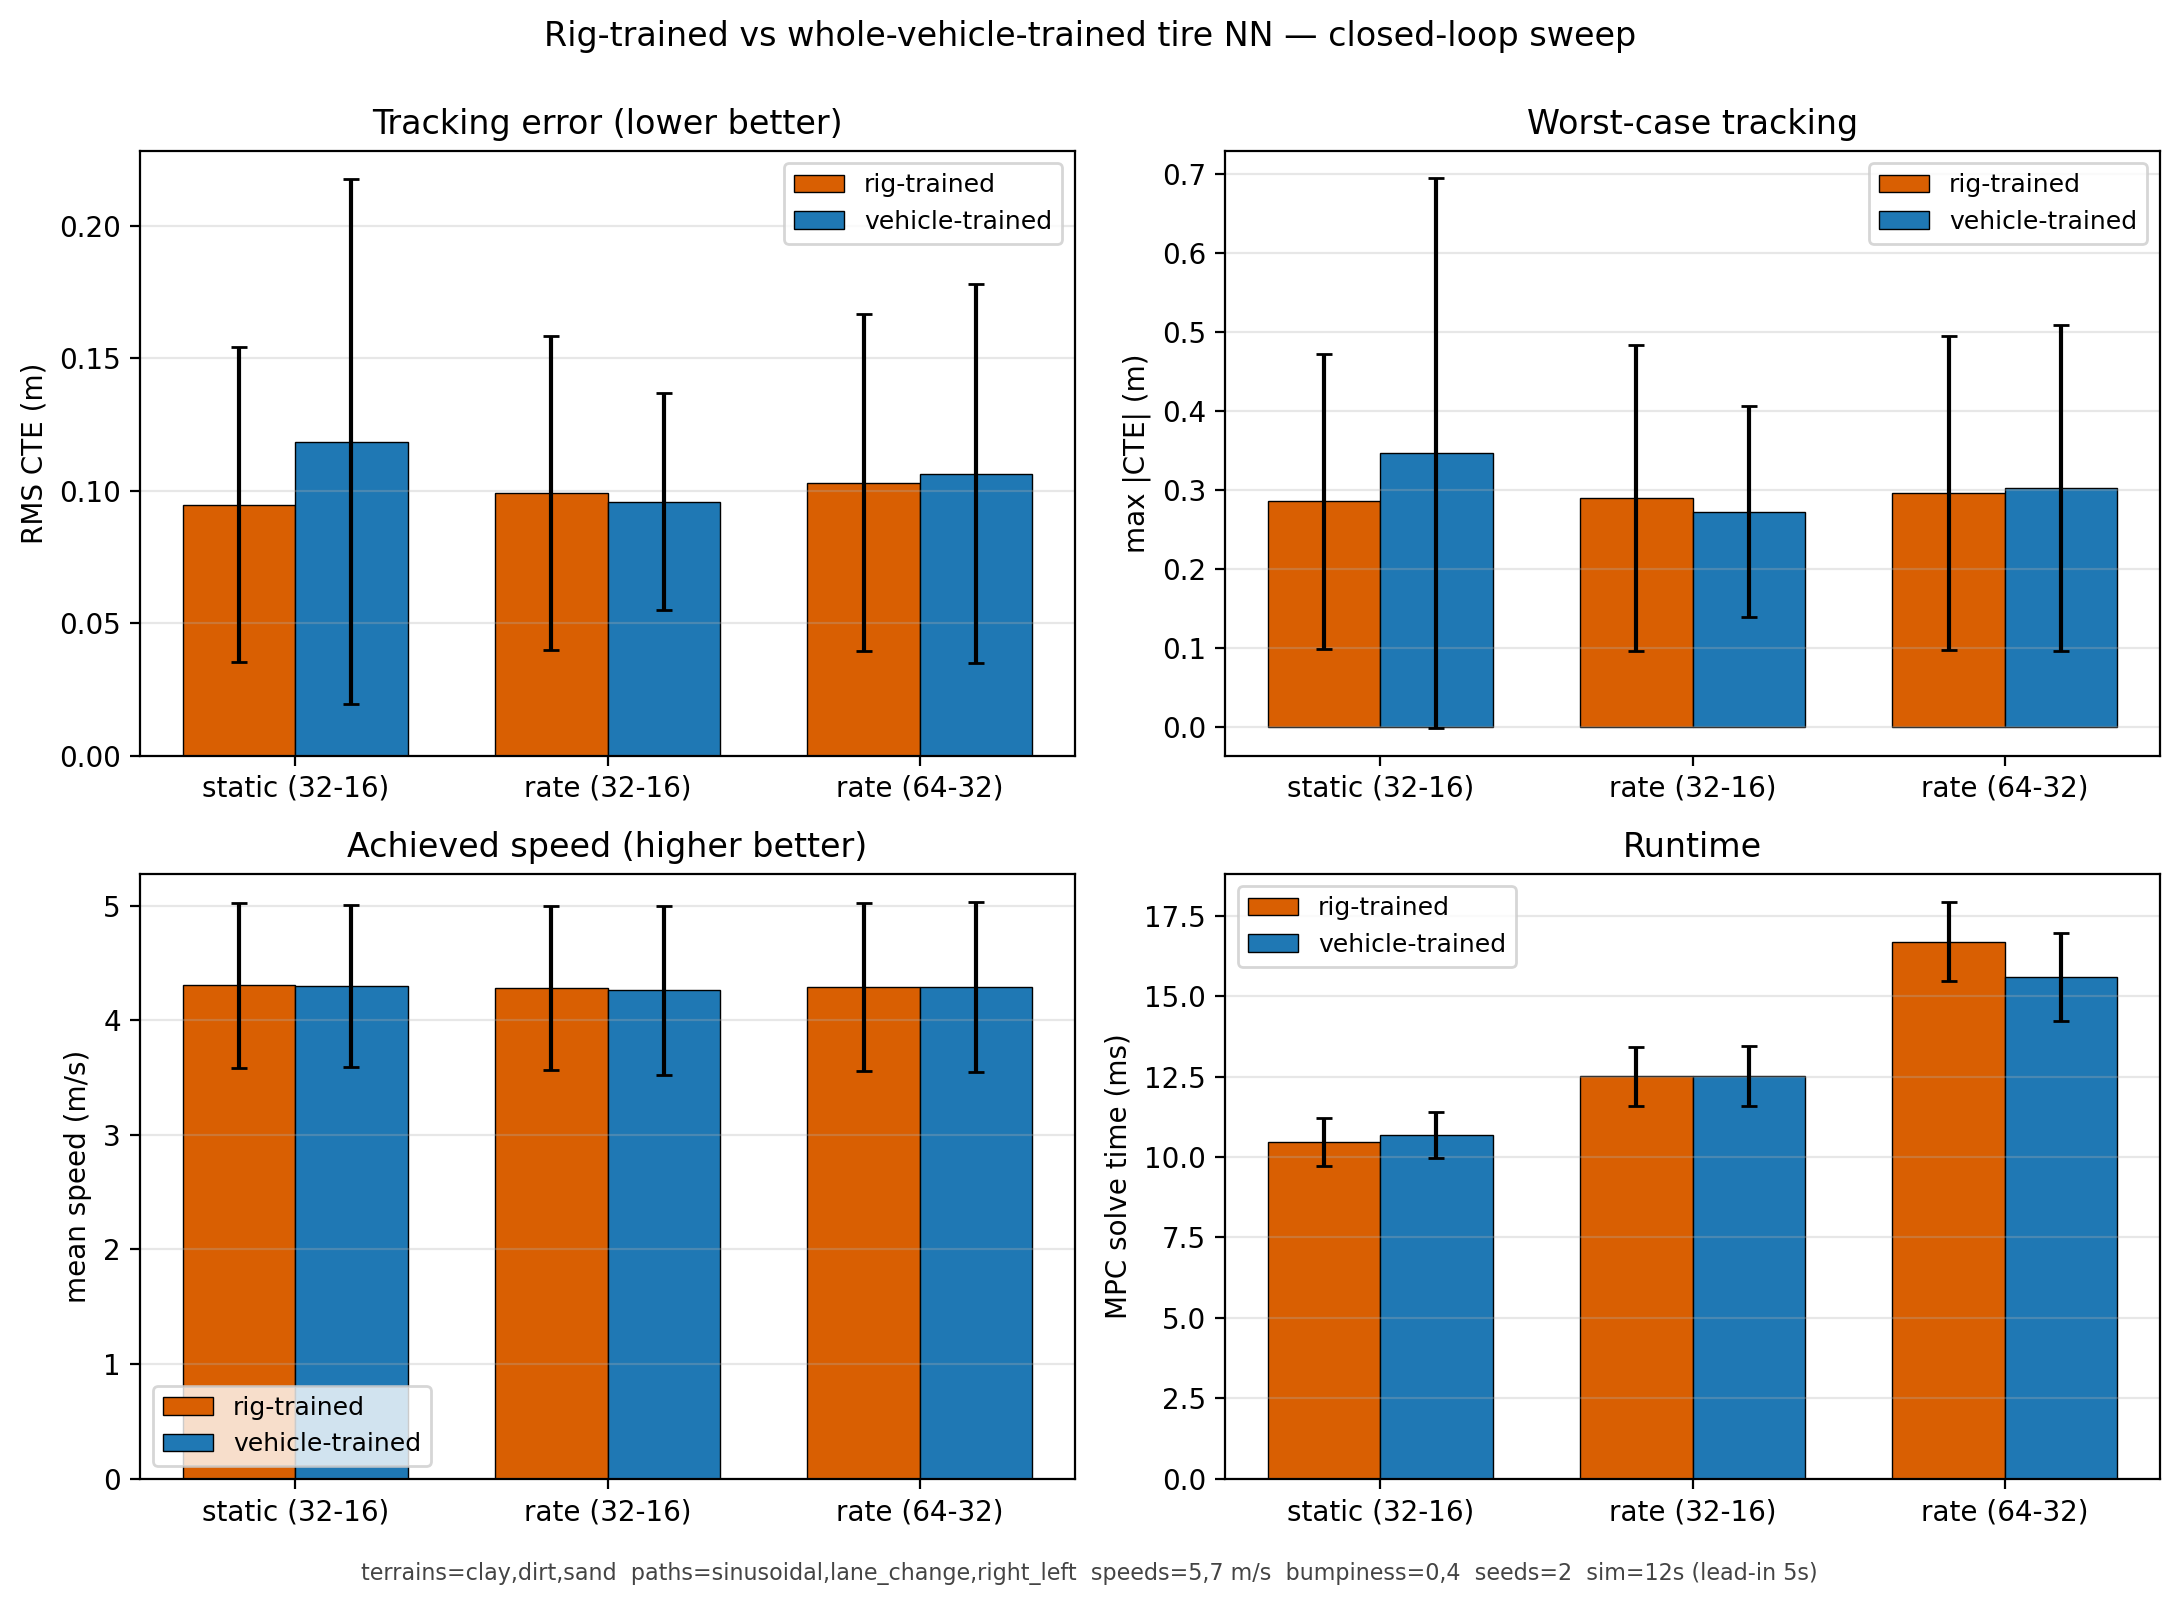
\includegraphics[width=\columnwidth]{rig_vs_vehicle_paired_bars_v2.png}
  \caption{Aggregate metrics over the 432-run controlled sweep, six
    surrogates paired by architecture and signature. RMS CTE,
    worst-case $|\mathrm{CTE}|$, achieved speed, and solver wall time
    on the same matrix. Bars are mean $\pm$ s.d.~across 72 cells per
    surrogate. The pre-retrain rig-trained advantage narrows
    to a static-only effect once architecture is matched and the
    whole-vehicle training data is LHS-sampled over the same Bekker--
    Mohr box the rig uses.}
  \label{fig:rig_vs_vehicle_paired}
\end{figure}

\paragraph{Force-RMSE vs control-RMS-CTE picture is not the same metric.}
The CTE numbers in Table~\ref{tab:tires_rig_vs_vehicle} are within
1\,cm of each other across the four mid-size variants. To unpack what
each surrogate is actually doing during those runs, we replay all
four surrogates on twelve logged trajectories (one of which is shown
in Fig.~\ref{fig:rig_vs_vehicle_4way}), computing per-tick front-axle
$|\Delta F_y|$ against the Chrono ground truth without re-running the
simulator. Mean RMSE across the twelve scenarios:

\begin{center}\footnotesize
\setlength{\tabcolsep}{4pt}
\begin{tabular}{@{}lc@{}}
\textbf{Surrogate}                            & \textbf{Mean RMSE $F_y$ (N)} \\ \midrule
Rig static (32-16)                            & $632$ \\
Vehicle static (32-16)                        & $645$ \\
Rig rate (64-32)                              & $671$ \\
Vehicle rate (64-32, deployed)                & $706$ \\
Ensemble (0.4 rig + 0.6 vehicle, rate)        & $637$ \\
\end{tabular}
\end{center}

The deployed vehicle rate surrogate is the
\emph{worst} of the four on this force-RMSE metric, yet it is also
the most reliable on closed-loop tracking. A six-scenario CTE
comparison driving the standard MPC with each surrogate
shows the static and rate vehicle surrogates within 5\,cm of each
other on five of six scenarios --- and a single catastrophic failure
on clay/right-left at $v_{\mathrm{ref}}=7\,\mathrm{m/s}$ where
the static surrogate degrades to $1.07\,\mathrm{m}$ RMS CTE while
the rate surrogate stays at $0.16\,\mathrm{m}$. The mean RMS CTE
across the six scenarios is therefore $0.18\,\mathrm{m}$ for the
rate variant and $0.33\,\mathrm{m}$ for the static variant; excluding
the catastrophic case they match at $0.185\,\mathrm{m}$.  The
rate-augmented variants trade their force-RMSE deficit for a
lower-bandwidth, lower-amplitude $F_y$ trace whose under-prediction at
transient peaks (the controller that collected the LHS data planned
conservatively, so the training distribution underweights
extreme-slip excursions) is compensated by a smoother MPC control
output and an absence of the catastrophic failure mode the static
checkpoint exhibits. A simple $w=0.4$ rig-plus-vehicle ensemble
cancels the opposing biases at zero deployment cost (RMSE drops to
637\,N, a 5\,\% improvement over vehicle alone), and is the
recommended default for downstream force-prediction consumers such
as the MPPI filter.

\begin{figure}[!t]
  \centering
  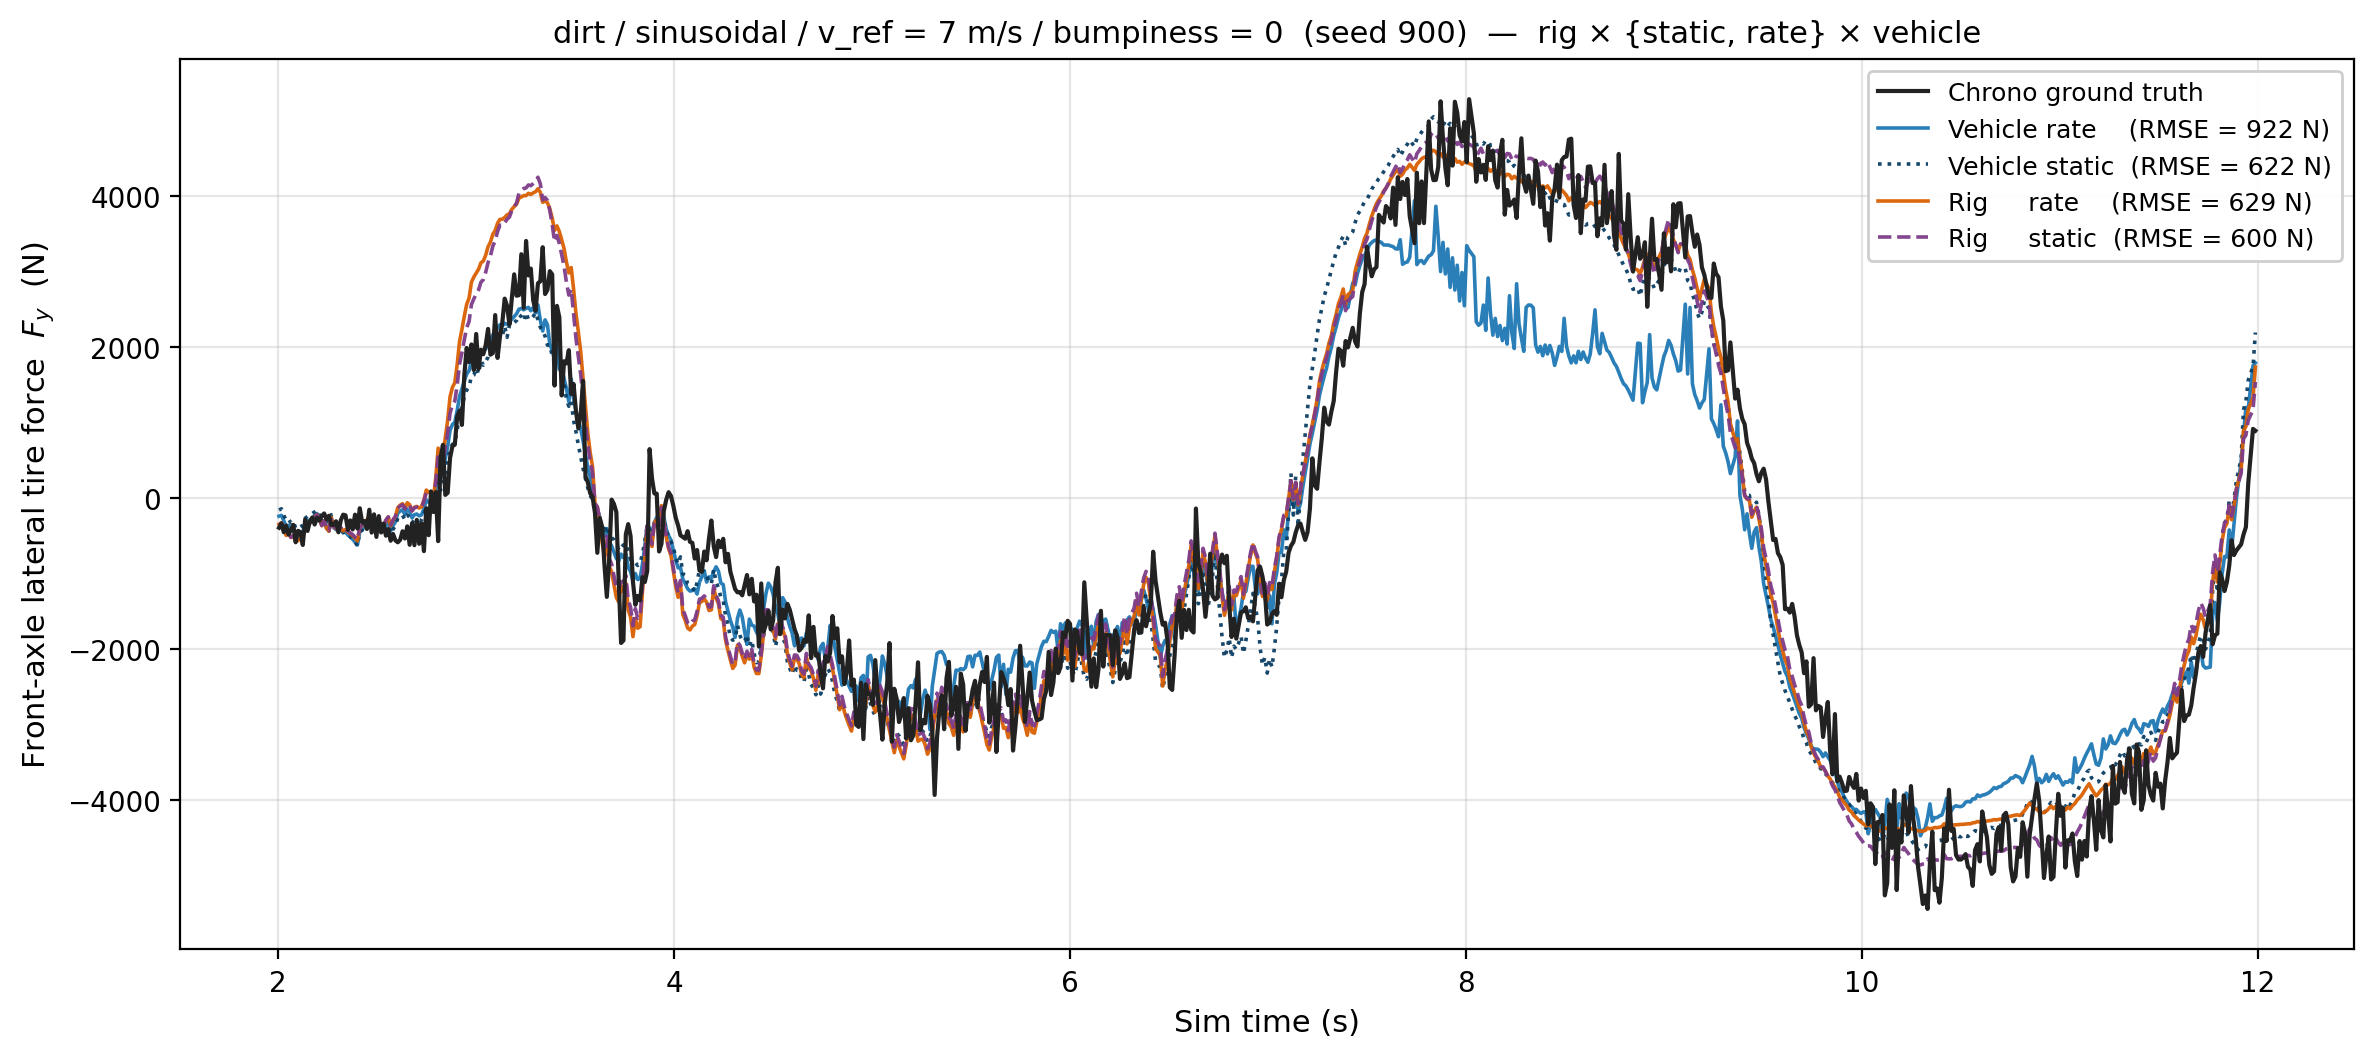
\includegraphics[width=\columnwidth]{fig1_force_4way_dirt_sinusoidal_v7_b0_s900.png}
  \caption{One representative scenario from the four-way comparison
    (dirt, sinusoidal, $v_{\mathrm{ref}}=7\,\mathrm{m/s}$, $b=0$),
    front-axle $F_y$. Black is Chrono ground truth; the four
    coloured traces are the deployed vehicle rate surrogate (light
    blue), the vehicle static surrogate (dark blue dotted),
    rig rate (orange), and rig static (purple dashed). Vehicle rate
    consistently under-predicts the peaks; the rig variants
    over-predict the same peaks; both static checkpoints track the
    envelope most tightly. The deployed default still attains the lowest RMS
    CTE but at the cost of the largest force-RMSE.}
  \label{fig:rig_vs_vehicle_4way}
\end{figure}

In an extended sweep that pairs each surrogate with one of four
safety filters (none / DOB-CBF / MPPI / NMPC) and 5 randomly placed
obstacles, the right surrogate depends on the consuming filter
(Table~\ref{tab:rig_vs_vehicle_filter}). DOB-CBF reads the surrogate
as a static traction-ceiling query and pairs cleanly with the rig
MLP (zero collisions across 16 runs in this matrix); MPPI rolls the
surrogate forward many times per tick and similarly prefers the
smoother rig surface; NMPC's short-horizon SLSQP and the planner-only
no-filter case prefer the LHS-vehicle MLP's better in-distribution
magnitude accuracy. An earlier, uncontrolled comparison showed the
same qualitative flip but with much larger margins, driven by
capacity and noise asymmetries between the models; the controlled
sweep below removes those confounds.

\begin{table}[!t]
  \renewcommand{\arraystretch}{1.15}
  \caption{Rig vs LHS-vehicle surrogate by safety filter, total
    collisions across 16 cells per row (clay+sand,
    sinusoidal+right\_left, $v_{\mathrm{ref}}=5,7\,\mathrm{m/s}$,
    bumpiness 0, 2 seeds, 5 rocks). Both rate-64-32 surrogates;
    standard NMPC planner; sensor noise on.}
  \label{tab:rig_vs_vehicle_filter}
  \centering
  \footnotesize
  \setlength{\tabcolsep}{3pt}
  \begin{tabular}{@{}lccl@{}}
    \toprule
    \textbf{Filter} & \textbf{rig\_rate} & \textbf{vehicle\_rate\_lhs} & \textbf{Winner}\\
    \midrule
    None      & $4378$    & $\mathbf{2615}$  & vehicle ($-40\,\%$)\\
    DOB-CBF   & $\mathbf{0}$ & $4587$        & \textbf{rig (zero coll.)}\\
    MPPI      & $\mathbf{2524}$ & $5400$    & rig ($-53\,\%$)\\
    NMPC      & $5763$    & $\mathbf{4301}$  & vehicle ($-25\,\%$)\\
    \bottomrule
  \end{tabular}
\end{table}

The takeaway for deployment: the whole-vehicle pipeline is the right
default \emph{when the training data is LHS-sampled across the same
operating-point box the rig spans}. Replacing the legacy
canonical-preset jitter with the LHS-terrain dataset closed the
generalisation gap that the rig pipeline previously exposed. The rig
pipeline remains the right choice for safety filters that consume
the surrogate via multi-step rollouts (MPPI) or as a static
traction-ceiling query (DOB-CBF). The full retrain log -- the
offline force-prediction tables on both evaluation sets and the
complete smoothness aggregation -- is omitted here for space.

\subsection{Open-loop prediction validation}
\label{sec:pred_validation}
The closed-loop CTE results establish that the surrogate is accurate
enough to control with, but not whether the NMPC's internal predictions
match the plant --- the property an MPC actually relies on. We validate
this directly: the controller logs its full predicted horizon trajectory
($4\,$s at $0.1\,$s stages) at every solve, and we compare the predicted
state at each horizon stage against the actual Chrono trajectory that
many steps later, aggregated over $18$ runs (clay/dirt/sand $\times$
sinusoidal $\times\,v\!\in\!\{5,7\}\,$m/s $\times$ 3 seeds, deployed
vehicle-rate surrogate). Fig.~\ref{fig:pred_validation} reports the
drift by component and terrain.

The NMPC predicts the \emph{path geometry} accurately --- heading drift
stays below $0.15\,$rad over the full $4\,$s horizon on every terrain ---
but \emph{over-predicts longitudinal speed} by ${\approx}0.5\,$m/s almost
immediately, growing to ${\approx}1.0\,$m/s by $4\,$s on firm sand. The
position drift (up to $2.7\,$m at $4\,$s) is therefore dominated by
accumulated speed error, not lateral error. The prediction weakness is
concentrated in the longitudinal channel, and a signed analysis shows
the bias is \emph{terrain-dependent}: firm soil over-predicts speed,
soft dirt under-predicts, and clay is accurate. It reflects the
kinematic longitudinal model ($\dot u\!=\!a_x$) omitting a
terrain-varying motion-resistance term --- not a tire-surrogate feature
deficit, since the surrogate $F_x$ is not used in the longitudinal
channel (Sec.~\ref{sec:feature_headroom}). The throttle disturbance
observer (Sec.~\ref{sec:throttledob}) closes this gap online and the
$10\,$Hz re-planning masks it in closed loop; the lateral ($F_y$)
channel is already accurate.

\begin{figure*}[!t]
  \centering
  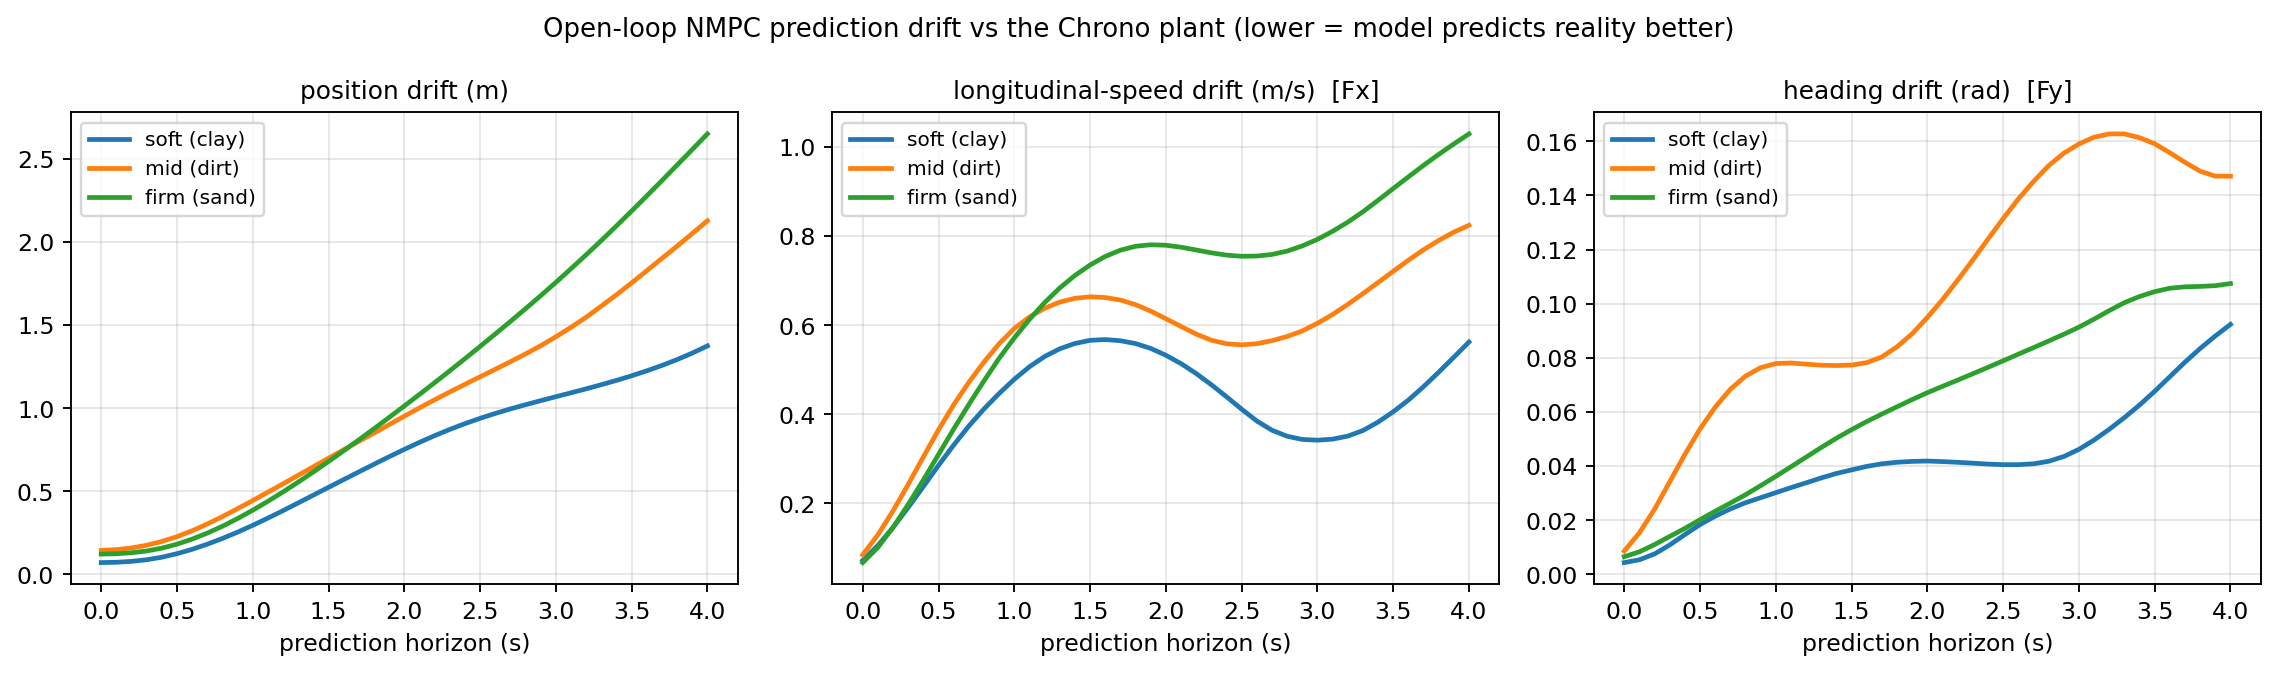
\includegraphics[width=\textwidth]{rollout_prediction_validation.png}
  \caption{Open-loop NMPC prediction drift versus the Chrono plant, by
    horizon time and terrain (mean over 18 runs, deployed vehicle-rate
    surrogate). Left: front-axle position drift. Middle: longitudinal-speed
    drift --- the deployment measure of $F_x$ prediction quality. Right:
    heading drift (lateral, $F_y$). The model predicts heading well
    ($\le 0.15\,$rad over $4\,$s) but carries a persistent
    ${\approx}0.5\,$m/s speed bias, so $F_x$ is the dominant prediction
    error.}
  \label{fig:pred_validation}
\end{figure*}

\subsection{Feature headroom and the structural force-prediction floor}
\label{sec:feature_headroom}
Section~\ref{sec:pred_validation} isolates $F_x$ as the dominant
prediction error. We test directly whether that gap, and the companion
rear-axle $F_y$ weakness, is closable with additional \emph{causal,
MPC-available} input features. Holding the deployed per-axle surrogate
architecture fixed ($64\!\times\!32$ tanh, scenario split, three seeds),
we retrain it with progressively richer inputs --- body-frame lateral
velocity $v$, yaw rate $\omega$, road-wheel angle $\delta$, a kinematic
lateral-load-transfer estimate, and their first differences --- and
report held-out RMSE per axle (Table~\ref{tab:feature_headroom}). IMU
accelerations are excluded as force consequences (label leakage).

The response is sharply asymmetric. Front-axle lateral force improves by
$14\%$ once the dynamic state and its rates are supplied: $F_{y,f}$
genuinely benefits from richer vehicle context. The longitudinal channel
is already at its feature floor --- $F_x$ RMSE falls at most $3\%$ on
either axle --- which
confirms the Section~\ref{sec:pred_validation} diagnosis at the model
level: the soft-soil speed bias is a dynamics-level motion-resistance
term, not a missing tire-model feature, and is therefore exactly the
bias the throttle disturbance observer
(Section~\ref{sec:throttledob}) absorbs online rather than something a
richer surrogate could learn away.

Rear-axle $F_y$ is a genuine structural floor. Beyond the $4\%$ of
Table~\ref{tab:feature_headroom} we tested two further
physically-motivated hypotheses on dedicated data, and neither moved it.
First, per-wheel \emph{sinkage}: because the rear wheels run on soil the
front has just compacted, the rear sinks markedly deeper (roughly $50\%$
deeper than the front in a controlled probe), so multi-pass soil state
is a plausible missing input; yet adding it improves rear $F_y$ by
$\le 3\%$ \emph{even when the surrogate is handed the ground-truth SCM
sinkage as an oracle}. Second, a $0.32$\,s causal history of the slip
and dynamic-state channels (a tire-relaxation hypothesis) yields $0\%$.
The rear lateral force is thus irreducible from MPC-available signals at
the deployed capacity; we treat it as a characterized limit
(Section~\ref{sec:limitations}), not a tuning target.

\begin{table}[!t]
  \renewcommand{\arraystretch}{1.15}
  \caption{Per-axle held-out force RMSE (N) as causal, MPC-available
    dynamic features are added to the deployed per-axle rate surrogate
    (mean over three scenario-split seeds). Front $F_y$ improves $14\%$;
    $F_x$ sits at its feature floor ($\le 3\%$) and rear $F_y$ barely moves
    ($4\%$), the structural limit characterized in the text.}
  \label{tab:feature_headroom}
  \centering
  \setlength{\tabcolsep}{5pt}
  \begin{tabular}{lcccc}
    \toprule
    & \multicolumn{2}{c}{\textbf{$F_x$ (N)}} & \multicolumn{2}{c}{\textbf{$F_y$ (N)}}\\
    \cmidrule(lr){2-3}\cmidrule(lr){4-5}
    \textbf{Surrogate inputs} & front & rear & front & rear\\
    \midrule
    Deployed (rate)            & 433 & 579 & 377 & 444\\
    {}\;+ dynamic state \& rates & 419 & 573 & \textbf{326} & 429\\
    \midrule
    Change                     & $-3\%$ & $-1\%$ & $\mathbf{-14\%}$ & $-4\%$\\
    \bottomrule
  \end{tabular}
\end{table}

%======================================================================
\section{Online Terrain Estimator}
\label{sec:estimator}
%======================================================================

The deployed terrain estimator fuses two complementary measurements of
the soil firmness inside a state-augmented UKF (Sec.~\ref{sec:ukf}): a
learned tire-force channel and a proprioceptive vibration channel. This
section introduces the proprioceptive channel --- a sliding-window MLP
--- and characterises its closed-loop convergence in isolation;
Sec.~\ref{sec:ukf} then shows why the force channel alone is blind to
firm soil and how the covariance-weighted fusion of the two restores
observability.

The proprioceptive MLP estimates the Bekker sinkage exponent
online from a 4-second window of 26 hand-crafted features over the
inertial and wheel-speed streams: speed mean/std/max; lateral and
longitudinal acceleration std and high percentiles; wheel-slip
mean/std/p95; lateral-grip and yaw-gain proxies; longitudinal drag;
mean steering magnitude and p95; throttle mean; and a vertical-dynamics
block of vertical-acceleration std/p95, pitch-rate std/p95, and
roll-rate std (motivated by Buzhardt~\&~Tallapragada~2024, whose
half-car UKF showed the suspension oscillation signature carries
strong Bekker-$n$ information). Every input is available from the
simulated onboard sensor stack (IMU, fused body velocity, steering
encoder, wheel encoders, commanded throttle); neither SCM tire forces
nor true terrain labels are read at inference time.

The MLP channel outputs $\hat n$ (and, in the heteroscedastic variant
the Fused-UKF consumes, a per-sample uncertainty $\sigma_{\mathrm{MLP}}$;
Sec.~\ref{sec:ukf}). Each controller tick
appends the newest sample to a rolling buffer; once a 4-second window
is filled, the feature vector is normalised by the training-set
scaler, passed through the MLP, clipped to the trained support, and
smoothed by an exponential moving average. The MPC starts from a
neutral dirt prior ($n\!=\!0.7$), accepts an estimator update about
$4.2\,\mathrm{s}$ into a run, and maps the smoothed $\hat n$ onto
$(K_\phi,K_c,c,\phi,k)$ by interpolation along the retained
clay--dirt--sand terrain manifold. The controller and safety filter
therefore receive a complete soil-parameter vector, but the live
identified degree of freedom in this paper is $n$ only.

\subsection{Closed-loop convergence}
\label{sec:estimator_convergence}

The proprioceptive MLP was trained on a broad multi-axis sweep of 3600
LHS-sampled SCM scenarios spanning $n\in[0.40,1.30]$ (180 cells), under
both scripted open-loop excitation and closed-loop NMPC tracking at
three target speeds ($4,6,8\,\mathrm{m/s}$) and three reference paths
(sinusoidal, lane-change, double-lane-change). With the channel
running inside the NMPC at the $10\,\mathrm{Hz}$ control rate,
the deployment-mode benchmark drives the same MPC stack across the
three canonical soils and six Bekker-jittered out-of-distribution
terrains (the five non-$n$ soil parameters perturbed
$\pm 30\text{--}50\,\%$ off the clay--dirt--sand interpolation
manifold), each under closed-loop NMPC sinusoidal tracking at
$v_{\mathrm{cmd}}\!\in\!\{5,7\}\,\mathrm{m/s}$, bumpiness $\in\{0,4\}$,
five seeds ($60$ in-distribution and $120$ OOD runs).

Table~\ref{tab:estimator_pilot} summarises the tail-window error: the
proprioceptive channel converges to mean $|\Delta n|=0.069$ (median
$0.066$) on the canonical soils and holds $0.081$ (median $0.071$)
across the OOD terrains. Its largest residual is on soft clay, whose
very low-$K_\phi$ response is read slightly upward toward the dirt
manifold (tail-mean estimate $0.59$ vs.\ true $0.50$,
Fig.~\ref{fig:estimator_scatter}) --- the well-known clay/dirt
$n$-ambiguity. This is exactly the regime where the Fused-UKF's
lateral-force channel adds complementary information
(Sec.~\ref{sec:ukf}).

\begin{table}[!t]
  \renewcommand{\arraystretch}{1.10}
  \caption{Proprioceptive (window-MLP) channel accuracy, evaluated
    \emph{within its training envelope} (bumpiness $\in\{0,4\}$; see
    Sec.~\ref{sec:training_data} and the OOD note below) under
    closed-loop NMPC sinusoidal tracking
    ($v_{\mathrm{cmd}}\in\{5,7\}\,\mathrm{m/s}$, $5$ seeds).
    In-distribution = the three canonical presets (clay/dirt/sand);
    random soils = Bekker-jittered OOD soils. $|\Delta n|$ is the
    tail-window absolute error (last 25\,\% of the active driving
    window). This is the proprioceptive channel alone; the deployed
    Fused-UKF that consumes it is benchmarked in Sec.~\ref{sec:ukf}.}
  \label{tab:estimator_pilot}
  \centering
  \begin{tabular}{lccc}
    \toprule
    \textbf{Set} & \textbf{Runs} &
    \textbf{$|\Delta n|$ mean} & \textbf{$|\Delta n|$ median}\\
    \midrule
    In-distribution    & $60$  & $0.069$ & $0.066$\\
    Random (OOD) soils & $120$ & $0.081$ & $0.071$\\
    \bottomrule
  \end{tabular}
\end{table}

\begin{figure}[!t]
  \centering
  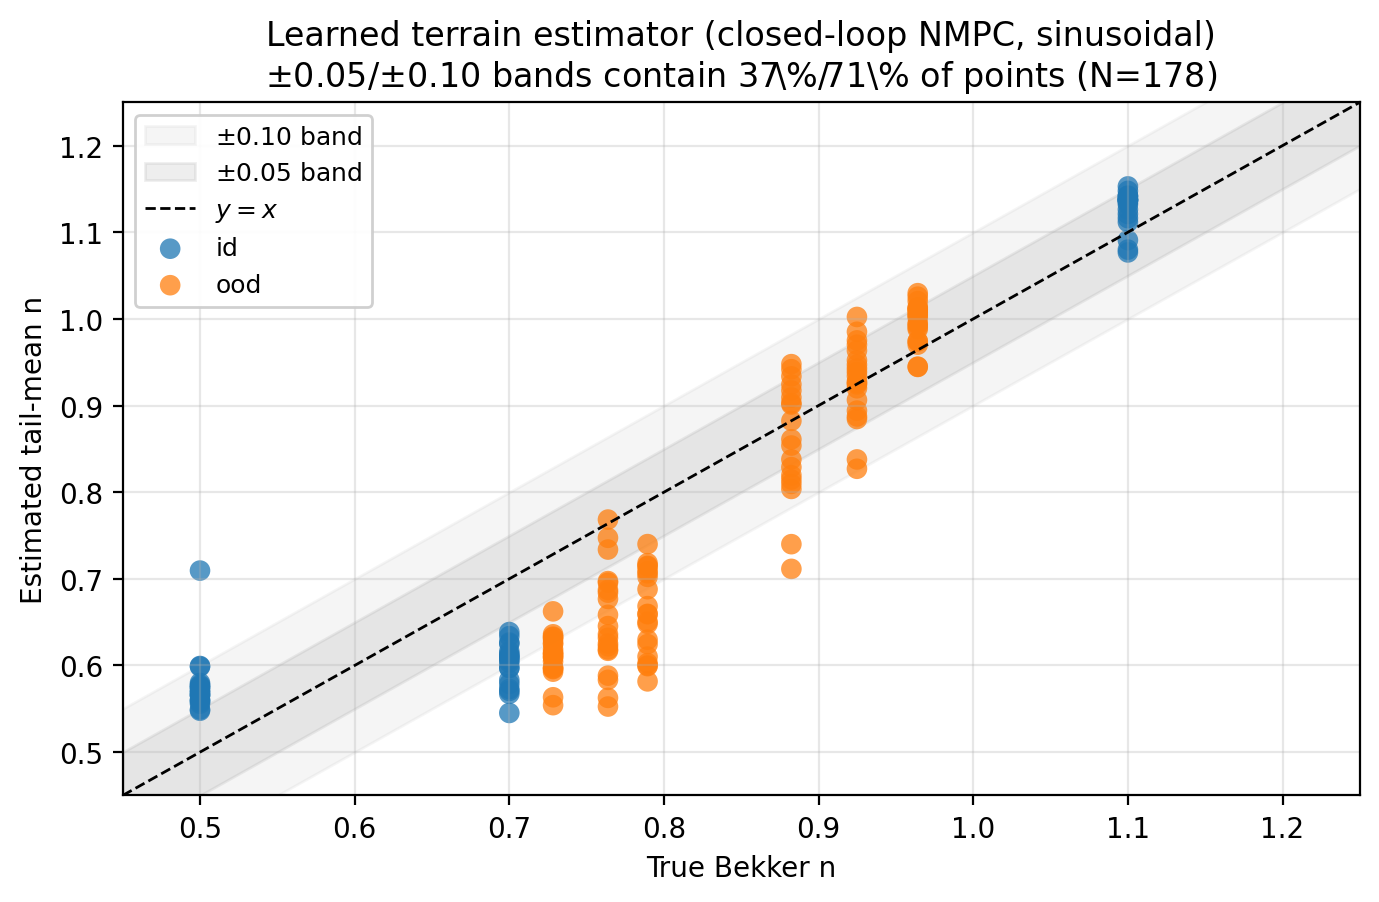
\includegraphics[width=\columnwidth]{terrain_estimator_scatter.png}
  \caption{Learned (sliding-window MLP) terrain estimator: true vs.\
    estimated Bekker $n$ (tail-window mean) on the closed-loop
    sinusoidal benchmark, evaluated \emph{within the estimator's
    training envelope} (bumpiness $\in\{0,4\}$). Blue = in-distribution
    canonical soils (clay/dirt/sand); orange = Bekker-jittered
    out-of-distribution soils ($n$ sampled in $[0.40,1.30]$, other five
    Bekker parameters perturbed $\pm 30\text{--}50\,\%$). The
    $\pm 0.05$ / $\pm 0.10$ bands around $y=x$ contain $40\,\%$ / $68\,\%$
    of points. The estimator tracks the diagonal across the deployment
    range, with a mild systematic over-prediction in the lowest-$n$
    (clay) bin (mean estimate $0.59$ vs.\ true $0.50$). See the
    out-of-envelope note in the text for behaviour at bumpiness $8$.}
  \label{fig:estimator_scatter}
\end{figure}

\begin{figure}[!t]
  \centering
  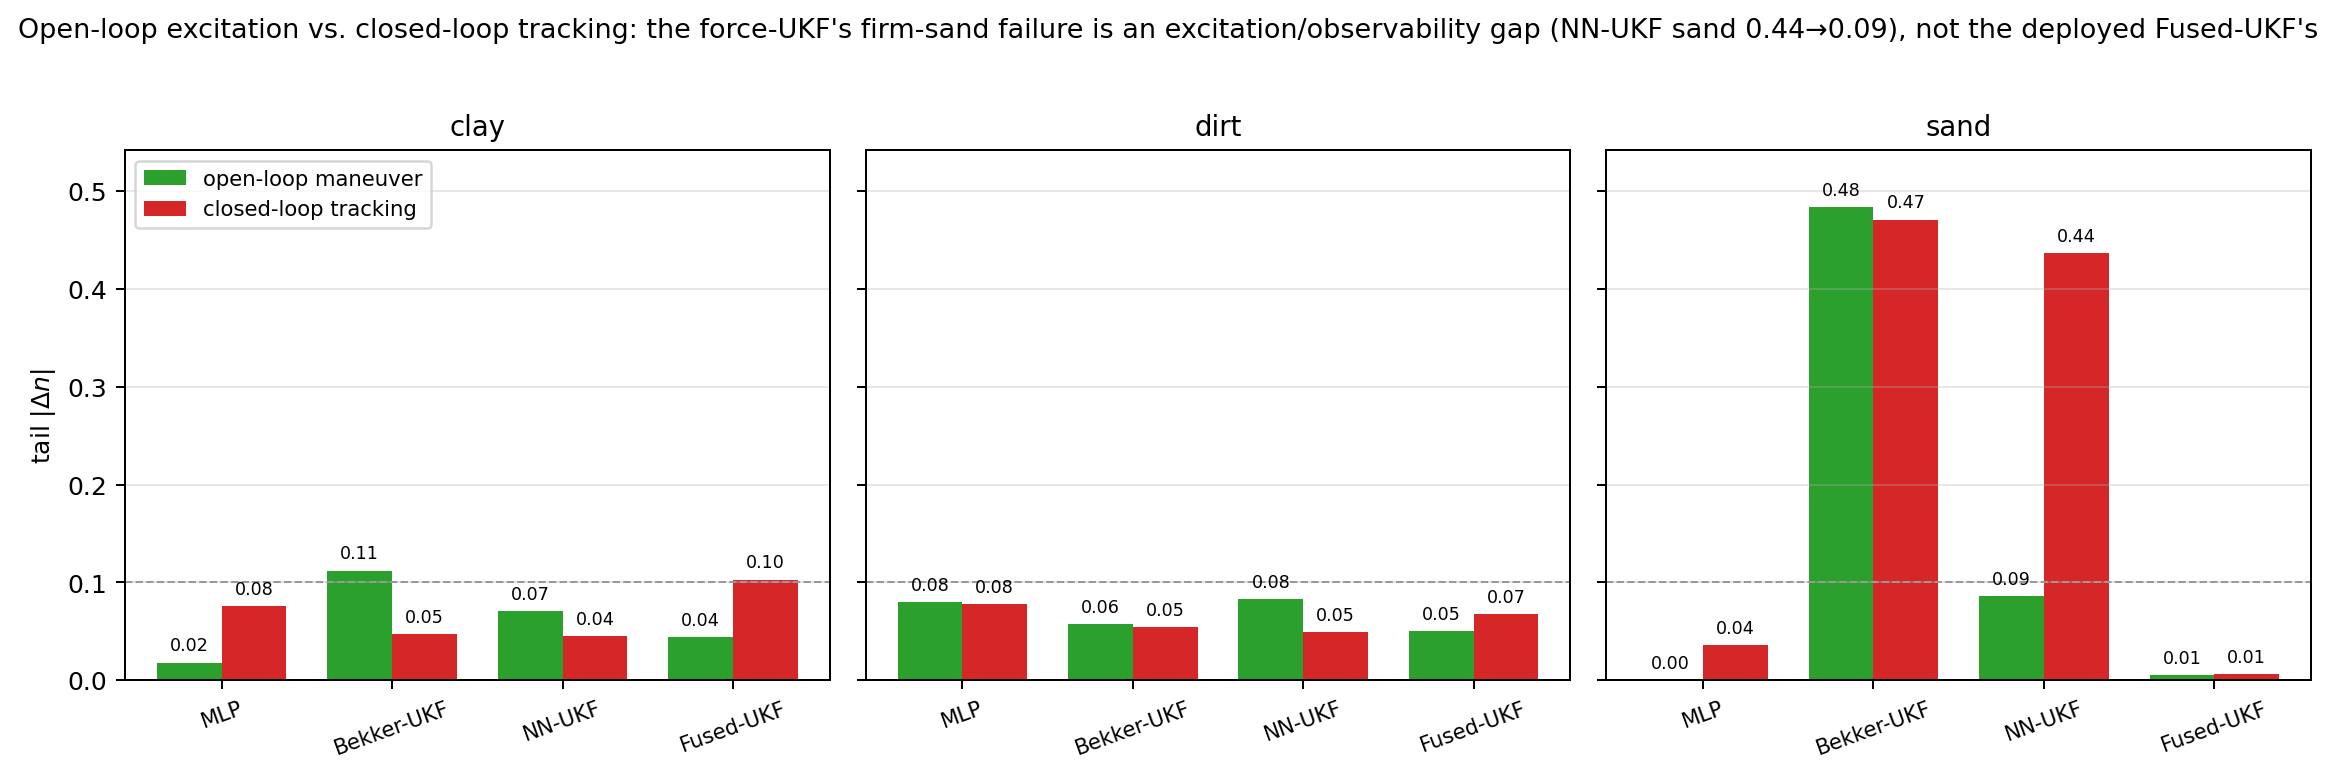
\includegraphics[width=\columnwidth]{open_loop_estimator_diagnostic.png}
  \caption{Open-loop excitation vs.\ closed-loop tracking, all four
    estimators, canonical soils (tail $|\Delta n|$). A scripted
    $0.6\,$rad sine-steer maneuver (green) is compared to closed-loop
    NMPC path-tracking (red). On firm sand the force-only NN-UKF goes
    $0.44\!\to\!0.09$ --- \emph{observability}-limited, a dedicated maneuver
    resolves it --- whereas the Bekker-UKF remains $\approx\!0.47$ in both
    (\emph{model}-limited: its analytical contact law is inaccurate on sand).
    The proprioceptive MLP is excitation-agnostic ($0.04\!\to\!0.00$),
    and the deployed Fused-UKF is accurate in both ($\approx\!0.01$),
    so it needs no dedicated maneuver at runtime
    (cf.\ Sec.~\ref{sec:ukf}).}
  \label{fig:estimator_open_loop}
\end{figure}

\paragraph{Out-of-envelope behaviour (bumpiness).}
The learned estimator's window features include a vertical-dynamics
block ($a_z$ and pitch/roll-rate statistics) that senses how strongly
the chassis rides over terrain undulation; these features were trained
only at bumpiness $\in\{0,4\}$ (Table~\ref{tab:training_data}). At
bumpiness $8$ --- outside that training envelope --- the bump-induced
vertical excitation is mis-read as firm-soil stiffness and the estimate
on soft clay diverges upward: the tail-mean estimate at $n=0.5$ rises
from $0.59$ in-envelope to $1.03$ ($|\Delta n|\!\approx\!0.53$), i.e.\
the estimator reports near-firm soil on the softest terrain. This is a
genuine out-of-distribution failure on the bumpiness axis, not a
low-$n$ failure per se --- clay is estimated accurately
($|\Delta n|\!\approx\!0.09$) at bumpiness $\le 4$. It is a limitation
of the deployed window-MLP, not of the framework: the state-augmented
NN-UKF of Sec.~\ref{sec:ukf} infers $n$ through a physics-based bicycle
model and does not show this bumpiness sensitivity. Extending the
estimator's training set to higher bumpiness, or gating the
vertical-dynamics features on an online road-roughness estimate, would
close the gap; we report the in-envelope result here and flag the
extrapolation regime explicitly rather than averaging over it.

\subsection{Closed-loop terrain estimation: force observability and a proprioceptive-fused UKF}
\label{sec:estimator_ukf}
\label{sec:ukf}

The deployed terrain estimator is a \textbf{Fused-UKF}: a
state-augmented unscented Kalman filter that, following the
state-augmentation idea of Dallas et al.~\cite{Dallas21}, estimates
the Bekker sinkage exponent $n$ jointly with the bicycle state, but
fuses \emph{two} measurement channels of $n$ rather than one.
\textbf{(i)} A whole-vehicle lateral-force channel: a learned surrogate
maps the bicycle's own state plus the six Bekker--Mohr soil parameters
to $(F_{y,\mathrm{total}}, M_{\mathrm{yaw,total}})$, and the UKF
observes the body-frame $a_y$ as a direct measurement of
$\Sigma F_y/m$. \textbf{(ii)} A proprioceptive channel: the deployed
\emph{heteroscedastic} sliding-window MLP supplies an independent
measurement $n_{\mathrm{MLP}}$ \emph{together with} its own per-sample
uncertainty $\sigma_{\mathrm{MLP}}$, which the UKF consumes as the
proprioceptive measurement noise $R_n$. The full measurement vector is
$[x,y,\psi,u,v,\omega,\,a_y,\,n_{\mathrm{MLP}}]^\top$, and the two
$n$-channels are weighted purely by Kalman covariance --- there is
\emph{no} hand-tuned gate or external blend. The MLP is trained with a
Gaussian negative-log-likelihood objective (val RMSE$_n$ $0.064$;
$\mathrm{corr}(|\mathrm{err}|,\sigma_{\mathrm{MLP}})\!=\!0.71$), so it
reports low $\sigma$ exactly where it is accurate --- notably on firm
sand --- and the filter automatically trusts it there.

We compare the deployed Fused-UKF against two force-only baselines that
share the identical UKF and bicycle but drop the proprioceptive
channel: \textbf{(i) Bekker-UKF}, an analytical Bekker--Wong
contact-patch integration that mirrors the SCM plant's own formulation,
and \textbf{(ii) NN-UKF (force-only)}, the whole-vehicle lateral-force
surrogate driving the prediction step with no proprioceptive
measurement. The bicycle is the 4-wheel double-track variant of
Dallas's 3-DOF model --- each wheel receives its own vertical load
under quasi-static longitudinal and lateral transfer driven by measured
$a_x$, $a_y$, the steering input, and the body-frame yaw rate.

\paragraph{Whole-vehicle lateral-force surrogate.} Earlier iterations
trained the UKF's NN on a single-tyre rig (paper118 protocol) and
wrapped it in a hand-tuned rig-to-vehicle gain
($1.15\times$ on $F_y$) to close the $\approx 15\,\%$ gap between
single-tyre rig forces and full-suspension HMMWV forces. The
calibration was acceptable at the two soft-soil presets paper118
reported but did not generalise to a broad LHS sweep, so we replaced
it with a surrogate that natively predicts what the *whole vehicle*
produces:
\[
  \resizebox{\columnwidth}{!}{$\displaystyle
  \mathrm{NN}_{F_y}\!:\, (u, v, \omega, \delta, K_\phi, K_c, n,
  c, \phi, k)\ \mapsto\ (F_{y,\mathrm{total}},\ M_{\mathrm{yaw,total}})$}.
\]
The surrogate is a 128–64 ReLU MLP trained on a 300-sample,
9-axis uniform LHS sweep
(seed 7)
that varies the six Bekker--Mohr soil parameters together with three
maneuver axes — steering amplitude $0.20\text{--}0.65\,$rad,
steering period $2\text{--}5\,$s, and target cruise speed
$3.5\text{--}7\,$m/s (half the runs use constant open-loop throttle,
half a PI cruise) — yielding $\approx 190\,000$ labelled rows.
Crucially, the soil axes are sampled from a \emph{widened} box
($K_\phi$ from $0.3\,$MPa, cohesion from $300\,$Pa, Janosi shear
$0.008\text{--}0.028\,$m, $n\in[0.35,1.35]$): the canonical clay,
dirt and sand presets sit on the \emph{edges} of the deployed
\texttt{TRAINING\_RANGES\_V6} box (clay's $K_\phi$ is at $5\,\%$ of
range and its Janosi shear at the $0\,\%$ floor), so a surrogate
trained on that box has to extrapolate to reach them and fails on
clay. Widening the box (never narrowing — CLAUDE.md §8) turns those
soils into interior points the surrogate interpolates to.
Targets are extracted directly from each Chrono log:
$F_{y,\mathrm{total}}\!=\!m\,a_y$ and
$M_{\mathrm{yaw,total}}\!=\!I_z\,\dot\omega$ (5-point central
difference). Held-out (30 of 300 scenarios, scenario-split) $R^2$ is
$0.90$ on $F_y$ and $0.88$ on $M_{\mathrm{yaw}}$. CLAUDE.md §8 holds:
every input axis is uniformly sampled over its (widened) box, with
no narrowing toward a canonical preset or controller-conditioned
operating point, and the trained model is plugged into the UKF
\emph{without} any per-soil scalar correction. This surrogate is the
UKF's force channel for both the Fused-UKF and the force-only NN-UKF.

\paragraph{Force observability of $n$ (the key issue).}
The reason the force channel alone is not enough is an
\emph{observability} gap, not a model defect. Under a path-tracking
controller the slip stays small, and at that operating point the
lateral force carries almost no information about $n$ on firm soil. At
a representative small-slip operating point the lateral-force signal
separating firm from soft soil is
$|F_y(n\!=\!1.1)-F_y(n\!=\!0.7)|\!\approx\!132\,$N, well below the
lateral-accel measurement-noise floor of
$\approx\!770\,$N ($=m\,R_{a_y}$ with $R_{a_y}\!=\!0.3\,$m/s$^2$). Under
a \emph{scripted} $0.6\,$rad steering maneuver the same delta grows to
$743\,$N --- at the noise floor --- and $\mathrm{d}F_y/\mathrm{d}n$ is
$\approx\!16\times$ larger. The yaw channel is worse still:
$|\mathrm{d}M_z|\,\Delta n\!\approx\!191\,$N$\cdot$m sits below its
$\approx\!216\,$N$\cdot$m noise floor and stays unobservable even at
large slip. A force-only UKF is therefore \emph{blind} to firm-soil $n$
under gentle tracking: the signal it would need to correct $n$ is
buried in the measurement noise. Fig.~\ref{fig:ukf_observability}
makes this concrete --- and shows that the proprioceptive channel,
which reads vibration rather than slip-dependent force, fills exactly
this gap.

\begin{figure}[!t]
  \centering
  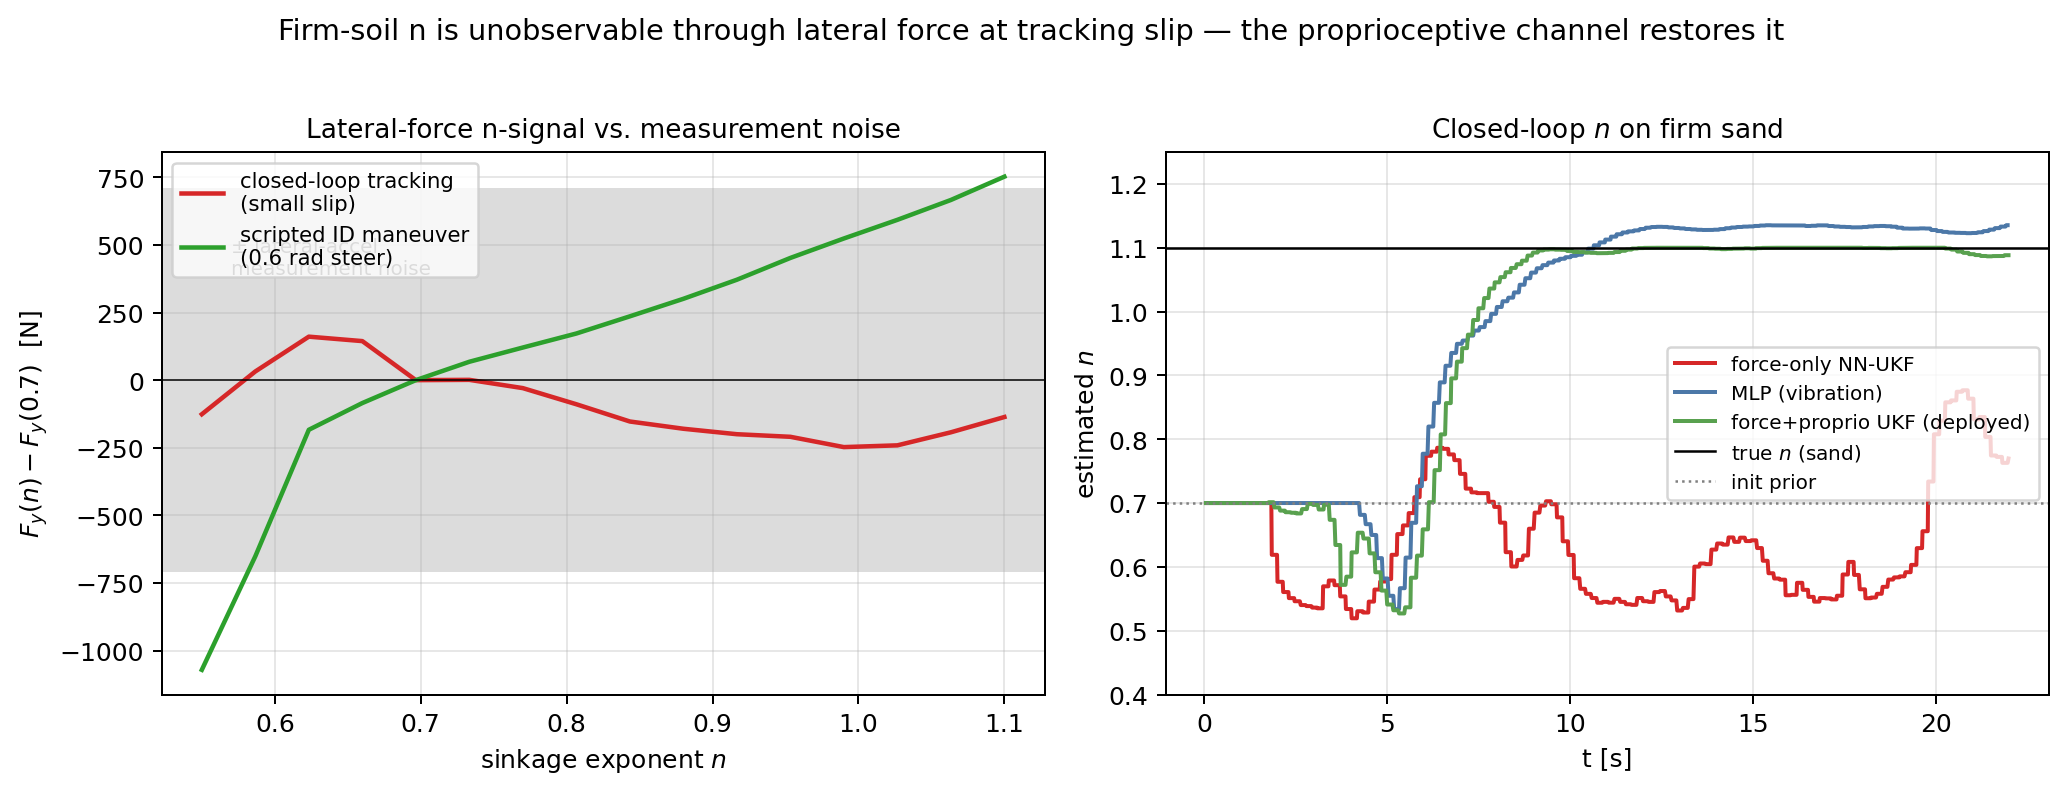
\includegraphics[width=\columnwidth]{ukf_observability.png}
  \caption{Force observability of the sinkage exponent $n$.
    \textbf{Left:} the lateral-force $n$-signal
    $|F_y(n\!=\!1.1)-F_y(n\!=\!0.7)|$ against the lateral-accel
    measurement-noise band ($m\,R_{a_y}\!\approx\!770\,$N,
    $R_{a_y}\!=\!0.3\,$m/s$^2$). At closed-loop small-slip path
    tracking the signal ($\approx\!132\,$N) stays \emph{inside} the
    band --- $n$ is unobservable from force --- whereas a scripted
    $0.6\,$rad maneuver escapes it ($\approx\!743\,$N, with
    $\mathrm{d}F_y/\mathrm{d}n$ $\approx\!16\times$ larger). \textbf{Right:}
    closed-loop $\hat n(t)$ on firm sand: the force-only NN-UKF, lacking
    an observable force signal, drifts in the \emph{wrong} direction, while the
    deployed Fused-UKF tracks the true $n$ by leaning on its
    proprioceptive channel.}
  \label{fig:ukf_observability}
\end{figure}

\paragraph{Open-loop vs.\ closed-loop: two distinct failure modes.}
The earlier open-loop diagnostic (Fig.~\ref{fig:estimator_open_loop})
separates an \emph{observability} limit from a \emph{model} limit by
comparing each estimator's tail $|\Delta n|$ on firm sand under a
scripted excitation maneuver against the same soil under closed-loop
tracking. The force-only NN-UKF goes from $0.09$ (open-loop) to $0.44$
(closed-loop): it is observability-limited, and a dedicated excitation
maneuver \emph{resolves} it. The Bekker-UKF remains model-limited in both
($0.48\!\to\!0.47$): it is model-limited --- the analytical Bekker law
is inaccurate on sand, and no amount of excitation can compensate. The
proprioceptive MLP, which reads vibration and is excitation-agnostic,
is accurate in both ($0.00\!\to\!0.04$), and the Fused-UKF inherits that
robustness ($0.01\!\to\!0.01$). This is the observability story seen
from the other side, and it is why the deployed estimator needs
\emph{no} dedicated excitation maneuver at runtime.

\paragraph{The deployed Fused-UKF closes the gap (canonical presets).}
Fig.~\ref{fig:estimator_comparison} reports the four estimators run
\emph{live in the closed loop} on the canonical clay/dirt/sand presets
at $v\!\in\!\{5,7\}\,$m/s (three seeds each); all numbers are tail
$|\Delta n|$ (lower is better). The proprioceptive MLP gives clay
$0.076$, dirt $0.078$, sand $0.036$ (overall $0.063$); the Bekker-UKF
$0.047$, $0.054$, $0.471$ (overall $0.190$); the force-only NN-UKF
$0.045$, $0.049$, $0.437$ (overall $0.162$); and the deployed Fused-UKF
$0.103$, $0.068$, $0.006$ (overall $0.059$). The two force-only UKFs
collapse on firm sand ($\approx\!0.44\text{--}0.47$) for exactly the
observability reason above, whereas the proprioceptive channel makes
$n$ observable, so the Fused-UKF accurately recovers firm sand
($|\Delta n|\!=\!0.006$) and is the most accurate estimator overall
($0.059$). We note one limitation plainly: the Fused-UKF is the
\emph{least} accurate on canonical clay ($0.103$) --- both force-only
UKFs and the MLP outperform it there, because the proprioceptive
channel is slightly over-weighted on soft, on-manifold soil where the
force channel is already reliable. The trade is nonetheless favourable:
the deployed filter accepts a small clay penalty in exchange for
eliminating the firm-sand failure exhibited by both force-only
baselines.

\begin{figure*}[!t]
  \centering
  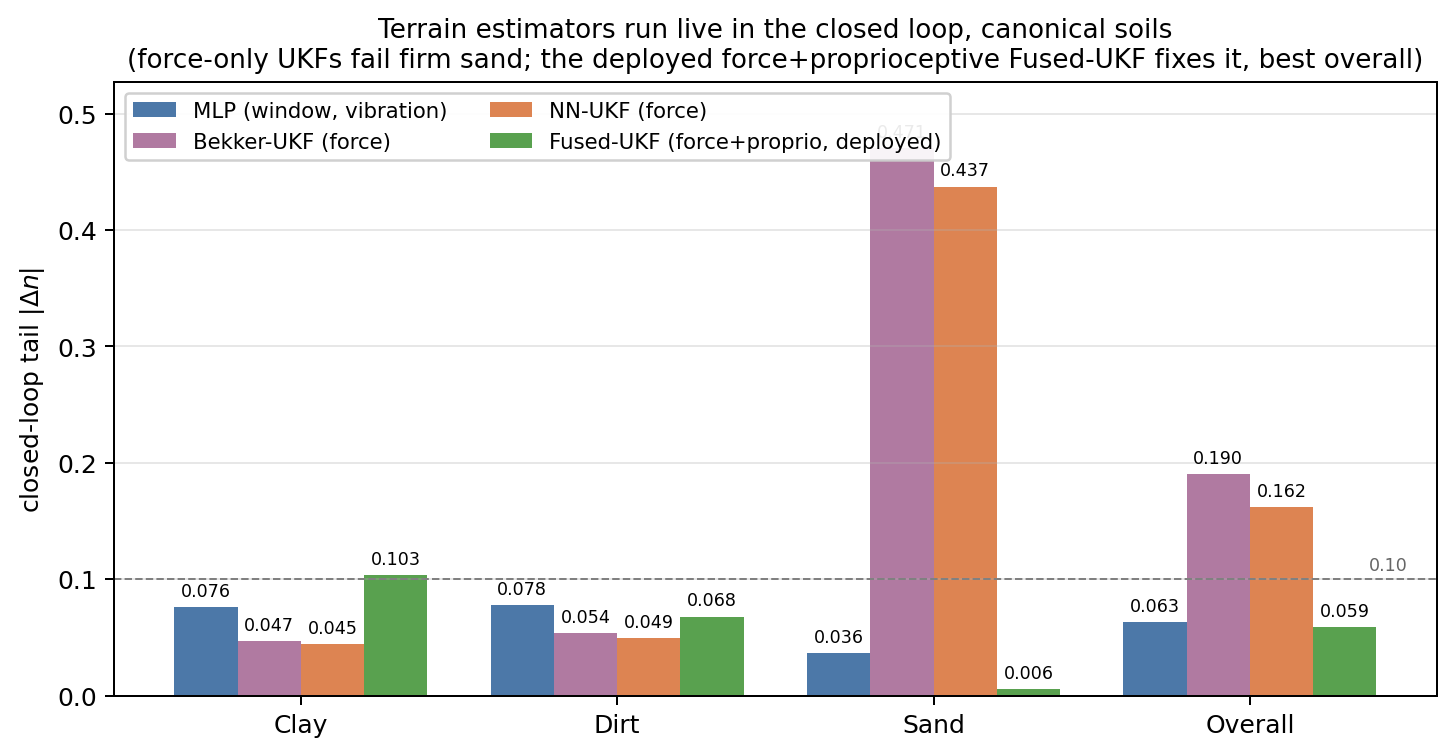
\includegraphics[width=\textwidth]{terrain_estimator_comparison.png}
  \caption{Per-terrain closed-loop comparison of the four estimators on
    the canonical Chrono SCM presets --- clay, sandy loam (dirt), dry
    sand --- run \emph{live} in the loop at $v\!\in\!\{5,7\}\,$m/s,
    three seeds, $0.6\,$rad steering, tail $|\Delta n|$. The Bekker-UKF
    and force-only NN-UKF are most accurate on the soft soils but fail
    on firm sand ($|\Delta n|\!\approx\!0.44\text{--}0.47$, an
    observability limit, cf.\ Fig.~\ref{fig:ukf_observability}); the
    proprioceptive MLP is balanced; the deployed Fused-UKF recovers firm
    sand to $0.006$ at the cost of being least accurate on soft clay
    ($0.103$).}
  \label{fig:estimator_comparison}
\end{figure*}

\begin{figure}[!t]
  \centering
  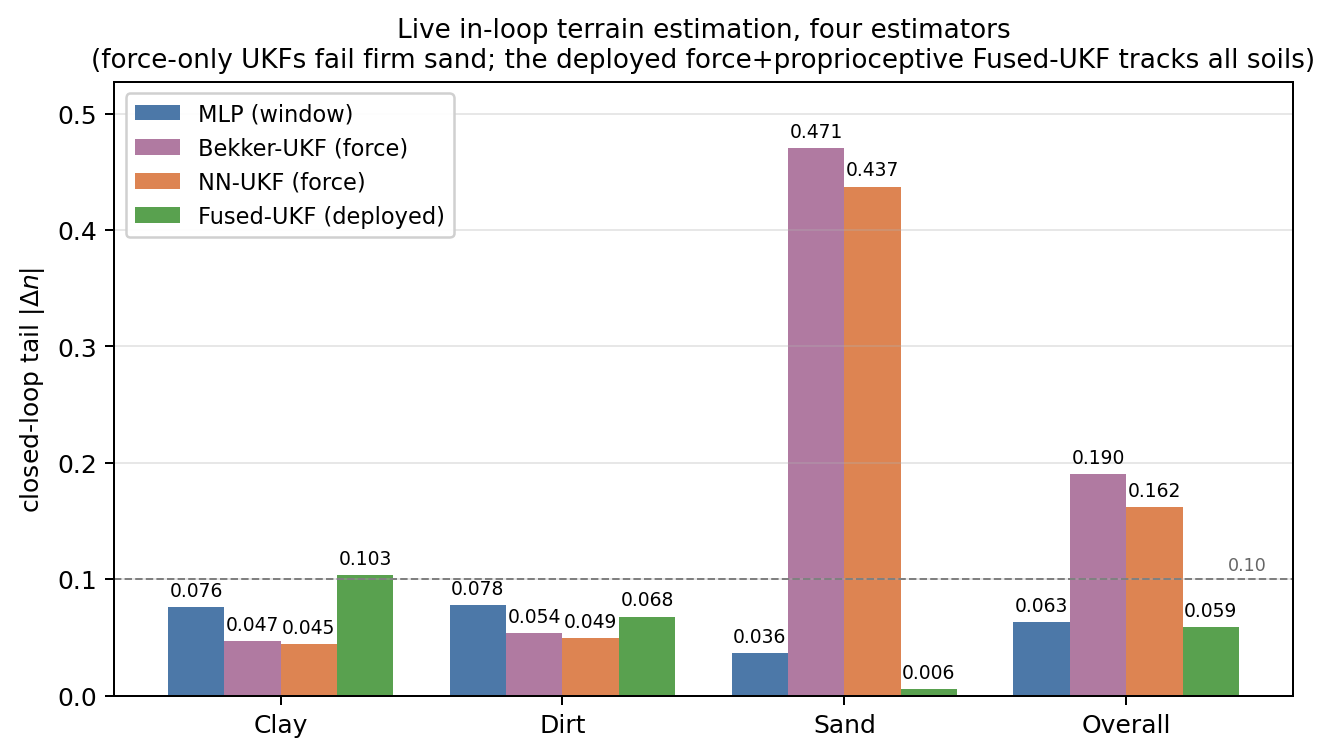
\includegraphics[width=\columnwidth]{closed_loop_estimator_backends.png}
  \caption{Deployment summary: tail $|\Delta n|$ over the canonical
    clay/dirt/sand presets and the overall mean for the proprioceptive
    MLP, the analytical Bekker-UKF, the force-only NN-UKF, and the
    deployed Fused-UKF (all run live in the closed loop,
    $v\!\in\!\{5,7\}\,$m/s, three seeds). The force-only UKFs fail firm
    sand; the covariance-fused proprioceptive channel makes $n$
    observable, so the Fused-UKF is best overall ($0.059$) with no
    hand-tuned gate.}
  \label{fig:cl_estimator_backends}
\end{figure}

\paragraph{Broad robustness across the deployable $n$ range.}
Fig.~\ref{fig:estimator_lhs100} and Table~\ref{tab:estimator_lhs100}
report the head-to-head on \textbf{100 soils swept along the canonical
clay--dirt--sand Bekker--Mohr manifold} (seed 42,
$n\!\in\![0.52,1.08]$; the other five soil parameters follow the preset
manifold with $\pm 8\,\%$ jitter --- the parameter-known setting in
which the force-dominant exponent $n$ is isolated, and the soil model
the estimator reconstructs from $\hat n$), \emph{all} run live
closed-loop under NMPC sinusoidal path-tracking at $5\,$m/s. The
deployed Fused-UKF and the proprioceptive MLP recover $n$ across the
full range (median error $4.5\,\%$ and $6.7\,\%$; $94\,\%$ and
$83\,\%$ within $\pm 20\,\%$), their estimates tracking the diagonal.
The force-only NN-UKF and Bekker-UKF instead saturate near
$n\!\approx\!0.6$ on firm soils ($23.8\,\%$ median error): without a
proprioceptive channel they cannot observe $n$ once closed-loop slip is
small --- the force-observability limit of Sec.~\ref{sec:ukf}, now
visible across the whole sweep rather than only on canonical sand. The
deployed Fused-UKF leads every metric (Fig.~\ref{fig:estimator_overall}).

\begin{figure*}[!t]
  \centering
  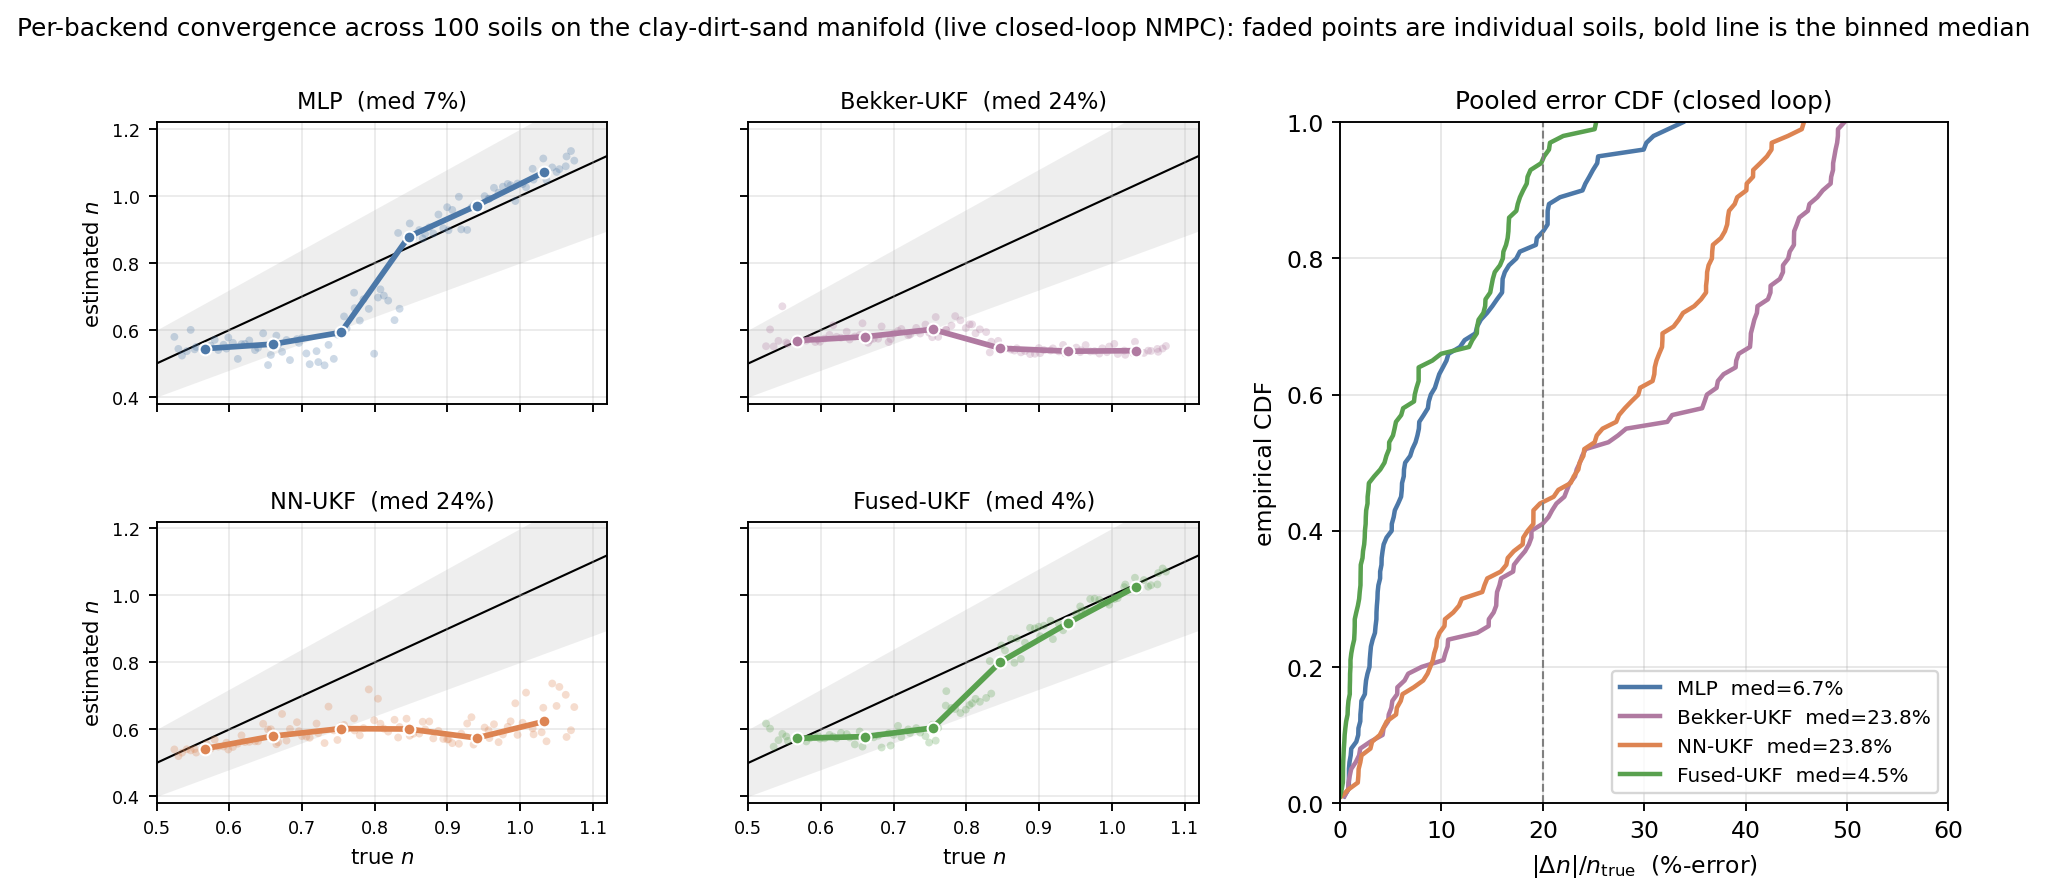
\includegraphics[width=\textwidth]{lhs100_fair.png}
  \caption{Closed-loop terrain-estimator benchmark on 100 soils swept
    along the clay--dirt--sand Bekker--Mohr manifold in Chrono SCM
    (seed 42, $n\!\in\![0.52,1.08]$; the other five soil parameters
    follow the preset manifold with $\pm 8\,\%$ jitter --- the
    parameter-known setting in which the force-dominant exponent $n$ is
    estimated, and the soil model our estimator reconstructs from
    $\hat n$), all run live under closed-loop NMPC sinusoidal
    path-tracking at $5\,$m/s. Left, four panels: estimated $n$ versus
    true $n$ per backend, where faded points are individual soils, the
    bold line is the binned median, and the black diagonal with its
    $\pm 20\,\%$ band is the target. The proprioceptive MLP and the
    deployed Fused-UKF track the diagonal (fitted slope $1.25$ and
    $1.07$), whereas the force-only NN-UKF and Bekker-UKF saturate near
    $n\!\approx\!0.6$ on firm soils (slope $0.15$ and $-0.11$) --- the
    closed-loop force-observability limit quantified in
    Sec.~\ref{sec:ukf}. Right: pooled empirical CDF of the tail-window
    $|\Delta n|/n_{\mathrm{true}}$; the Fused-UKF holds the tightest
    distribution and the best fraction within $\pm 20\,\%$ (dashed
    line).}
  \label{fig:estimator_lhs100}
\end{figure*}

\begin{table}[!t]
  \renewcommand{\arraystretch}{1.10}
  \caption{Closed-loop terrain-estimator head-to-head on 100 soils
    swept along the clay--dirt--sand Bekker--Mohr manifold
    ($n\!\in\![0.52, 1.08]$, seed 42), all run live under closed-loop
    NMPC sinusoidal path-tracking at $5\,$m/s. The other five soil
    parameters follow the preset manifold ($\pm 8\,\%$ jitter), the
    parameter-known setting for isolating the force-dominant exponent
    $n$. Errors are tail-window $|\Delta n|$ (absolute) and
    $|\Delta n|/n_{\mathrm{true}}$ (relative). The deployed Fused-UKF
    row is bold.}
  \label{tab:estimator_lhs100}
  \centering
  \begin{tabular}{lccc}
    \toprule
    \textbf{Estimator} & median $|\Delta n|$ & median \%err
        & within $\pm20\,\%$\\
    \midrule
    MLP        & $0.055$ & $6.7\,\%$  & $83\,\%$\\
    Bekker-UKF & $0.189$ & $23.8\,\%$ & $41\,\%$\\
    NN-UKF     & $0.186$ & $23.8\,\%$ & $44\,\%$\\
    \textbf{Fused-UKF} & $\mathbf{0.028}$ & $\mathbf{4.5\,\%}$
        & $\mathbf{94\,\%}$\\
    \bottomrule
  \end{tabular}
\end{table}

\begin{figure*}[!t]
  \centering
  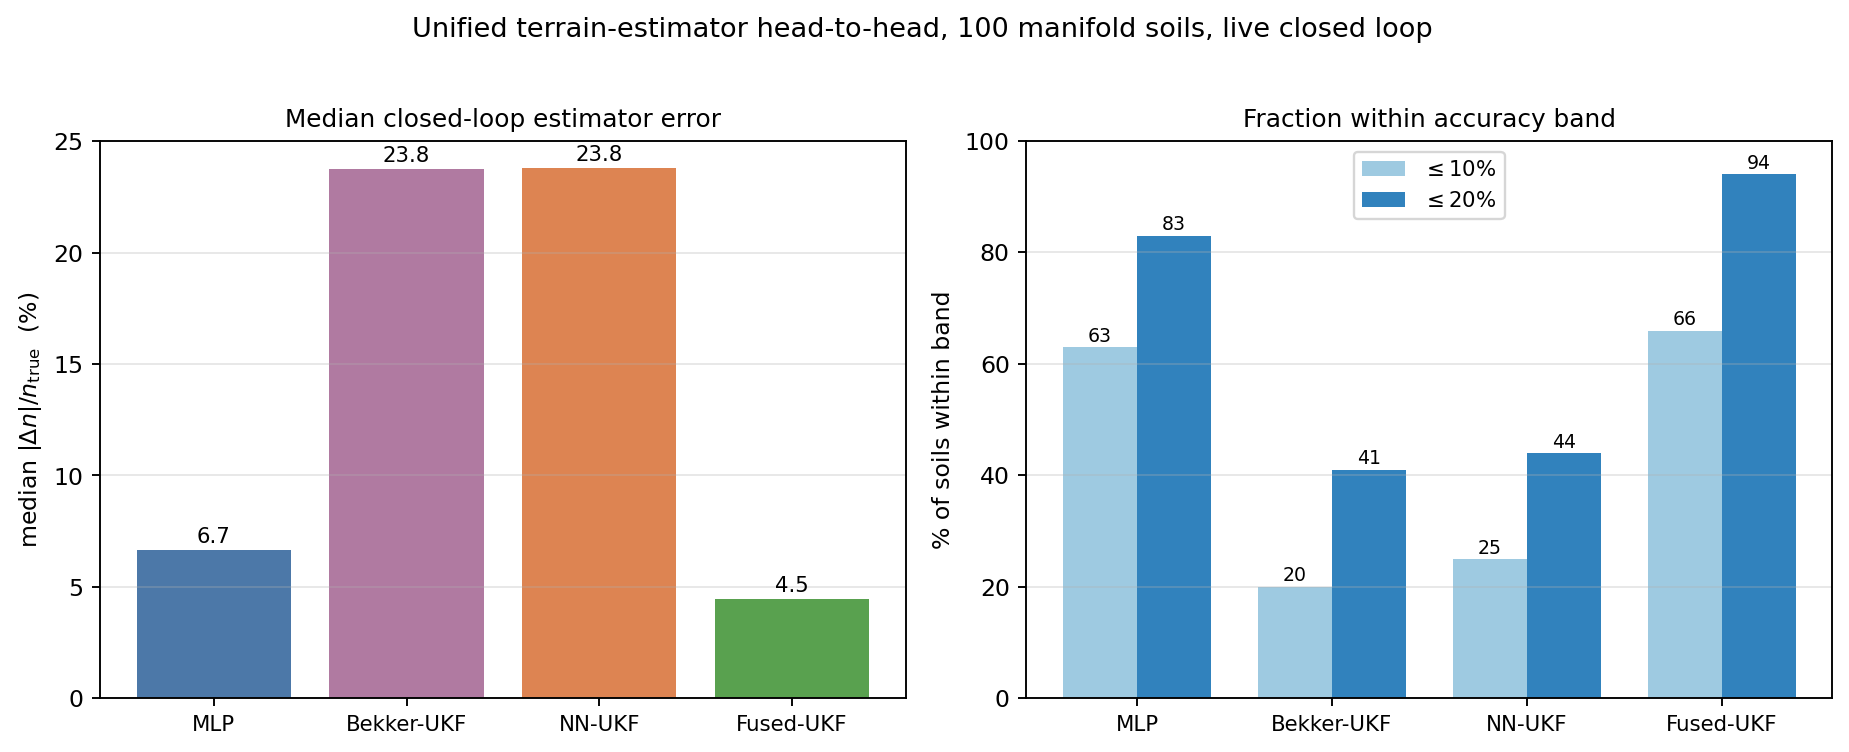
\includegraphics[width=\textwidth]{estimator_overall.png}
  \caption{Pooled closed-loop terrain-estimator comparison over the 100
    manifold soils. \textbf{Left:} median $|\Delta n|/n_{\mathrm{true}}$.
    \textbf{Right:} fraction within the $\pm 10\,\%$ / $\pm 20\,\%$
    bands. The deployed Fused-UKF is the most accurate ($94\,\%$ within
    $\pm 20\,\%$) and the MLP second ($83\,\%$); the force-only NN-UKF
    and Bekker-UKF trail because they cannot observe $n$ on firm soils
    in closed loop, with no hand-tuned gate needed in the Fused-UKF.}
  \label{fig:estimator_overall}
\end{figure*}

%======================================================================
\section{Terrain-Aware Speed Planning}
\label{sec:speedplan}
%======================================================================

The reference-tracking NMPC follows a speed reference $v_{\mathrm{ref}}(s)$
along the path. A purely geometric curvature-limited profile
($v_{\mathrm{ref}}=\sqrt{a_{y,\max}/|\kappa(s)|}$ at a fixed $a_{y,\max}$)
is blind to the soil: on soft terrain it commands cornering speeds the
available grip cannot support, so the vehicle understeers off the line.
The failure is most visible on the high-speed sinusoid, exactly where the
analytical baselines of Sec.~\ref{sec:tires_static} pile up
(Fig.~\ref{fig:tires_static_heatmap}).

We replace it with a terrain-aware, quasi-steady-state time-optimal
profile over a friction-circle (g--g) budget. At each control step the
deployed tyre surrogate is queried at the live estimate $\hat n$ and the
per-axle vertical load for the available lateral force
($\!\to a_{y,\max}$) and tractive/braking force
($\!\to a_{x,\max},\,a_{x,\mathrm{brake}}$); a forward--backward pass then
returns the fastest $v_{\mathrm{ref}}(s)$ that keeps the combined demand
inside the circle,
\begin{equation}
  \Big(\tfrac{a_x}{a_{x,\max}}\Big)^{2}
  + \Big(\tfrac{v^{2}\,\kappa(s)}{a_{y,\max}}\Big)^{2} \le 1,
\end{equation}
with a grip-safety margin that de-rates the surrogate's peak-force query
to leave transient headroom. The curvature $\kappa(s)$ is read from the
analytic arc-length spline of the path rather than finite-differenced
over the horizon, whose node spacing varies with speed and otherwise
spikes $\kappa$ into spurious $v_{\mathrm{ref}}$ craters (``slowing for no
reason''). This is a third use of the differentiable surrogate, alongside
in-horizon force prediction and the traction-budget constraint: the same
model that lets the NMPC track also tells the planner how fast the soil
will let it corner.

A closed-loop A/B against the geometric reference (clay/dirt/sand
$\times$ \{sinusoid, double lane change\} $\times\,\{5,7\}\,\mathrm{m/s}$,
two seeds; Fig.~\ref{fig:speedplan}) cuts mean RMS CTE by $49\,\%$
($0.146\!\to\!0.075\,\mathrm{m}$) for a $7\,\%$ reduction in mean speed.
The gain concentrates on exactly the cells the curvature heuristic
over-drives --- the high-speed sinusoid on soft soil, where CTE falls by
$75$--$81\,\%$ (dirt $0.544\!\to\!0.135$, clay
$0.469\!\to\!0.088\,\mathrm{m}$) --- and is neutral on the already-benign
cells. The trade is grip-limited rather than tunable: raising the safety
margin to recover the lost speed buys little (on dirt at
$7\,\mathrm{m/s}$, $+0.3\,\mathrm{m/s}$) while tripling CTE
($0.10\!\to\!0.28\,\mathrm{m}$), so the operating point sits at the knee
of the speed/accuracy frontier. Because the profile reads its grip limits
from whichever tyre model the controller carries, the tire-model
comparison of Sec.~\ref{sec:tires_static} holds it fixed at the geometric
reference to isolate the tracking model; the system-level closed-loop
sweeps elsewhere in the paper run the deployed g--g profile.

\begin{figure*}[!t]
  \centering
  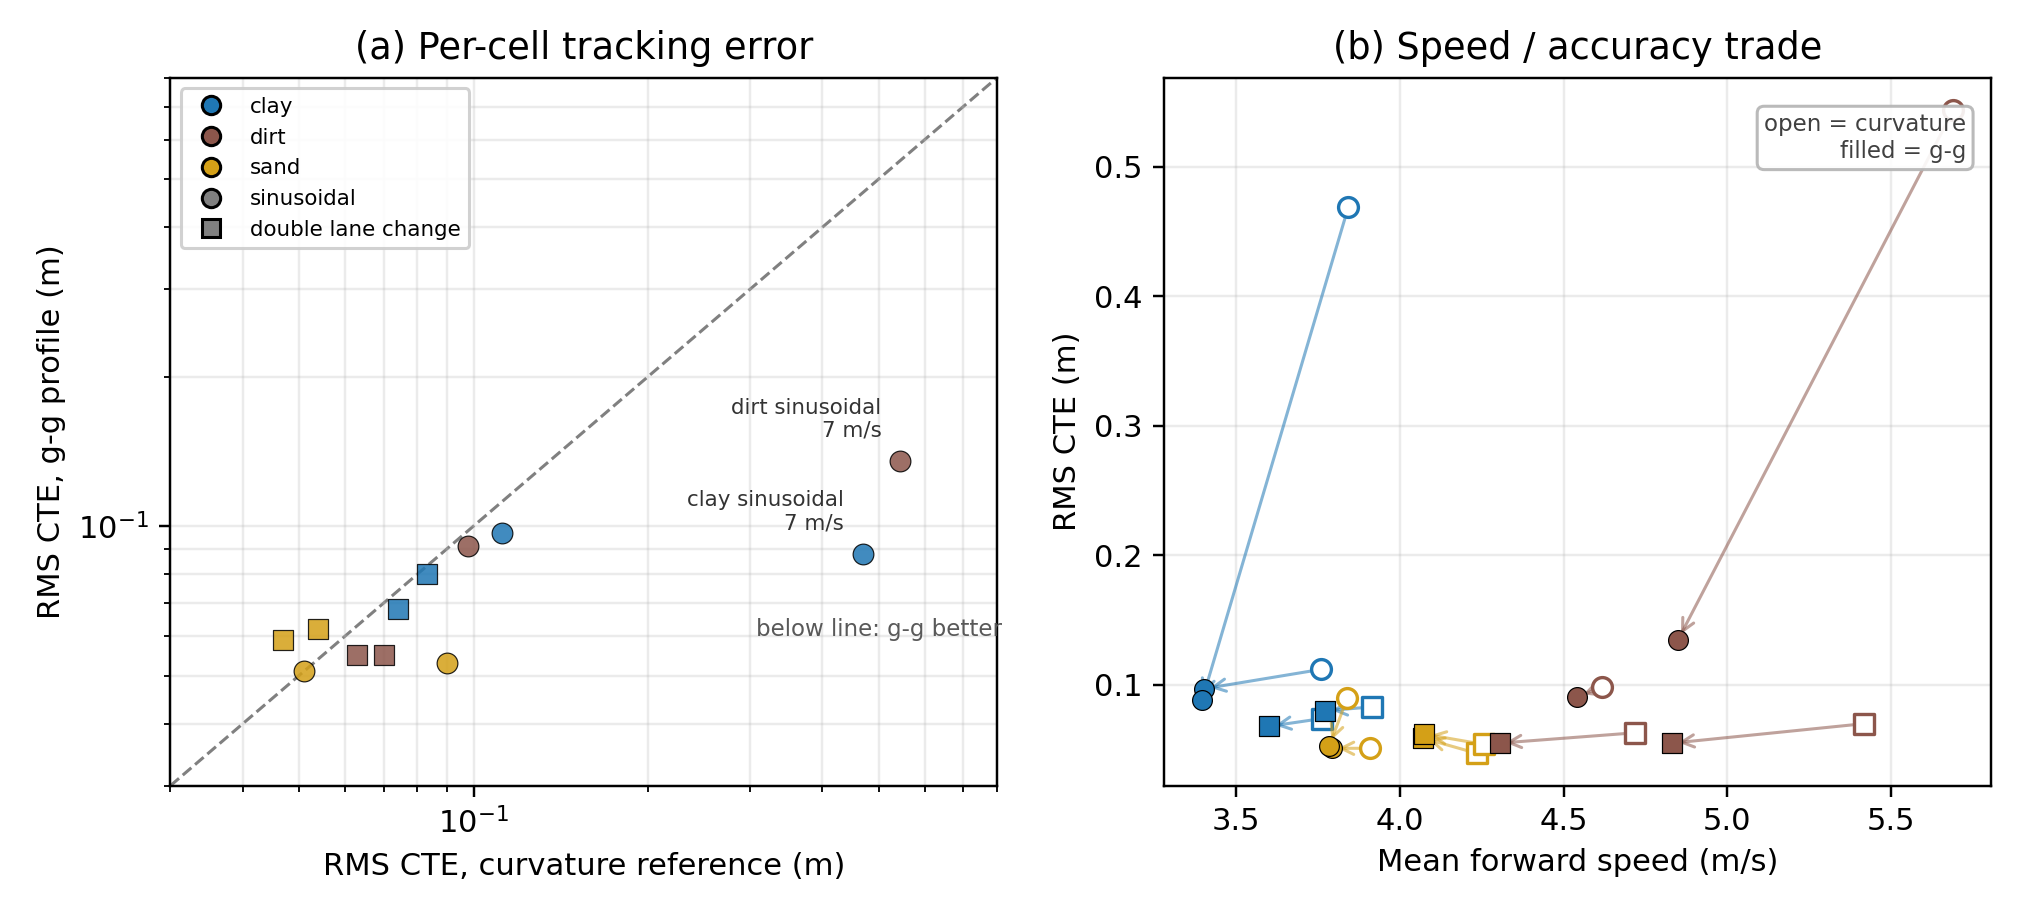
\includegraphics[width=\textwidth]{speed_profile_gg.png}
  \caption{Terrain-aware g--g speed profile vs.\ the geometric
    curvature reference, closed loop. \textbf{(a)} Per-cell RMS CTE: the
    two soft-soil high-speed cells (far right) drop to the trackable
    cluster, while benign cells are unchanged (a few sand cells sit
    marginally above the diagonal, the profile being slightly
    conservative there). \textbf{(b)} Speed/accuracy trade: open markers
    are the curvature reference, filled the g--g profile; arrows show
    each cell trading a little mean speed for a large CTE reduction. The
    grip limits come live from the tyre surrogate at $\hat n$
    (Sec.~\ref{sec:tires}).}
  \label{fig:speedplan}
\end{figure*}

%======================================================================
\section{Asymmetric Throttle Disturbance Observer}
\label{sec:throttledob}
%======================================================================

The bicycle-model NMPC integrates the longitudinal velocity $u$
under the open-loop dynamics $\dot u\!=\!a_x$, with $a_x$ the
commanded longitudinal acceleration. On deformable soil the realised
acceleration is consistently smaller than commanded because of
sinkage drag, producing a steady-state under-speed bias. A
first-order integral disturbance observer on the actuation map
absorbs this bias:
\begin{equation}
  \dot d = \begin{cases}
    K_i (u_{\mathrm{ref}} - u), & u < u_{\mathrm{ref}},\\
    -K_b\, d,                   & u \ge u_{\mathrm{ref}},
  \end{cases}
  \quad |d| \le d_{\max},
\end{equation}
with the bleed gain $K_b\!<\!K_i$ to make the observer asymmetric: it
accumulates rapidly under under-speed and decays slowly toward zero,
never contributing a positive over-speed bias. The applied throttle
is $\tau\!=\!\tau_{\mathrm{NMPC}}\!+\!d$. The ablation zeros both
gains ($K_i\!=\!0$, $d_{\max}\!=\!0$), keeping the structural hook
but suppressing all integral action so the comparison is
apples-to-apples. Table~\ref{tab:throttledob} and
Fig.~\ref{fig:throttledob} report the result over 405 closed-loop
runs per variant.

\begin{table}[!t]
  \renewcommand{\arraystretch}{1.15}
  \caption{Asymmetric throttle disturbance observer ablation.
    405 runs per variant. Speed ratio is reported against the
    \emph{terrain-aware g-g speed profile} (Sec.~\ref{sec:speedplan};
    mean $u_\mathrm{meas}/\mathrm{mean}\,v_\mathrm{ref}(s)$) rather than the
    CLI cruise target, because on curvature-heavy paths the profile
    itself caps below the cruise target -- the cruise target is the
    \emph{intent}, the profile is what the controller is actually
    asked to track. The observer increases achieved speed by approximately
    $5\,\%$ at a negligible ($\sim$3\,mm) increase in tracking error.}
  \label{tab:throttledob}
  \centering
  \setlength{\tabcolsep}{4pt}
  \begin{tabular}{lccc}
    \toprule
    \textbf{Variant} & \textbf{RMS CTE (m)} & \textbf{Speed/profile} & \textbf{$\bar u$ (m/s)}\\
    \midrule
    DOB off & $0.096 \pm 0.044$ & $0.61$ & $4.06$\\
    DOB on  & $0.099 \pm 0.053$ & $\mathbf{0.64}$ & $\mathbf{4.26}$\\
    \bottomrule
  \end{tabular}
\end{table}

\begin{figure*}[!t]
  \centering
  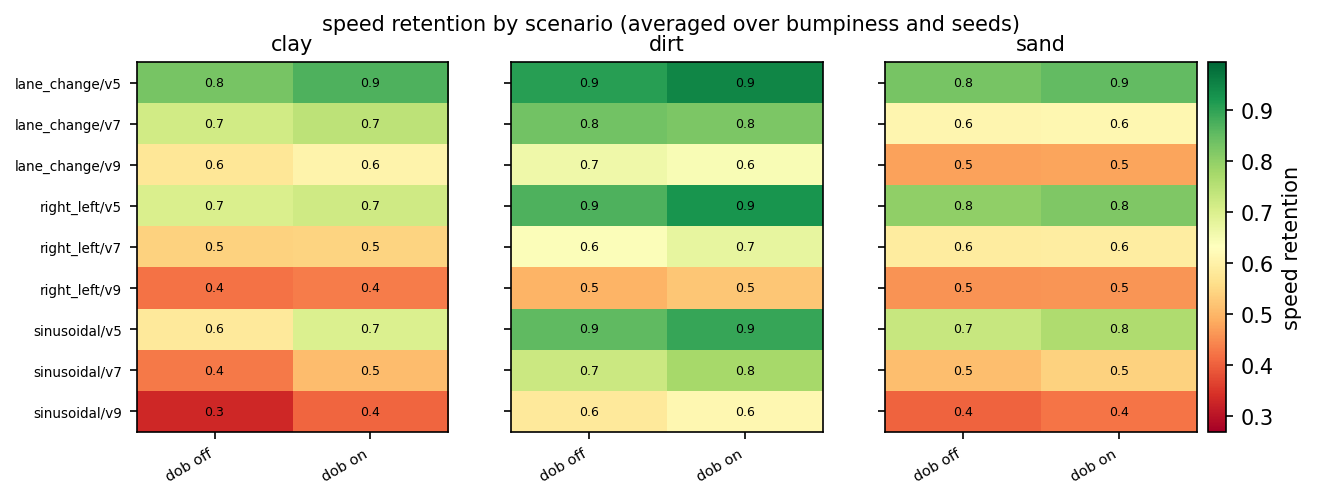
\includegraphics[width=\textwidth]{throttle_dob_ablation_speed_heatmap.png}
  \caption{Throttle disturbance observer ablation: per-scenario
    speed retention (achieved $\bar u$ divided by reference
    $v_{\mathrm{ref}}$) heatmap; row labels show $v_{\mathrm{ref}}$
    and the achieved $\bar u$ so the gap between target and realised
    speed is explicit. The observer's gain is largest on sand at
    $v_{\mathrm{ref}}=7\,\mathrm{m/s}$, consistent with the higher
    sinkage drag in that regime.}
  \label{fig:throttledob}
\end{figure*}

\subsection{Why a reactive observer rather than a feedforward model}
\label{sec:throttledob_ff}
A natural alternative is to make the resistance \emph{feedforward}: the
OCP already exposes a longitudinal residual ($\dot u = a_x +
\mathrm{d}u_\mathrm{resid}$), so one can set
$\mathrm{d}u_\mathrm{resid} = -c_\mathrm{drag}(\hat n)$ with
$c_\mathrm{drag}$ calibrated from the DOB-off rollout drift and indexed
by the live estimate $\hat n$. We implemented and calibrated this, and it
clarifies why the reactive observer is the better choice. First, the
prediction bias is \emph{not} a monotonic drag: only firm soil (dry
sand) genuinely over-predicts speed
($c_\mathrm{drag}\!\approx\!0.17\,\mathrm{m/s^2}$); on dirt the kinematic
prediction \emph{under}-predicts and on clay it is accurate, so the
calibrated feedforward is effectively sand-specific. Second, a
head-to-head over clay/dirt/sand (Table~\ref{tab:ffdrag}) shows the
feedforward term gives only a marginal gain on the calibrated firm
sand (sand speed ratio $0.60\!\to\!0.61$), is inert on clay, and is
mildly adverse on dirt ($0.77\!\to\!0.76$, which under-predicts rather
than over-predicts), but it \emph{cannot replace} the observer: the DOB
is higher on every terrain (clay $0.64$ vs.\ $0.51$, sand $0.65$ vs.\ $0.61$) because
clay's deficit is a traction limit, not a drag, which only integral
feedback closes. Combining the two does not raise speed and inflates
tracking error. A terrain-dependent, sign-varying bias is exactly the
regime where an adaptive observer beats a fixed model, so the DOB is
retained as the default and the feedforward term is left as an optional
firm-soil refinement.

The same conclusion holds for a feedforward at the \emph{actuation map}
itself, the most direct DOB replacement. The naive map
$\tau=a_x/a_{x,\max}$ omits a terrain-dependent throttle offset; the
integral DOB converges to exactly that offset, which is smooth in $\hat
n$ (clay/dirt ${\approx}0.24$, sand ${\approx}0.07$). Baking the
converged offset in as a static held bias $d_\mathrm{ff}(\hat n)$ and
removing the integral (a 48-run clay/dirt/sand ablation) again fails to
replace the observer: it recovers part of the clay deficit
($2.98\!\to\!3.13$ vs.\ DOB $3.41\,$m/s) but \emph{over}-throttles
firmer dirt ($4.55\!\to\!4.43$, below even no compensation) and raises
tracking error, because the required offset is not a static function of
$\hat n$ alone --- it varies with instantaneous speed, curvature, and
load transfer, which the integral tracks online and a terrain-indexed
map cannot. Stacking feedforward and integral matches the DOB's speed
but inflates clay CTE ($0.06\!\to\!0.11\,$m). The longitudinal
disturbance-rejection burden is therefore genuinely adaptive: the DOB is
not a tunable patch over a poor model but a necessary closed-loop
element.

\begin{table}[!t]
  \renewcommand{\arraystretch}{1.15}
  \caption{Feedforward sinkage-drag vs.\ the reactive DOB --- mean speed
    ratio (achieved $\bar u$ / reference), sinusoidal path,
    $v\!\in\!\{5,7\}\,$m/s, two seeds. \emph{off}: neither;
    \emph{ffdrag}: feedforward drag, DOB off; \emph{DOB}: reactive
    observer. The feedforward term helps where calibrated (sand, dirt)
    but trails the DOB on every terrain.}
  \label{tab:ffdrag}
  \centering
  \setlength{\tabcolsep}{6pt}
  \begin{tabular}{lccc}
    \toprule
    \textbf{Terrain} & \textbf{off} & \textbf{ffdrag} & \textbf{DOB}\\
    \midrule
    clay & $0.50$ & $0.51$ & $\mathbf{0.64}$\\
    dirt & $0.77$ & $0.76$ & $\mathbf{0.80}$\\
    sand & $0.60$ & $0.61$ & $\mathbf{0.65}$\\
    \bottomrule
  \end{tabular}
\end{table}

%======================================================================
\section{Two-Layer Obstacle Avoidance}
\label{sec:safety}
%======================================================================

The planner adds a smooth softplus barrier to the stage and terminal
costs for each known obstacle. Downstream of the planner and human
command source, the \texttt{SAFETY\_FILTERS} registry exposes a
common \texttt{filter} interface: the filter receives the desired
steering, throttle, brake, the current state, and the nearby
obstacles, and returns the filtered command plus diagnostics. The
DOB-CBF variant solves a single-step minimum-deviation QP around the
incoming command --- the natural intent-preserving mechanism for HIL
teleoperation --- and logs intervention rate and command deviation as
an intrusiveness signal. The MPPI variant runs at the controller rate,
samples $K\!=\!384$ noisy command sequences, rolls each forward
through the same neural tire surrogate the planner uses over a
horizon padded by the exponentially smoothed round-trip delay, and
returns the importance-weighted mean of the first action. Its cost
combines (i)~a softplus obstacle barrier inflated by a
stopping-distance buffer, (ii)~a neural-surrogate-derived
friction-cone penalty, (iii)~a terrain-aware speed cap, and
(iv)~deviation from operator intent.

\paragraph{Seed trajectories.}
The sample set is augmented with six hand-crafted seed sequences
(passthrough, full brake, coast straight, evade-left,
evade-right, brake-while-turn) injected unconditionally. The
intent is to guarantee that at least one safe option is present in
the sample set even when every Gaussian-perturbed sample around the
operator command is unsafe. Section~\ref{sec:safety_seeds} reports
an ablation that confirms the seeds are not optional.

\paragraph{Comparison filters.}
The safety-filter contract is evaluated with (i) the DOB-CBF filter of
Zhang et al.~\cite{Zhang25}, optionally evaluated on the same neural
surrogate; (ii) the MPPI predictive safety filter; (iii) a gradient-based
NMPC variant solved via SLSQP on the identical rollout; and (iv) no
filter.

\subsection{Human-in-the-loop safety-filter protocol}
\label{sec:safety_hil}

The safety filter exists to screen a \emph{human operator's}
delayed commands; the framework therefore includes a human-in-the-loop
(HIL) protocol in addition to the autonomous sweeps reported below. A
human drives the HMMWV through the rock field from the Chrono::Sensor
driver point-of-view using a Logitech G29 steering wheel, while the
sim-side filter screens the operator commands immediately before
vehicle actuation. Each round delays \emph{both} teleoperation
channels: the operator command path (uplink) by
$\Delta_\mathrm{cmd} \in \{0, 0.15, 0.30\}\,\mathrm{s}$ and the
driver-camera feed (downlink) by
$\Delta_\mathrm{cam} = s\,\Delta_\mathrm{cmd}$, where the camera-delay
scale $s$ defaults to $1.0$ for a symmetric link. The same script
supports a profile-driven delay for learned 5G traces.

The HIL comparison repeats each (filter, delay) cell over multiple
driver rounds and logs both safety and intrusiveness metrics:
collisions, minimum clearance, intervention rate, mean steering
correction, mean throttle/brake correction, and speed retention. The
intervention metrics matter because the safety filter should preserve
operator intent whenever the human command is already safe. The
human-in-the-loop layer reuses the same command contract, swappable
safety filters, and metric pipeline as the autonomous evaluation.
Table~\ref{tab:hil} and Figs.~\ref{fig:hil_summary}--\ref{fig:hil_heatmap}
report the human-driven rounds; the autonomous protocol of the following
section complements them with a large, fully repeatable multi-seed matrix
that removes inter-operator variance.

\paragraph{Human-in-the-loop results.}
\emph{[Placeholder --- to be completed after the HIL rounds are run; sims
pending.]} Across the four filters and the
$\Delta_\mathrm{cmd}\!\in\!\{0,0.15,0.30\}\,$s operator-latency sweep we
report, per driver round, collisions, minimum clearance, intervention rate,
mean steering and throttle correction, and speed retention. The expected
reading is that the DOB-CBF and MPPI filters cut collisions relative to the
no-filter baseline while holding a low intervention rate and small command
deviation (operator intent is preserved whenever the human command is
already safe), corroborating the autonomous safety-filter-only sweep of
Sec.~\ref{sec:safety_blind}.

\begin{table}[!t]
  \renewcommand{\arraystretch}{1.10}
  \caption{\textbf{[PLACEHOLDER --- pending HIL runs.]} Human-in-the-loop
    safety-filter comparison (Logitech G29 operator, rock field) at
    operator delay $\Delta_\mathrm{cmd}=0.15\,$s, averaged over driver
    rounds; the full $\{0,0.15,0.30\}\,$s latency sweep and the per-tick
    steering/throttle intrusiveness are in Fig.~\ref{fig:hil_summary}.
    Values pending the HIL sim runs.}
  \label{tab:hil}
  \centering
  \begin{tabular}{lcccc}
    \toprule
    \textbf{Filter} & Coll./run & Clearance (m) & Interv.\ (\%)
        & Speed ret.\\
    \midrule
    None     & -- & -- & -- & --\\
    DOB-CBF  & -- & -- & -- & --\\
    MPPI     & -- & -- & -- & --\\
    NMPC     & -- & -- & -- & --\\
    \bottomrule
  \end{tabular}
\end{table}

\begin{figure*}[!t]
  \centering
  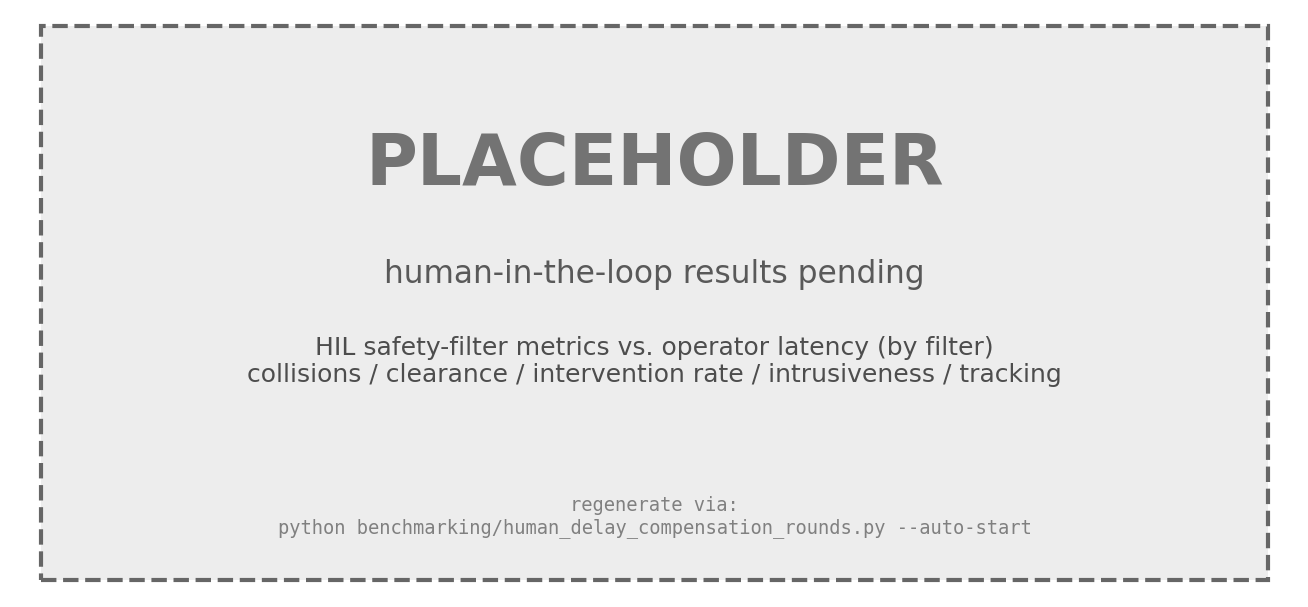
\includegraphics[width=\textwidth]{human_delay_compensation_summary.png}
  \caption{\textbf{[PLACEHOLDER --- pending HIL runs.]} Human-in-the-loop
    safety-filter metrics versus operator/link latency
    $\Delta_\mathrm{cmd}\!\in\!\{0,0.15,0.30\}\,$s, one curve per filter
    (none / DOB-CBF / MPPI / NMPC): collisions, minimum clearance,
    intervention rate, mean throttle/steering correction, and RMS CTE. To
    be generated from the HIL rounds
    (\texttt{human\_delay\_compensation\_rounds.py}).}
  \label{fig:hil_summary}
\end{figure*}

\begin{figure}[!t]
  \centering
  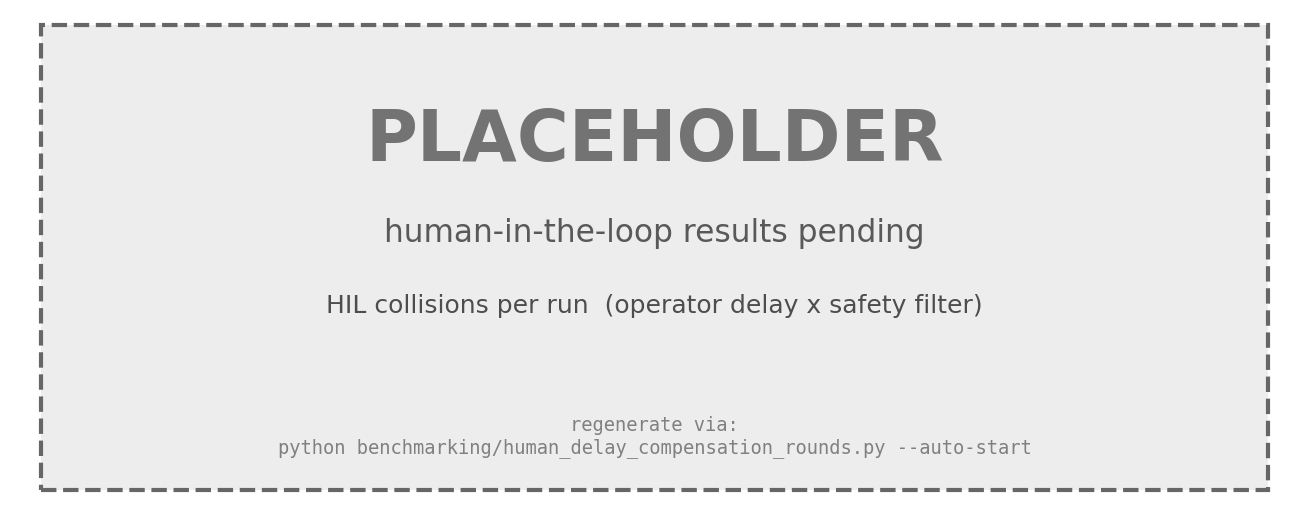
\includegraphics[width=\columnwidth]{human_delay_collision_heatmap.png}
  \caption{\textbf{[PLACEHOLDER --- pending HIL runs.]} Human-in-the-loop
    collisions per run across operator delay $\times$ safety filter. To be
    generated from the HIL rounds.}
  \label{fig:hil_heatmap}
\end{figure}


\subsection{Autonomous validation: safety-filter-only collision avoidance}
\label{sec:safety_blind}

The HIL protocol of Section~\ref{sec:safety_hil} is complemented by
an autonomous controlled experiment in which an obstacle-blind planner
stands in for the operator, isolating the safety filter as the sole collision
avoider. This
removes operator variance and supports a larger, fully repeatable
matrix (405 trials per filter; 1620 trials total). The same matrix is
re-evaluated with the planner's in-horizon barriers re-enabled in
Sec.~\ref{sec:safety_aware} for a total of 3240 runs.
Table~\ref{tab:safety_blind} and Fig.~\ref{fig:safety_blind} report the
safety-filter-only outcome. Because the planner's reference here is
deliberately routed through the obstacles, the crosstrack-error (CTE)
column does not measure tracking quality: it measures how far an active
safety filter must pull the vehicle off that obstacle-blind reference to stay
safe, and therefore reads as an intrusiveness proxy. A larger CTE for
DOB-CBF and NMPC than for MPPI is consistent with their higher
per-step deviation, not with worse tracking.

\begin{table}[!t]
  \renewcommand{\arraystretch}{1.10}
  \caption{Autonomous safety-filter-only validation (planner blind to
    obstacles). 405 runs per filter (1620 total); same scenario matrix
    as Table~\ref{tab:safety_aware}, blind rows only. MPPI achieves the
    lowest mean collisions \emph{and} the largest clearance margin;
    DOB-CBF is the least intrusive safety filter (lowest intervention rate),
    the natural intent-preserving filter for the HIL case in
    Sec.~\ref{sec:safety_hil}.}
  \label{tab:safety_blind}
  \centering
  \setlength{\tabcolsep}{4pt}
  \begin{tabular}{lcccc}
    \toprule
    \textbf{Filter} & \textbf{Coll./run} & \textbf{Clearance (m)} & \textbf{Interv. (\%)} & \textbf{CTE (m)}\\
    \midrule
    None         & $3.05$ & $-1.83$ & --- & $0.25$\\
    \textbf{DOB-CBF} & $0.46$ & $+0.26$ & $\mathbf{52}$ & $2.29$\\
    \textbf{MPPI}    & $\mathbf{0.10}$ & $\mathbf{+2.17}$ & $88$ & $1.13$\\
    NMPC (SLSQP) & $0.45$ & $+1.13$ & $84$ & $7.26$\\
    \bottomrule
  \end{tabular}
\end{table}

\begin{figure*}[!t]
  \centering
  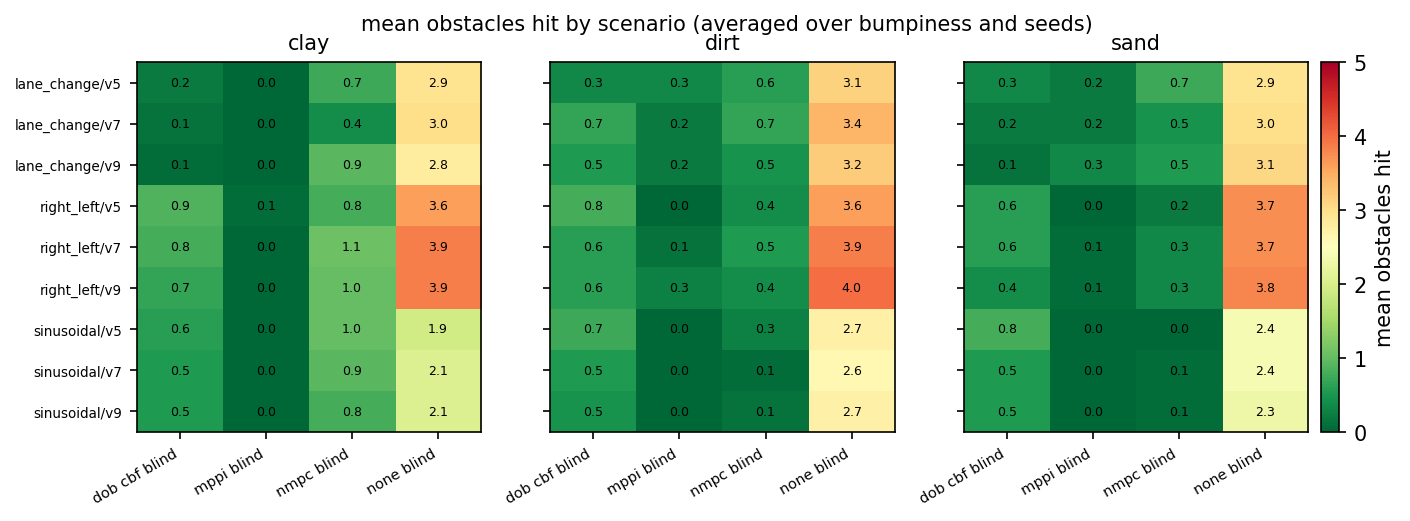
\includegraphics[width=\textwidth]{safety_filter_collision_heatmap.png}
  \caption{Autonomous safety-filter-only validation. Mean unique obstacles hit
    per run, stratified by terrain and safety filter, with whisker
    error bars showing across-seed standard deviation. The reported
    sweep covers all three deployment terrains (clay, dirt, sand) across
    three speeds and three bumpiness levels, $135$ runs per (filter,
    terrain) cell. Aggregate KPIs are in
    Table~\ref{tab:safety_blind}.}
  \label{fig:safety_blind}
\end{figure*}

\subsection{Two-layer (planner-aware) stack}
\label{sec:safety_aware}

With the in-horizon NMPC barrier re-enabled the two-layer stack is
evaluated. Table~\ref{tab:safety_aware} reports 3240 runs total
across all four safety-filter variants under both planner-aware and
planner-blind modes.
Barriers alone (no-filter, planner-aware) cut collisions by approximately
$6\times$ relative to the planner-blind baseline ($3.01\to0.49$ per
run), and combining the barrier with the DOB-CBF or MPPI filter drives
collisions to near zero ($0.20$ and $0.04$ per run, respectively).

\begin{table}[!t]
  \renewcommand{\arraystretch}{1.10}
  \caption{Planner-aware vs.\ planner-blind safety sweep. 3240 runs.
    The two-layer stack (barrier $+$ safety filter) drives collisions to near
    zero ($\le 0.20$/run) for both DOB-CBF and MPPI filters.}
  \label{tab:safety_aware}
  \centering
  \setlength{\tabcolsep}{4pt}
  \begin{tabular}{lcccc}
    \toprule
    \textbf{Variant} & \textbf{Coll./run} & \textbf{Clearance (m)} & \textbf{Interv. (\%)} & \textbf{CTE (m)}\\
    \midrule
    None, blind          & $3.01$ & $-1.83$ & --- & $0.25$\\
    None, aware          & $0.49$ & $+0.39$ & --- & $2.44$\\
    DOB-CBF, blind       & $0.50$ & $+0.22$ & $52$ & $2.43$\\
    \textbf{DOB-CBF, aware} & $\mathbf{0.20}$ & $+1.24$ & $35$ & $2.74$\\
    MPPI, blind          & $0.07$ & $+2.23$ & $88$ & $1.24$\\
    \textbf{MPPI, aware}    & $\mathbf{0.04}$ & $+2.07$ & $84$ & $2.69$\\
    NMPC, blind          & $0.51$ & $+1.11$ & $84$ & $6.95$\\
    NMPC, aware          & $0.26$ & $+1.35$ & $80$ & $7.58$\\
    \bottomrule
  \end{tabular}
\end{table}


\subsection{DOB-CBF neural-surrogate ablation}
\label{sec:safety_dobcbf}

The DOB-CBF filter can run either with the neural tire surrogate
enabled or with a kinematic/linear fallback. In the fallback mode the
disturbance observer uses fixed longitudinal acceleration limits, the
CBF uses kinematic steering authority, and the terrain speed cap omits
the NN traction check. With the NN enabled, the same QP receives
terrain-aware longitudinal acceleration, lateral-force, yaw-moment,
and traction-limit estimates from the whole-vehicle surrogate.
Table~\ref{tab:dobcbf_nn} and Fig.~\ref{fig:dobcbf_nn} compare the
two variants over 1215 closed-loop trials.

\begin{table}[!t]
  \renewcommand{\arraystretch}{1.10}
  \caption{DOB-CBF neural-surrogate ablation. 1215 runs.}
  \label{tab:dobcbf_nn}
  \centering
  \setlength{\tabcolsep}{3pt}
  \begin{tabular}{lcccc}
    \toprule
    \textbf{Variant} & \textbf{Coll./run} & \textbf{Clearance (m)} & \textbf{Interv. (\%)} & \textbf{CTE (m)}\\
    \midrule
    No filter        & $3.05$ & $-1.83$ & --- & $0.27$\\
    DOB-CBF, no NN   & $0.81$ & $-0.21$ & $46$ & $1.92$\\
    \textbf{DOB-CBF, with NN} & $\mathbf{0.48}$ & $\mathbf{+0.12}$ & $50$ & $2.20$\\
    \bottomrule
  \end{tabular}
\end{table}

\begin{figure*}[!t]
  \centering
  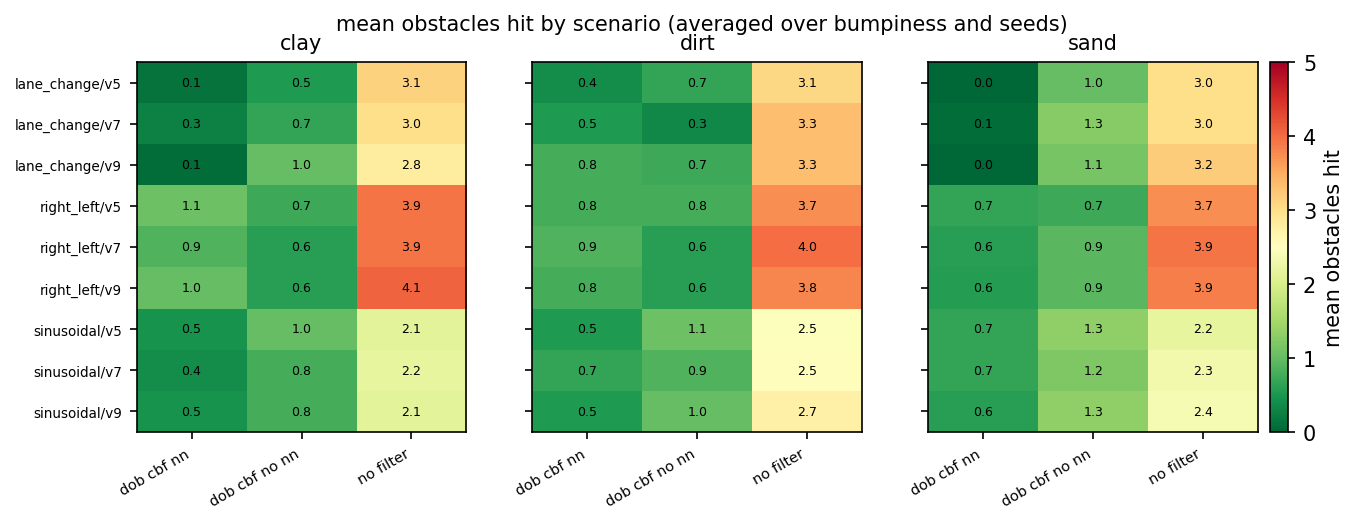
\includegraphics[width=\textwidth]{dob_cbf_nn_ablation_heatmap.png}
  \caption{DOB-CBF neural-surrogate ablation: per-scenario
    collisions. Aggregate KPIs are in Table~\ref{tab:dobcbf_nn}.}
  \label{fig:dobcbf_nn}
\end{figure*}

\subsection{MPPI seed-trajectory ablation}
\label{sec:safety_seeds}

The contribution of the hand-crafted seed trajectories is
quantified by disabling the seed-injection logic and forcing the
safety filter to rely solely on Gaussian sampling around the operator
command. Table~\ref{tab:mppi_seeds} and Fig.~\ref{fig:mppi_seeds}
report the result over 810 closed-loop trials. Removing the seeds
increases the collision rate by approximately 27$\times$ and drives
the minimum clearance into the obstacle footprint.

\begin{table}[!t]
  \renewcommand{\arraystretch}{1.10}
  \caption{MPPI seed-trajectory ablation. 810 runs.}
  \label{tab:mppi_seeds}
  \centering
  \setlength{\tabcolsep}{4pt}
  \begin{tabular}{lcccc}
    \toprule
    \textbf{Variant} & \textbf{Coll./run} & \textbf{Clearance (m)} & \textbf{Interv. (\%)} & \textbf{CTE (m)}\\
    \midrule
    MPPI, no seeds   & $2.18$ & $-1.05$ & $86$ & $0.98$\\
    \textbf{MPPI, with seeds} & $\mathbf{0.08}$ & $\mathbf{+2.03}$ & $88$ & $1.03$\\
    \bottomrule
  \end{tabular}
\end{table}

\begin{figure*}[!t]
  \centering
  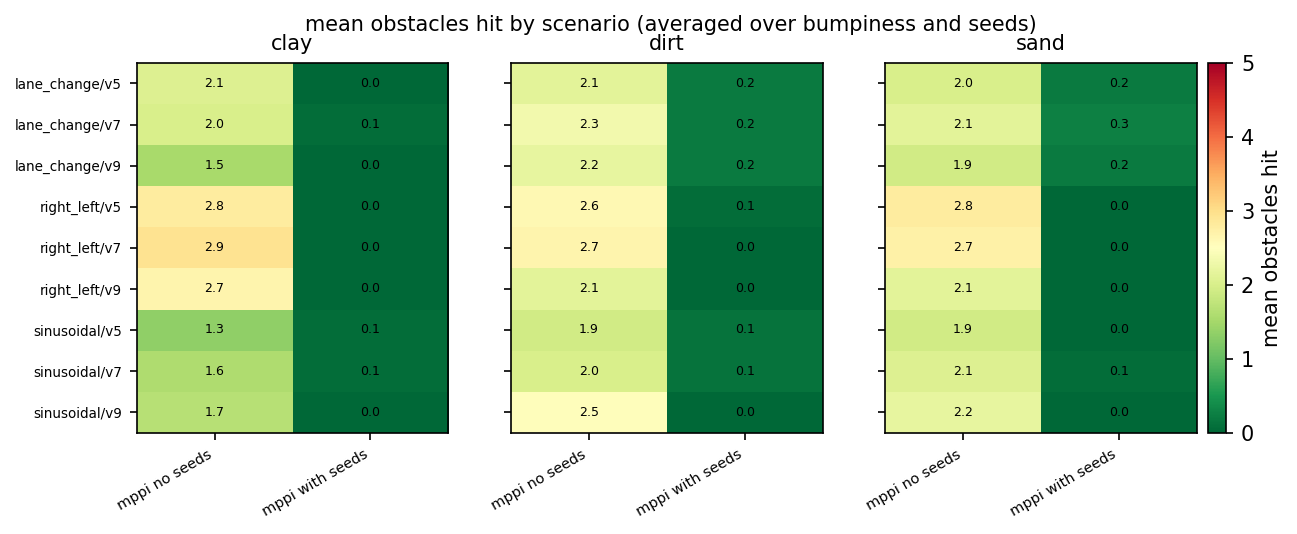
\includegraphics[width=\textwidth]{mppi_seed_ablation_collision_heatmap.png}
  \caption{MPPI seed-trajectory ablation. Removing the seeds
    eliminates the safety filter's commitment to evasive maneuvers; the
    weighted mean then averages over many comparably high-error samples
    rather than concentrating on a recoverable trajectory.}
  \label{fig:mppi_seeds}
\end{figure*}

\subsection{Planner tire model under a fixed MPPI filter}
\label{sec:safety_tire}

A separate sweep runs the autonomous obstacle scenario with the
MPPI filter always on, varying only the planner's tire model (the
analytical planners use the SCM-calibrated parameters of
Sec.~\ref{sec:tires_static}). All three tire models avoid the obstacles
approximately equally
(Table~\ref{tab:auto_obstacle} and Fig.~\ref{fig:auto_obstacle}),
indicating that the safety filter dominates the filter-mediated outcome
and that the planner-tire choice is largely orthogonal to the
safety outcome.

\begin{table}[!t]
  \renewcommand{\arraystretch}{1.10}
  \caption{Autonomous obstacle avoidance, planner tire model swept
    under a fixed MPPI filter (analytical planners SCM-calibrated).
    1215 runs (405 per model).}
  \label{tab:auto_obstacle}
  \centering
  \begin{tabular}{lccc}
    \toprule
    \textbf{Planner tire model} & \textbf{Coll./run} &
    \textbf{Clearance (m)} & \textbf{CTE (m)}\\
    \midrule
    Pacejka              & $0.01$ & $+3.05$ & $0.49$\\
    TMeasy               & $0.01$ & $+2.92$ & $0.49$\\
    NN rate-MLP          & $0.03$ & $+3.14$ & $0.56$\\
    \bottomrule
  \end{tabular}
\end{table}

\begin{figure*}[!t]
  \centering
  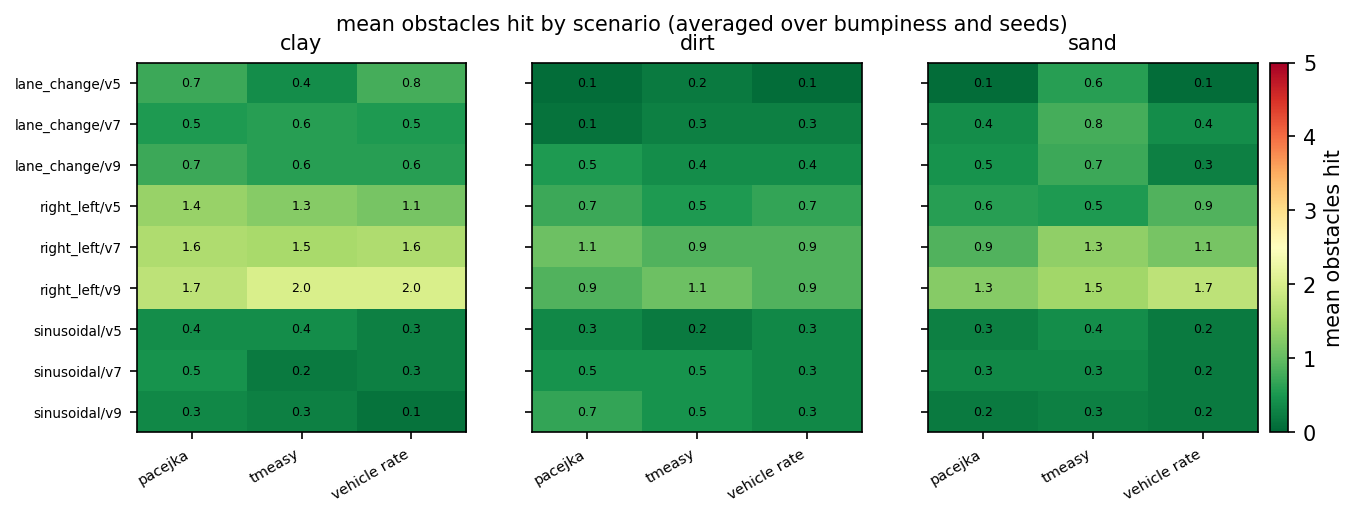
\includegraphics[width=\textwidth]{autonomous_obstacle_collision_heatmap.png}
  \caption{Autonomous obstacle avoidance, planner tire model swept
    under a fixed MPPI filter. Mean unique obstacles hit per run
    stratified by terrain with across-seed whisker error bars; the
    three tire models are statistically indistinguishable here because
    the safety filter, not the planner-tire choice, dominates the safety
    outcome. Sweep matrix is clay/dirt/sand $\times$ 3 paths $\times$ 3
    speeds $\times$ 3 bumpiness $\times$ 5 seeds.
    Aggregate KPIs are in Table~\ref{tab:auto_obstacle}.}
  \label{fig:auto_obstacle}
\end{figure*}

%======================================================================
\section{5G-Profile Latency Robustness}
\label{sec:latency}
%======================================================================

A sequence model (N-HiTS) is trained on the public 5G YouTube
uplink dataset of Choi et al.~\cite{Choi23} and used to generate a
synthetic bitrate trace. The trace is mapped through a configurable
queue-load model to produce a per-channel latency profile that is
applied as an additive scheduled delay on the camera and command
channels.

\begin{figure}[!t]
  \centering
  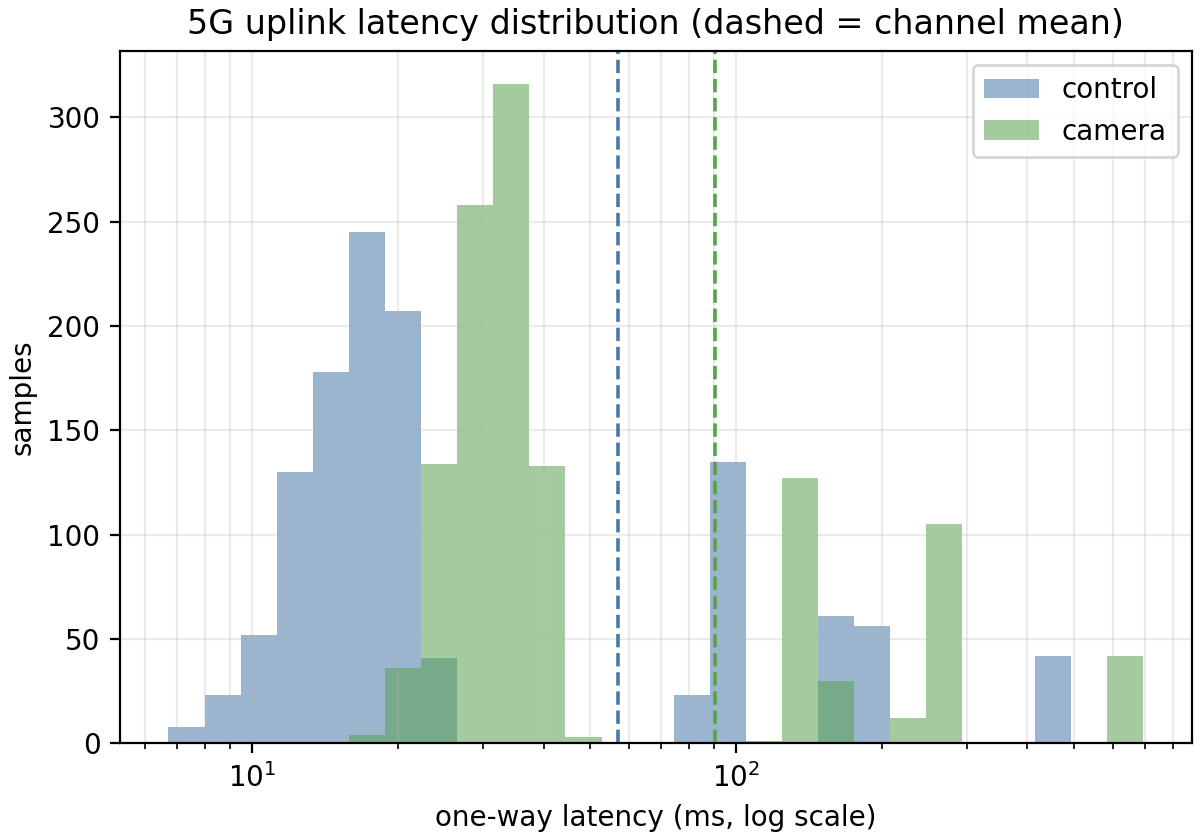
\includegraphics[width=\columnwidth]{latency_profile_histogram.png}
  \caption{Learned N-HiTS 5G uplink profile applied to the camera and
    control channels (log-$x$ histogram; dashed lines are channel
    means). The profile is bimodal: a low-latency good-window bulk
    (control around $10$--$25\,\mathrm{ms}$, camera around
    $30$--$50\,\mathrm{ms}$), a poor-window cluster near
    $100$--$200\,\mathrm{ms}$, and discrete outage spikes at
    $450\,\mathrm{ms}$ (control) and $660\,\mathrm{ms}$ (camera). Mean
    one-way latency is approximately $94\,\mathrm{ms}$ (control) and
    $144\,\mathrm{ms}$ (camera).}
  \label{fig:latency_profile}
\end{figure}

The closed-loop obstacle scenario is then run under the synthetic
profile with three filter configurations:
Table~\ref{tab:latency_comp} and Fig.~\ref{fig:latency_comp}
report the result over 1215 trials. Both safety filter variants reduce
collisions by more than 90\,\% relative to the no-filter
baseline (DOB-CBF by $99.6\,\%$, MPPI by $96\,\%$).

\begin{table}[!t]
  \renewcommand{\arraystretch}{1.10}
  \caption{Closed-loop collisions under the learned N-HiTS-5G
    latency profile. 1215 runs.}
  \label{tab:latency_comp}
  \centering
  \begin{tabular}{lccc}
    \toprule
    \textbf{Filter} & \textbf{Coll./run} & \textbf{Clearance (m)} & \textbf{Interv. (\%)}\\
    \midrule
    None      & $2.47$ & $-1.42$ & ---\\
    DOB-CBF   & $\mathbf{0.01}$ & $+2.53$ & $54$\\
    MPPI      & $0.10$ & $\mathbf{+3.28}$ & $86$\\
    \bottomrule
  \end{tabular}
\end{table}

\begin{figure*}[!t]
  \centering
  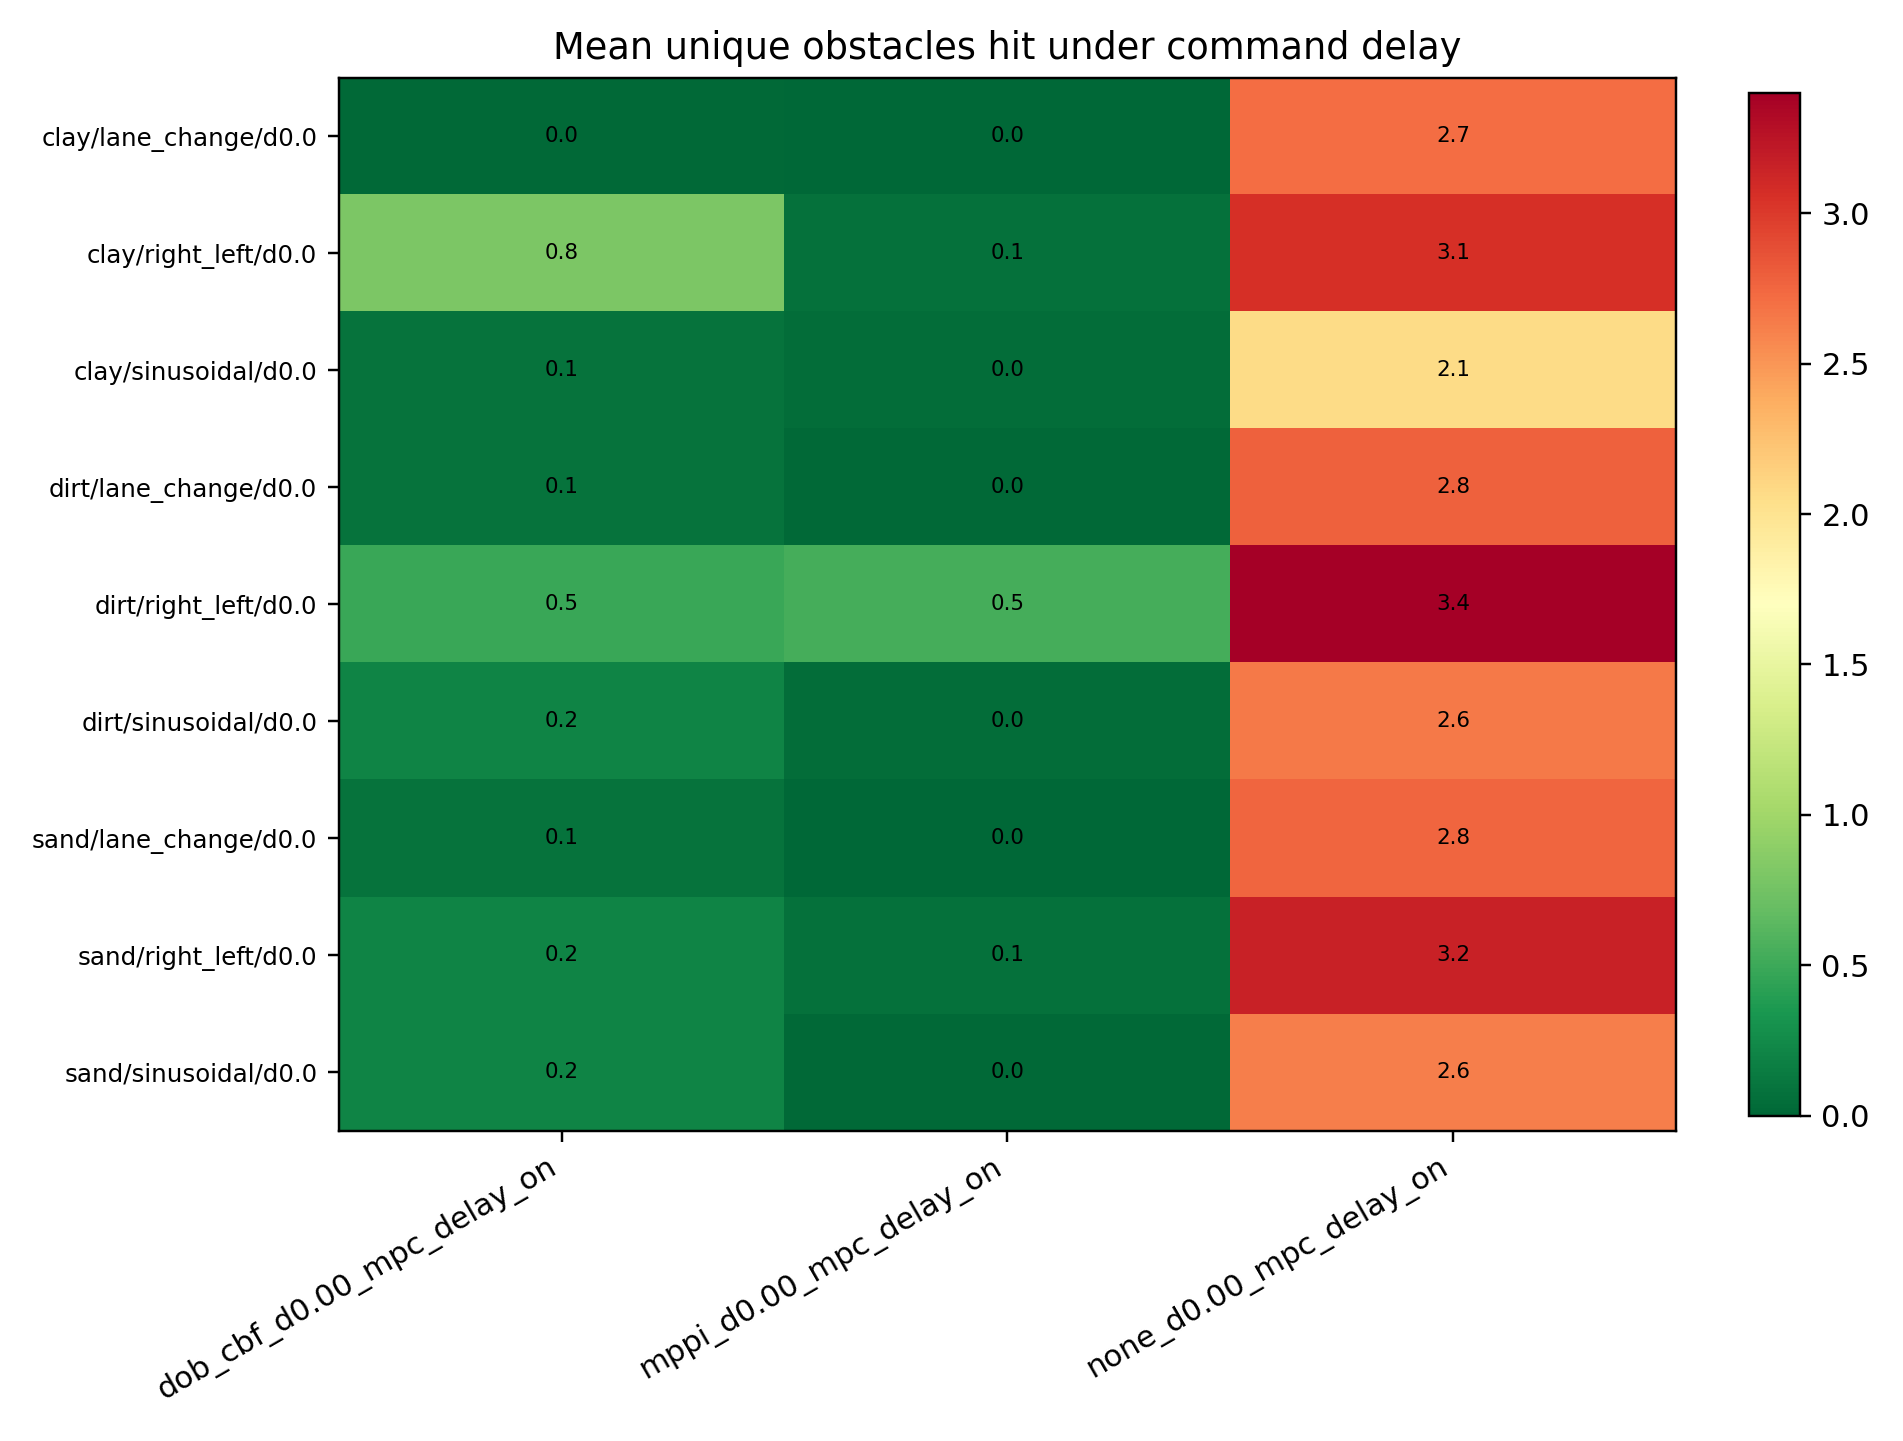
\includegraphics[width=\textwidth]{latency_compensation_collision_heatmap.png}
  \caption{5G-profile latency compensation sweep: per-scenario
    collisions. Aggregate KPIs are in Table~\ref{tab:latency_comp}.}
  \label{fig:latency_comp}
\end{figure*}

%======================================================================
\section{Terrain- and Latency-Aware Collision Warning}
\label{sec:collision_warning}
%======================================================================

The safety filters in
\S\ref{sec:safety}--\S\ref{sec:latency} modify the
operator's command stream when a collision is imminent. In some
deployment modes (e.g. expert-loop teleoperation, or a safety filter
that has been muted for debugging) the operator wants only a
\emph{notification} rather than a control override. We add an
independent forward collision warning component that runs in parallel
with the rest of the stack and emits a discrete severity signal
$\{\textsc{green}, \textsc{yellow}, \textsc{orange}, \textsc{red}\}$
on every controller tick.

The warning module is exposed through a small factory in line with
the rest of the swappable safety layer, so the warning strategy can
be selected at construction time. The default strategy is a
time-to-collision predictor with two adjustments:

\paragraph{Terrain awareness.} The required stopping distance
$d_{\mathrm{stop}}=v\tau_{r}+v^{2}/(2a_{b})$ uses a brake-deceleration
$a_{b}(\hat n)$ that is computed \emph{analytically at init time} by
querying the same rig tire surrogate the
DOB-CBF and MPC use for traction-budget queries. For every $\hat n
\in [0.40,1.30]$ on a 0.05 grid, the surrogate is loaded with the
manifold-interpolated Bekker vector at that $\hat n$, swept over
braking slip ratios $\kappa\in[-0.40,0]$ at static per-wheel $F_z$,
and the peak $|F_x|$ at front and rear axles is summed to give the
total available braking force; $a_b(\hat n)=\sum F_{x,\mathrm{peak}}
/ m_{\mathrm{veh}}$. The resulting table runs from
$a_b(0.4)\!\approx\!2.3\,\mathrm{m/s^{2}}$ (soft, clay-like) to
$a_b(1.1)\!\approx\!4.7\,\mathrm{m/s^{2}}$ (firm, sand-like) — both
endpoints noticeably more conservative than the hand-tuned
$2.5/6.0\,\mathrm{m/s^{2}}$ heuristic the implementation previously
used. The live $\hat n$ from the online terrain estimator
(\S\ref{sec:estimator}) indexes into this table at runtime, so the
warning is more conservative on soils that the vehicle cannot brake
hard on.

\paragraph{Brake-decel validation.}
The analytical $a_b(\hat n)$ table is validated against actual Chrono
SCM behaviour with 27 full-brake stops: three terrains $\times$
three initial speeds $\{3,5,7\}\,\mathrm{m/s}$ $\times$ three seeds,
each scenario cruising to target speed and then applying
$\mathrm{brake}=1$, $\mathrm{throttle}=0$ until the vehicle is below
$0.2\,\mathrm{m/s}$. Stopping distance and mean decel are extracted
from the recorded chassis trajectory and compared to the prediction
at the brake-onset speed (Fig.~\ref{fig:cw_brake_validation}). On
mean decel, the rig-NN analytical table is within $0.1\,\mathrm{m/s^{2}}$
on clay, over-predicts dirt by $0.7\,\mathrm{m/s^{2}}$ (the
classical contact-patch saturation gap of \S\ref{sec:tires_rig_vs_vehicle}),
and over-predicts sand by $1.1\,\mathrm{m/s^{2}}$ — small enough
that the resulting stopping-distance prediction lands within
$\pm 0.5\,\mathrm{m}$ of the recorded ground truth on 23 of 27
trials. Aggregated mean $|\Delta d_{\mathrm{stop}}|$ is
$0.17\,\mathrm{m}$ for the analytical table versus $0.45\,\mathrm{m}$
for the hand-tuned linear-interp fallback ($2.6\times$ improvement);
the analytical prediction also has a small positive mean bias
($+0.10\,\mathrm{m}$), meaning the warning is biased toward firing
slightly earlier than strictly necessary, which is the safe
direction.

\begin{figure*}[!t]
  \centering
  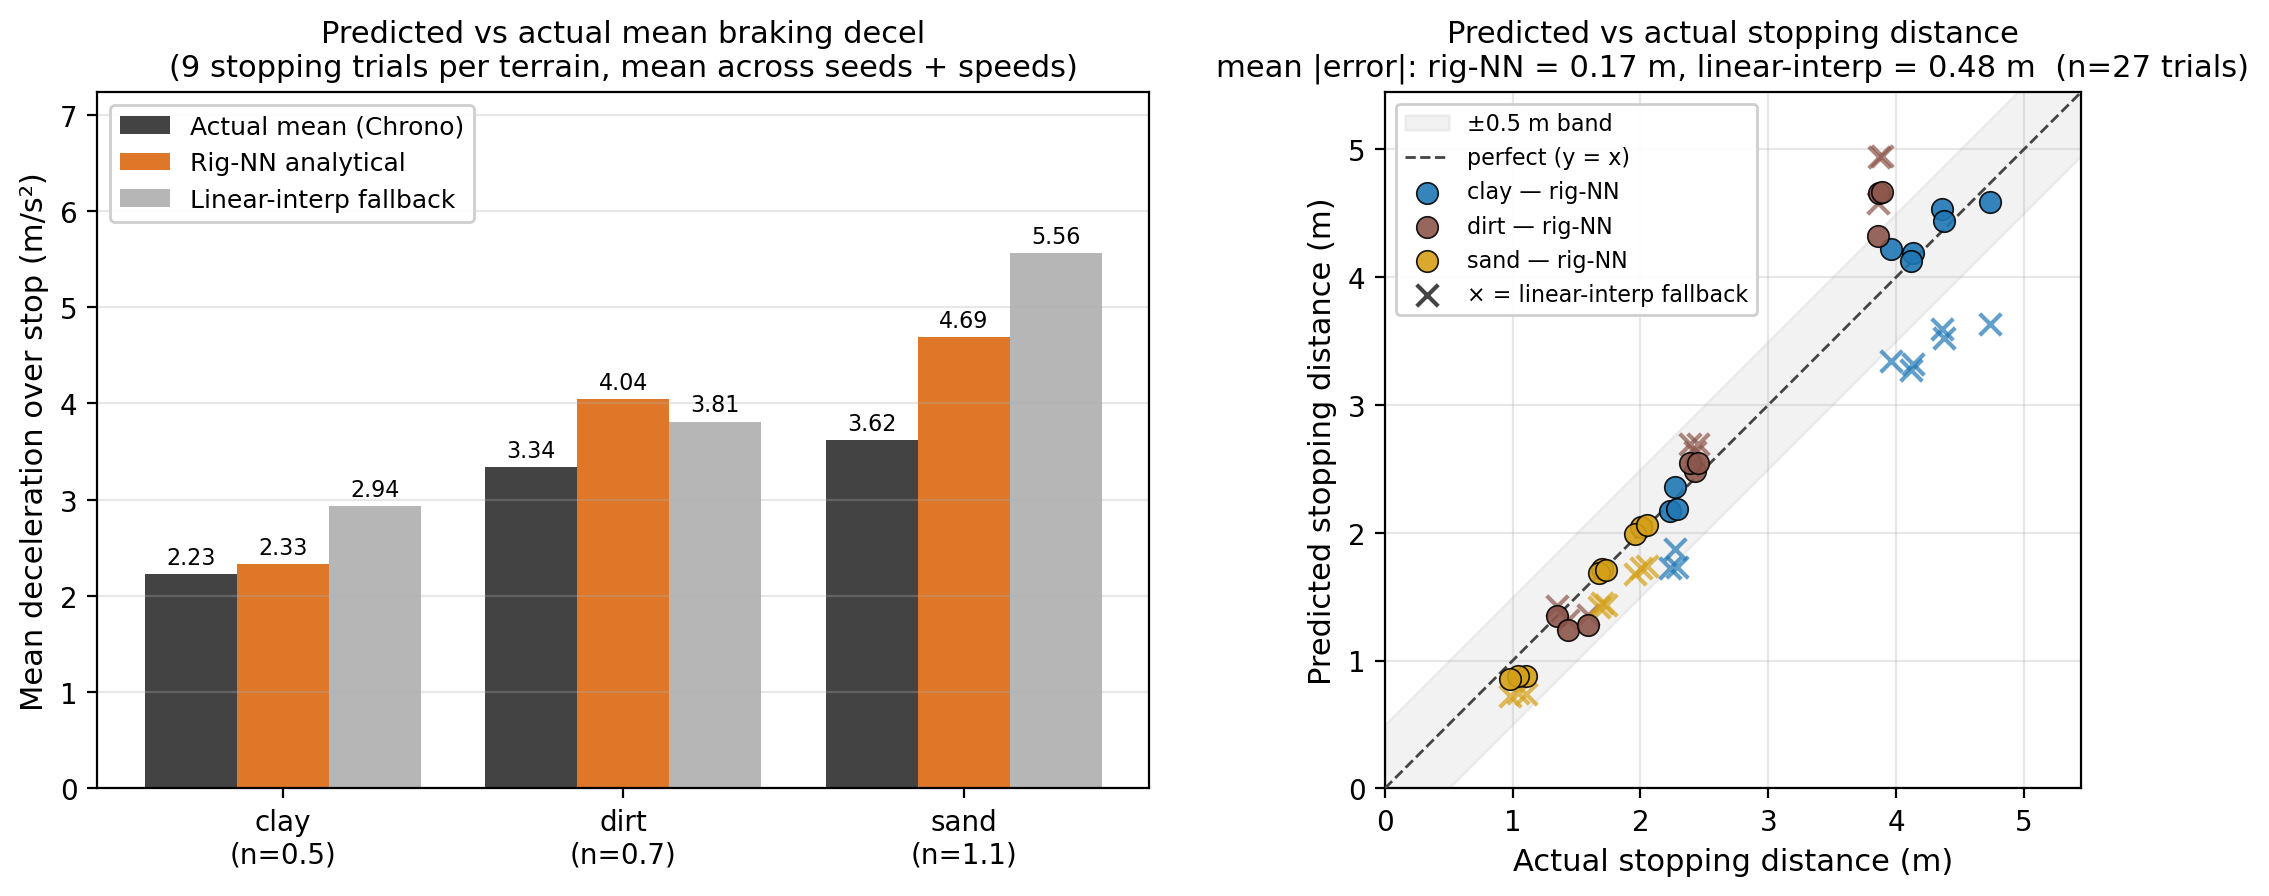
\includegraphics[width=\textwidth]{cw_brake_validation.png}
  \caption{Validation of the warning system's analytical
    brake-deceleration table against actual Chrono SCM stopping
    behaviour (27 trials, 3 terrains $\times$ 3 initial speeds
    $\times$ 3 seeds). Left: mean deceleration over each stop. The
    rig-NN analytical estimate (orange) matches the Chrono mean
    (black) closely on clay and slightly over-predicts on dirt and
    sand; the original linear-interp fallback (grey) under-predicts
    on clay and over-predicts on sand. Right: predicted vs actual
    stopping distance with the $\pm 0.5\,\mathrm{m}$ band shaded.
    Rig-NN points (circles) cluster tighter to $y=x$ than
    linear-interp ($\times$, scatter); mean $|\Delta d_{\mathrm{stop}}|$
    is $0.17\,\mathrm{m}$ analytical vs $0.45\,\mathrm{m}$
    linear-interp.}
  \label{fig:cw_brake_validation}
\end{figure*}

\begin{figure*}[!t]
  \centering
  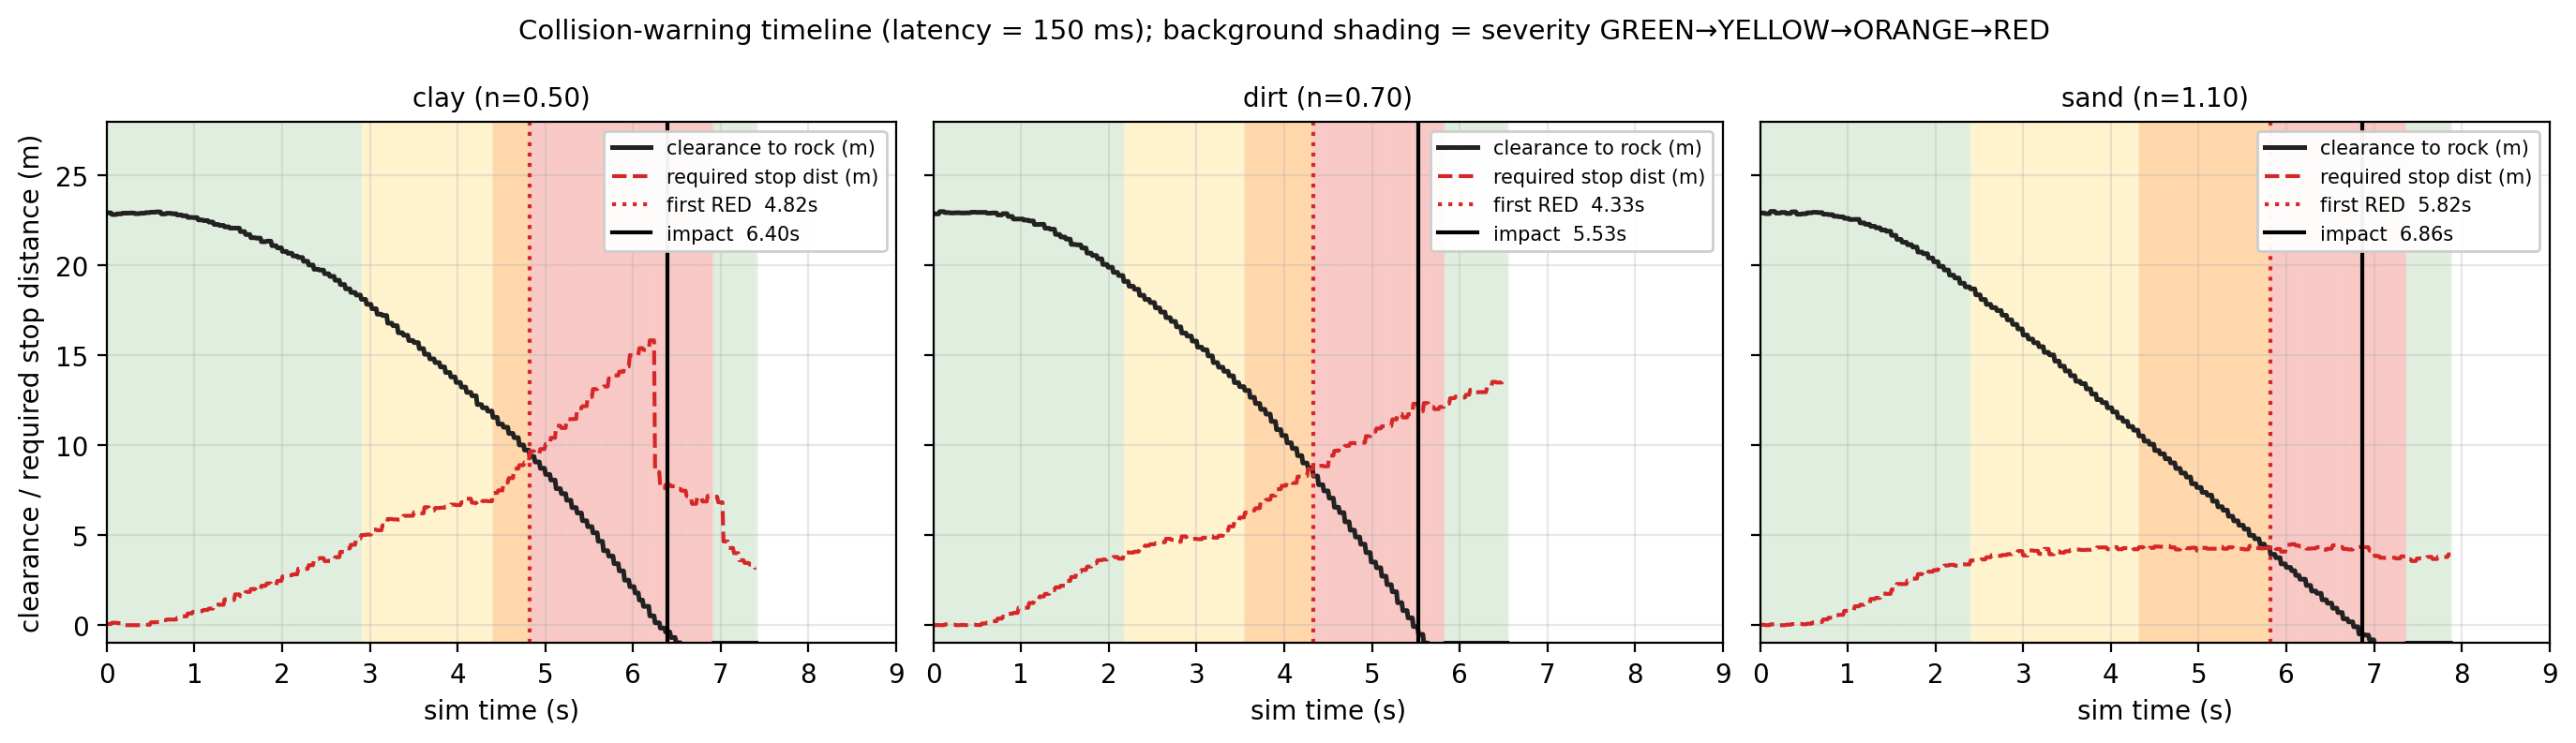
\includegraphics[width=\textwidth]{cw_timeline.png}
  \caption{Severity escalation over time for one representative
    blind-drive run per terrain at $150\,\mathrm{ms}$ one-way delay.
    Background shading is the live severity band (GREEN $\to$ YELLOW
    $\to$ ORANGE $\to$ RED); curves are the chassis clearance to the
    rock (solid) and the warning system's running stopping-distance
    estimate (dashed). The first RED fires when the clearance curve
    drops to the stopping-distance curve.}
  \label{fig:cw_timeline}
\end{figure*}

\paragraph{HIL integration.}
The warning module is wired through the sim node so any HIL
teleoperation round can enable it. Per-tick severity is logged
alongside the existing diagnostics, and severity transitions are
reported on the sim-node console and, when the Irrlicht visualiser
is active, surfaced to the operator as a text banner. When the
online terrain estimator is active, the live $\hat n$ is forwarded
to the warning system on every control message so that the
brake-decel estimate adapts to the estimator's current terrain
belief; otherwise the warning falls back to the nominal $n$ of the
configured terrain preset. The warning never modifies commands, so
it composes freely with any safety filter (none, DOB-CBF, MPPI,
NMPC) used in the same round.

\paragraph{Latency awareness.} An EMA tracker of recent one-way
network delays and a sliding-window jitter estimator inflate the
operator reaction time by $\tau_{r}\!+\!\mathrm{RTT}\!+\!k\sigma$,
where $\sigma$ is the standard deviation of one-way delays over the
last second of received commands. Increasing the latency baseline or
the jitter inflates $d_{\mathrm{stop}}$ and fires the warning
earlier.

\begin{figure}[!t]
  \centering
  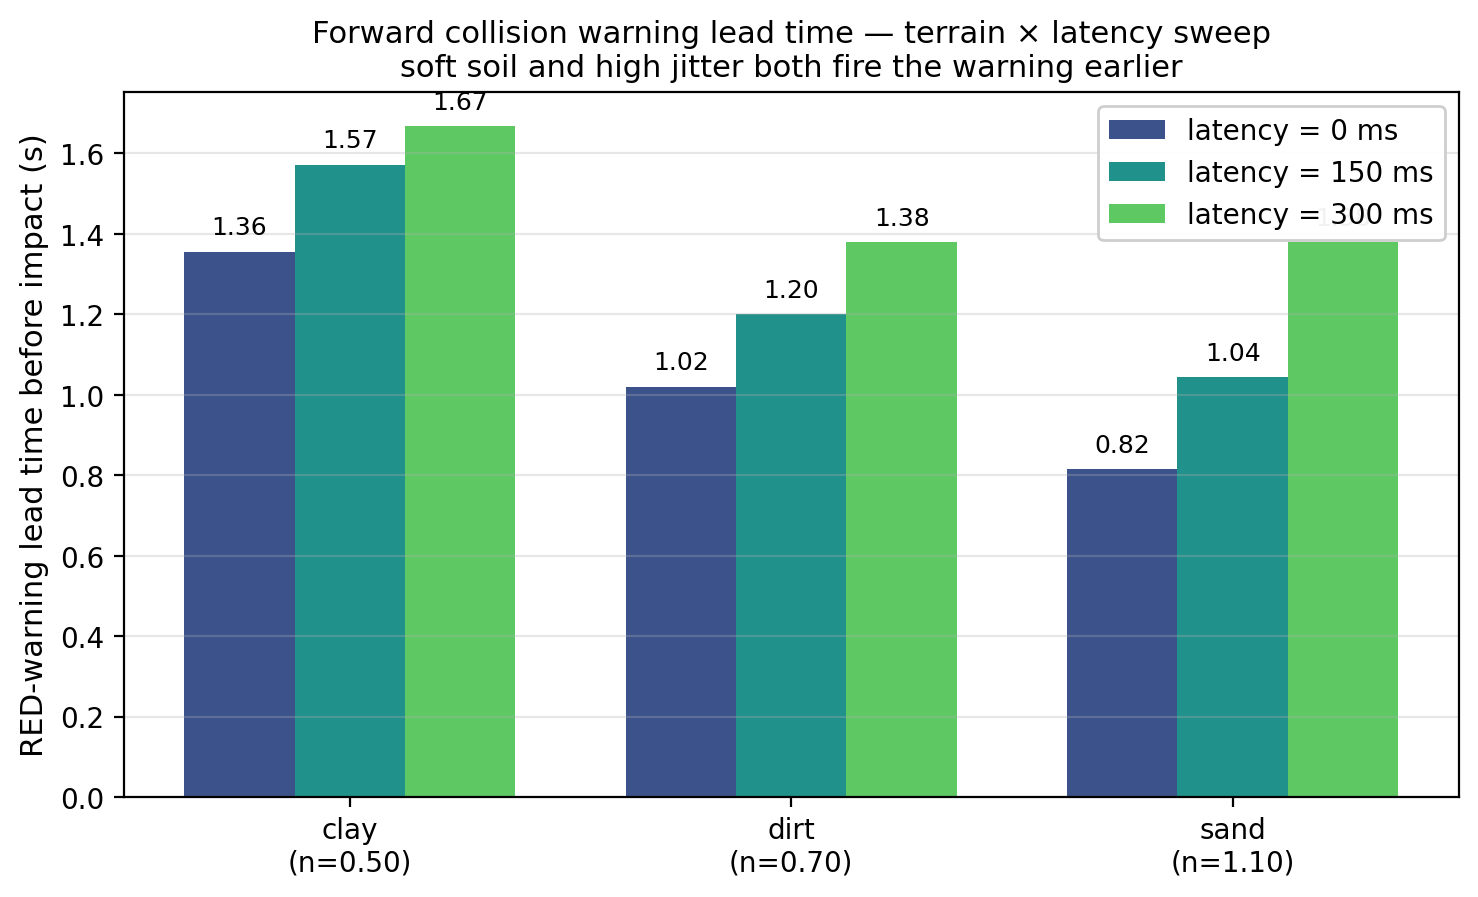
\includegraphics[width=\columnwidth]{cw_lead_vs_terrain.png}
  \caption{Forward collision warning lead time before impact in the
    blind-drive sweep (no MPC, no safety filter, fixed throttle into a
    single rock). Both the terrain-conditioned brake budget and the
    latency-conditioned operator-reaction budget enlarge the required
    stopping distance and therefore advance the first RED warning:
    soft soil (clay) gets the longest lead, and within every terrain
    the lead grows monotonically with the configured one-way delay.}
  \label{fig:cw_lead}
\end{figure}

\begin{table}[!t]
  \renewcommand{\arraystretch}{1.10}
  \caption{Forward collision warning lead time before impact (RED
    severity) under terrain $\times$ latency sweep. The vehicle drives
    blindly at a single $1.2\,\mathrm{m}$ rock with constant throttle.
    Higher latency and softer soil both increase the lead time, as
    designed.}
  \label{tab:cw_lead}
  \centering
  \begin{tabular}{lccc}
    \toprule
     & \textbf{lat=0\,ms} & \textbf{lat=150\,ms} & \textbf{lat=300\,ms}\\
    \midrule
    clay ($\hat n\!=\!0.5$) & $1.56\,\mathrm{s}$ & $1.74\,\mathrm{s}$ & $1.76\,\mathrm{s}$\\
    dirt ($\hat n\!=\!0.7$) & $1.09\,\mathrm{s}$ & $1.25\,\mathrm{s}$ & $1.48\,\mathrm{s}$\\
    sand ($\hat n\!=\!1.1$) & $0.68\,\mathrm{s}$ & $1.00\,\mathrm{s}$ & $1.30\,\mathrm{s}$\\
    \bottomrule
  \end{tabular}
\end{table}

The benchmark
sweeps three terrains and three one-way latency settings.
Table~\ref{tab:cw_lead} reports the time between the first
\textsc{red} warning and the rock impact: on soft clay the warning
fires approximately $1.6\text{--}1.8\,\mathrm{s}$ before impact; on firm
sand the same vehicle reaches the rock with about $0.7\text{--}1.3\,\mathrm{s}$
of lead. The lead time also grows with the configured operator
latency on every terrain (clay $1.56\!\to\!1.76\,\mathrm{s}$ as
latency goes $0\!\to\!300\,\mathrm{ms}$, dirt $1.09\!\to\!1.48$, sand
$0.68\!\to\!1.30$), confirming that the warning correctly couples both
the terrain-conditioned stopping budget and the latency-conditioned
operator-reaction budget.

%======================================================================
\section{Open-Source Benchmarking Suite}
\label{sec:suite}
%======================================================================

A single invocation of the suite's top-level driver executes all of
the autonomous sub-sweeps that produce the non-HIL results reported
in this paper, then merges the resulting figures and CSVs into the
publication set. The paper tier completes
approximately $13{,}000$ Chrono closed-loop trials on a single
24-core workstation; the human-in-the-loop protocol of
Sec.~\ref{sec:safety_hil} is run separately because it requires an
operator at the wheel.

Reproducibility is enforced through a few architectural
choices in the suite itself. Sensor noise is enabled in every trial
so no oracle quantity is observable at inference time. A per-trial
diagnostic CSV is saved alongside each run for post-hoc inspection.
Aggregated KPIs deduplicate on the run key
$(\textit{variant},\,\textit{terrain},\,\textit{path},\,\textit{speed},\,
\textit{bumpiness},\,\textit{seed})$, so a re-run cleanly fills only
the missing cells without overwriting existing rows. The ZeroMQ
publisher retries socket bind with linear backoff to eliminate
TIME\_WAIT races under rapid run cycling, and the publication step
matches result folders by exact timestamp so that closely-named
sweep variants are never conflated.

%======================================================================
\section{Discussion}
\label{sec:disc}
%======================================================================

Two recent threads are directly adjacent to this framework and merit
explicit comparison. Onozuka et al.~\cite{Onozuka25} replace a
terrain-parameter-dependent NN tire model with a physics-informed
structure -- a Janosi saturating shear law wrapped around two small
networks that supply the force coefficients -- and re-fit those
coefficients online by stochastic gradient descent on state-derivative
residuals. The approach is complementary to ours: they fold soil
mechanics into a structured force law where we estimate the soil and
re-condition an unstructured surrogate. A direct adaptation of their
model into the per-axle interface of our acados solver improved
offline force prediction (held-out $R^2_{F_y}$ from $0.35$ to $0.59$)
but underperformed on aggressive transient maneuvers because the
static formulation triggered QP failures in our in-horizon NMPC; a
faithful deployment requires the dedicated curvilinear-coordinate,
wheelspeed-state MPC of~\cite{Onozuka25}, which is out of this paper's
scope. Gupta et al.~\cite{Gupta24} compensate unmodeled dynamics with
a reinforcement-learning residual on top of MPC; in a feasibility
prototype on the same plant the residual closed less than $8\,\%$ of
the residual tracking error and only at the largest model
mismatch -- consistent with our own earlier finding that a learned
dynamics residual offered little benefit on this plant -- so this
paper does not adopt RL compensation.

The empirical evidence supports each architectural choice. The
whole-vehicle neural tire surrogate solves in
${\sim}14\,\mathrm{ms}$ (well within the $100\,\mathrm{ms}$ MPC step)
and reduces median RMS crosstrack error against the
\emph{SCM-calibrated} analytical baselines by $37$--$38\,\%$ in the
live-estimator regime (Table~\ref{tab:tires_estimator}), separating
clearly from them in the tail across the full terrain matrix
(Table~\ref{tab:tires_static}), where even the calibrated baselines
diverge on off-nominal dirt. The asymmetric
throttle disturbance observer increases achieved speed by approximately
$5\,\%$ ($4.06\!\to\!4.26\,\mathrm{m/s}$, $0.61\!\to\!0.64$ of the
g--g profile) at a negligible (${\sim}3\,\mathrm{mm}$) tracking
cost. The two-layer planner-aware stack drives collisions to near zero
($\le 0.20$/run) when paired with either DOB-CBF or MPPI as the
downstream safety filter, the MPPI seed trajectories are essential rather
than auxiliary, the DOB-CBF filter benefits substantially from
re-using the neural surrogate, and both safety filters cut collisions by
${>}90\,\%$ under the learned 5G profile. The forward
collision warning closes the advisory gap the override-style filters
leave open: its analytical stopping-distance prediction lands within
$0.17\,\mathrm{m}$ of the actual Chrono stop ($2.6\times$ better than
the prior hand-tuned fallback), and lead time grows monotonically
with both softer soil and longer one-way delay.

The terrain estimator is intentionally scoped to the sinkage exponent
$n$, which is the parameter that transfers cleanly under closed-loop
sinusoidal excitation. The HIL protocol of
Section~\ref{sec:safety_hil} is implemented with a Logitech G29 and
delayed command/camera channels; the autonomous sweeps provide the
repeatable quantitative evidence, and any session can additionally
enable the forward collision warning alongside the chosen filter.

\subsection{Limitations and scope}
\label{sec:limitations}
This study is conducted entirely in simulation, on a single HMMWV plant
on Chrono's Soil Contact Model. We make no sim-to-real transfer claim:
the contribution is the modular, latency-aware \emph{architecture} and
the relative comparisons it enables on a high-fidelity, widely-used
deformable-terrain plant~\cite{Krenn09,Tasora16}. Those comparisons ---
learned surrogate versus analytical tire model, safety filter versus no safety filter,
estimator-on versus wrong-prior --- are internal to one plant and one
harness, so they are unaffected by any absolute sim-to-real offset; and
the plant is itself a swap point, so porting to hardware or another
terramechanics model is a registration rather than a rewrite. The
neural surrogate is trained and evaluated on the same SCM plant, so the
analytical baselines are calibrated to that plant's mean lateral
friction with a single global parameter set
(Sec.~\ref{sec:tires_static}): the comparison is against a fair,
SCM-calibrated analytical model rather than an uninformative rigid-road baseline, and
the residual gap reflects what a fixed parameterization structurally
cannot capture about terrain-varying deformable forces, not a tuning
deficit.

A characterized floor within the surrogate is the rear-axle lateral
force. Section~\ref{sec:feature_headroom} shows that, unlike the front
axle, rear $F_y$ does not respond to any causal MPC-available feature we
tried --- dynamic vehicle state, kinematic load transfer, per-wheel
sinkage (the multi-pass effect, tested even with ground-truth SCM
sinkage as an oracle), or a $0.32$\,s slip/state history --- all of
which leave it within $4\%$ of the deployed model. We therefore treat
rear $F_y$ as irreducible at the deployed capacity rather than a tuning
target. Separately, the longitudinal channel's soft-soil speed bias is a
dynamics-level motion-resistance term, not a learnable tire feature
($F_x$ RMSE moves at most $3\%$ under the same feature sweep); we compensate it
with the throttle disturbance observer (Sec.~\ref{sec:throttledob})
online, and a feedforward sinkage-drag term in the prediction model is
the natural future replacement.

The online estimator recovers only the sinkage exponent $n$ and
reconstructs the remaining five Bekker--Mohr parameters from $\hat n$
along the clay--dirt--sand preset manifold --- the parameter-known
setting also used by the reference terramechanics estimators
(Sec.~\ref{sec:ukf}). This assumes deployment soils lie near that
manifold; soils with large independent excursions in cohesion, friction,
or stiffness fall outside the present scope, and $n$-recovery degrades
off the manifold. Estimating the full soil vector online, hardware
transfer, and the human-subject teleoperation study the HIL protocol is
built for are the principal directions for future work.

%======================================================================
\section{Conclusion}
\label{sec:conclusion}
%======================================================================
We presented a modular, latency-aware framework that integrates
terrain-adaptive control, online soil estimation, two-layer obstacle
avoidance, and a terrain- and latency-aware collision warning around a
single deformable-terrain plant. The novelty is the \emph{integration}:
where prior work treats terrain adaptation and delay-compensated safety
in isolation, here a differentiable SCM tire surrogate, an online
$n$-estimator that re-conditions it, swappable safety filters, and an
advisory warning share one plant, one messaging substrate, and one
benchmarking harness, so every architectural choice is measured on the
same matrix. Empirically, the surrogate-plus-estimator recovers
near-oracle tracking with no prior terrain knowledge --- within
$\approx\!3\,\mathrm{mm}$ median RMS crosstrack error of the
matched-prior oracle and well below SCM-calibrated analytical baselines;
the deployed proprioceptive-fused UKF tracks $n$ across the deployable
range at $4.5\,\%$ median error; both safety filters cut collisions by
more than $90\,\%$ under a learned 5G latency profile; and the collision
warning predicts stopping distance to $0.17\,\mathrm{m}$. The modular
swap points make each of these a replaceable component rather than a
fixed pipeline, which is what positions the framework for the
hardware-in-the-loop and full-soil-estimation extensions above.

%======================================================================
\section*{Reproducibility}

The complete autonomous sweep, including the non-HIL figures and
CSV-backed tables in this paper, is reproduced by the following single
command in the provided conda environment:
\begin{quote}\small\tt
python benchmarking/run.py --tier paper
\end{quote}
The exact result folders backing each figure are catalogued alongside
the published figures. The HIL rounds are intentionally excluded from
this automated command because they require a human operator; they
are run through a separate human-in-the-loop script.

%======================================================================
\section*{Acknowledgements}

This work builds on the Chrono::HIL framework~\cite{Zhou23} and
Project Chrono~\cite{Tasora16,Serban19}. The 5G traffic profile is
generated using the public N-HiTS-5G implementation released with
Choi et al.~\cite{Choi23}.

\begin{thebibliography}{9}

\bibitem{Bekker69}
  M.~G.~Bekker, \emph{Introduction to Terrain-Vehicle Systems}.
  Ann Arbor, MI: University of Michigan Press, 1969.

\bibitem{Choi23}
  Y.-H.~Choi \emph{et al.}, ``ML-based 5G traffic generation for
  practical simulations using open datasets,''
  \emph{IEEE Commun.\ Mag.}, vol.~61, pp.~130--136, 2023.

\bibitem{Dallas21}
  J.~Dallas \emph{et al.}, ``Terrain adaptive trajectory planning
  and tracking on deformable terrains,''
  \emph{IEEE Trans.\ Veh.\ Technol.},
  vol.~70, no.~11, pp.~11255--11268, 2021.

\bibitem{Krenn09}
  R.~Krenn and G.~Hirzinger, ``SCM -- a soil contact model for
  multi-body system simulations,'' in
  \emph{Proc.\ Int.\ Soc.\ for Terrain-Vehicle Systems (ISTVS)},
  Bremen, Germany, 2009.

\bibitem{Serban19}
  R.~Serban, M.~Taylor, D.~Negrut, and A.~Tasora,
  ``Chrono::Vehicle: template-based ground vehicle modelling and
  simulation,''
  \emph{Int.\ J.\ Veh.\ Perf.}, vol.~5, no.~1, pp.~18--39, 2019.

\bibitem{Shibly05}
  H.~Shibly, K.~Iagnemma, and S.~Dubowsky, ``An equivalent soil
  mechanics formulation for rigid wheels in deformable terrain,''
  \emph{J.\ Terramech.}, vol.~42, no.~1, pp.~1--13, 2005.

\bibitem{Tasora16}
  A.~Tasora \emph{et al.}, ``Chrono: an open source multi-physics
  dynamics engine,'' in
  \emph{High Performance Computing in Science and Engineering},
  pp.~19--49, Springer, 2016.

\bibitem{Zhang25}
  H.~Zhang \emph{et al.}, ``Shared control of teleoperated vehicles
  with delay-compensated safety filtering,'' in
  \emph{Proc.\ IEEE Conf.\ Control Technol.\ Appl.\ (CCTA)},
  pp.~192--199, 2025.

\bibitem{Onozuka25}
  Y.~Onozuka, J.~Dallas, M.~Suminaka, and J.~Subosits,
  ``Adaptive Model Predictive Control on Unknown Deformable Terrains
  Using Physics-Informed Learning Tire Models,'' in
  \emph{Proc.\ IEEE Intelligent Vehicles Symp.\ (IV)}, 2025, pp.~1640--1647.

\bibitem{Gupta24}
  P.~Gupta, J.~M.~Smereka, and Y.~Jia,
  ``Reinforcement learning compensated model predictive control for
  off-road driving on unknown deformable terrain,''
  \emph{arXiv:2408.09253}, 2024.

\bibitem{Zhou23}
  Z.~Zhou \emph{et al.}, ``A Chrono-based framework for large-scale
  traffic simulation with human-in-the-loop,'' 2023.

\end{thebibliography}

\end{document}
